\documentclass[a4paper,12pt]{report}
\usepackage[serie,niveau={1MA1},nfiche={}, annee={Emilie-Gourd, 2024--2025}, auteur={ns},theme={Série MathALÉA}]{packages/bandeaux}
\usepackage{packages/boites}
\usepackage{packages/fontes}
\usepackage{packages/courslatex}
\usepackage{./packages/packages_mathalea}

\newboolean{solution} % Boolean to indicate if solutions should be shown
\newboolean{uuid} % Boolean to indicate if UUID should be shown
\newboolean{link} % Boolean to indicate if a link should be shown
\newcounter{num} % Counter to keep track of exercise numbers

% liens vers des ressources extérieures :
\newcommand{\pathcorrige}{https://raw.githubusercontent.com/smaxx73/Exercices/main/pdf/pdf/} % Path to corrected exercises
\newcommand{\pathnotebook}{https://github.com/smaxx73/Exercices/blob/main/notebook/} % Path to notebooks
\newcommand{\pathexercice}{https://raw.githubusercontent.com/smaxx73/Exercices/main/pdf/pdf_sansol/} % Path to exercises without solutions

% Define the title of the exercise
\newcommand{\titre}[1]{%
	\def\TitreExo{#1} % Set the title for later use
}

% Define the content of the exercise
\newcommand{\contenu}[1]{%
	\def\Contenu{#1} % Set the content for later use
}

% Define the number of points for the exercise
\newcommand{\pts}[1]{%
	\def\Points{#1} % Set the number of points for later use
}

% Define the number of points for the exercise
\newcommand{\piments}[1]{%
	\def\Piments{#1} % Set the number of points for later use
}

% Define the year of the exercise
\newcommand{\annee}[1]{
	\def\Annee{#1} % Set the year for later use
}

% Define the year of the exercise
\newcommand{\organisation}[1]{
	\def\Organisation{#1} % Set the year for later use
}

% Define the correction (solution) of the exercise
\newcommand{\correction}[1]{%
	\def\Solution{#1} % Set the solution for later use
}

% Directly use code as it is
\newcommand{\code}[1]{#1} % Simple passthrough command for code

% Directly use text as it is
\newcommand{\texte}[1]{#1} % Simple passthrough command for text

% Define the correction (solution) of the exercise
\newcommand{\theme}[1]{%
	\def\Theme{#1} % Set the solution for later use
}
% Define the author (currently unused)
\newcommand{\auteur}[1]{} % Placeholder for author

% Command for question text
\newcommand{\question}[1]{#1} % Simple passthrough command for question

% Command for providing a response, shown only if the solution boolean is true
\newcommand{\reponse}[1]{%
	\ifthenelse{\boolean{solution}} % Check if 'solution' is true
	{%
		\begin{solutionbox} % Begin solution box environment
			\begin{footnotesize} #1 \end{footnotesize} % Display the response in small font size
		\end{solutionbox}}{} % End solution box if 'solution' is true
} 

% Move to the next exercise by incrementing the counter
\newcommand{\nextexo}{%
	\addtocounter{num}{1} % Increment exercise counter
	\vspace{1em} % Add vertical space
}


\newcommand{\insertexo}[4]{% contenu, uuid, type (exo/cor/both), upside-down solution
    \input{\path src/#1} % Input the exercise content from the provided path
    \setboolean{uuid}{#2} % Set the uuid boolean
    
    % Start grouping to tightly control scope
    \begingroup
    % Print the exercise if #3 equals "exo" or "both"
    \ifthenelse{\equal{#3}{exo} \OR \equal{#3}{both}}{%
        \noindent % Ensure no extra indentation
        \begin{exo}[\Piments] % Begin question environment with the number of points
            \ifthenelse{\boolean{uuid}}{#1}{} % Include uuid if true
            \Contenu % Insert the content of the exercise
        \end{exo}
    }{} % Otherwise, do nothing
    
    % Print the correction if #3 equals "cor" or "both"
    \ifthenelse{\equal{#3}{cor} \OR \equal{#3}{both}}{%
        \noindent % Ensure no extra indentation
        \ifthenelse{\equal{#4}{true}}{%
            \begin{core-upside} % Use core-upside for upside-down solution
                {\footnotesize \Solution} % Insert the solution
            \end{core-upside}
        }{%
            \begin{core} % Use normal core for regular solution
                \Solution % Insert the solution
            \end{core}
        }%
    }{} % Otherwise, do nothing
    
    \endgroup % End the group
}

% Command to list exercises from a given list
\newcommand{\listexo}[1]{% liste of exercises
	\foreach \ex in #1 { % Iterate over each exercise in the list
		\nextexo % Move to the next exercise
		\insertexo{\ex}{\solution}{\uuid}{\link}{\thenum} % Insert the current exercise with its properties
	}
}

% Counter for QR codes
\newcounter{qrcodenum} % Define a counter to track QR codes

% Command to create a list of QR codes for exercises
\newcommand{\listeqrcode}[2]{% liste d'exercices, initialisation du compteur
\setcounter{qrcodenum}{#2} % Set the initial value for the QR code counter
\noindent
\foreach \exo in #1{ % Iterate over each exercise in the list
	% Create a minipage for each exercise with its number, title, and QR code
	\begin{minipage}{0.24\textwidth}  % Adjust the width to have 4 QR codes per line
		\centering
		\href{\pathcorrige\exo.pdf}{\texttt{Ex \theqrcodenum : \exo \vspace{1em}}}  % Display the number and title of the exercise with a hyperlink
		{\qrcode{\pathcorrige\exo.pdf}}  % Generate the QR code for the exercise
		\par\vspace{2em}  % Add vertical space between QR codes
	\end{minipage}
	% Increment the QR code counter
	\stepcounter{qrcodenum}
}
}



\begin{document}

% @see : https://coopmaths.fr/alea?uuid=8f5d3&id=9ES1-1&n=3&d=10&alea=API3&cd=1&cols=3
\begin{EXO}{}{9ES1-1}
Compléter les programmes de construction qui ont permis d'obtenir ces figures.
\begin{multicols}{3}
\begin{enumerate}[]
	\item \begin{minipage}[t]{\linewidth} Placer 3 points $K$, $L$ et $M$ non alignés puis tracer... 

\medskip
\begin{tikzpicture}[baseline]

    \tikzset{
      point/.style={
        thick,
        draw,
        cross out,
        inner sep=0pt,
        minimum width=5pt,
        minimum height=5pt,
      },
    }
    \clip (-1,-1) rectangle (5,4.5);
    	\draw[color={black}] (-33.63363686569483,-36.99700055226432)--(35.63363686569483,39.19700055226432);
	\draw[color ={black}] (4.2,-0.6)--(-4.178215108038729,10.063182864776564);
	\draw[color ={black}] (0,0)--(4.2,-0.6);
	\draw [color={black}] (-0.5,0.5) node[anchor = center,scale=1, rotate = 0] {K};
	\draw [color={black}] (2,2.7) node[anchor = center,scale=1, rotate = 0] {L};
	\draw [color={black}] (4.7,-0.1) node[anchor = center,scale=1, rotate = 0] {M};
	\draw[color ={{black}},line width = 0.625,opacity = 0.8] (-0.1875,0.1875)--(0.1875,-0.1875);\draw[color ={{black}},line width = 0.625,opacity = 0.8] (-0.1875,-0.1875)--(0.1875,0.1875);\draw[color ={{black}},line width = 0.625,opacity = 0.8] (1.8125,2.3875)--(2.1875,2.0125);\draw[color ={{black}},line width = 0.625,opacity = 0.8] (1.8125,2.0125)--(2.1875,2.3875);\draw[color ={{black}},line width = 0.625,opacity = 0.8] (4.0125,-0.4125)--(4.3875,-0.7875);\draw[color ={{black}},line width = 0.625,opacity = 0.8] (4.0125,-0.7875)--(4.3875,-0.4125);

\end{tikzpicture}\\ \end{minipage}
	\item \begin{minipage}[t]{\linewidth} Placer 3 points $F$, $G$ et $H$ non alignés puis tracer... 

\medskip
\begin{tikzpicture}[baseline]

    \tikzset{
      point/.style={
        thick,
        draw,
        cross out,
        inner sep=0pt,
        minimum width=5pt,
        minimum height=5pt,
      },
    }
    \clip (-1,-1) rectangle (5,4.5);
    	\draw[color={black}] (-33.63363686569483,-36.99700055226432)--(35.63363686569483,39.19700055226432);
	\draw[color ={black}] (2,2.2)--(4.2,-0.6);
	\draw[color ={black}] (0,0)--(14.09949420655672,-2.014213458079531);
	\draw [color={black}] (-0.5,0.5) node[anchor = center,scale=1, rotate = 0] {F};
	\draw [color={black}] (2,2.7) node[anchor = center,scale=1, rotate = 0] {G};
	\draw [color={black}] (4.7,-0.1) node[anchor = center,scale=1, rotate = 0] {H};
	\draw[color ={{black}},line width = 0.625,opacity = 0.8] (-0.1875,0.1875)--(0.1875,-0.1875);\draw[color ={{black}},line width = 0.625,opacity = 0.8] (-0.1875,-0.1875)--(0.1875,0.1875);\draw[color ={{black}},line width = 0.625,opacity = 0.8] (1.8125,2.3875)--(2.1875,2.0125);\draw[color ={{black}},line width = 0.625,opacity = 0.8] (1.8125,2.0125)--(2.1875,2.3875);\draw[color ={{black}},line width = 0.625,opacity = 0.8] (4.0125,-0.4125)--(4.3875,-0.7875);\draw[color ={{black}},line width = 0.625,opacity = 0.8] (4.0125,-0.7875)--(4.3875,-0.4125);

\end{tikzpicture}\\ \end{minipage}
	\item \begin{minipage}[t]{\linewidth} Placer 3 points $T$, $U$ et $V$ non alignés puis tracer... 

\medskip
\begin{tikzpicture}[baseline]

    \tikzset{
      point/.style={
        thick,
        draw,
        cross out,
        inner sep=0pt,
        minimum width=5pt,
        minimum height=5pt,
      },
    }
    \clip (-1,-1) rectangle (5,4.5);
    	\draw[color ={black}] (0,0)--(8.726727373138967,9.599400110452864);
	\draw[color={black}] (-28.891075540193643,41.515914323882825)--(35.09107554019364,-39.915914323882824);
	\draw[color={black}] (-49.497471032783594,7.071067290397656)--(53.6974710327836,-7.671067290397656);
	\draw [color={black}] (-0.5,0.5) node[anchor = center,scale=1, rotate = 0] {T};
	\draw [color={black}] (2,2.7) node[anchor = center,scale=1, rotate = 0] {U};
	\draw [color={black}] (4.7,-0.1) node[anchor = center,scale=1, rotate = 0] {V};
	\draw[color ={{black}},line width = 0.625,opacity = 0.8] (-0.1875,0.1875)--(0.1875,-0.1875);\draw[color ={{black}},line width = 0.625,opacity = 0.8] (-0.1875,-0.1875)--(0.1875,0.1875);\draw[color ={{black}},line width = 0.625,opacity = 0.8] (1.8125,2.3875)--(2.1875,2.0125);\draw[color ={{black}},line width = 0.625,opacity = 0.8] (1.8125,2.0125)--(2.1875,2.3875);\draw[color ={{black}},line width = 0.625,opacity = 0.8] (4.0125,-0.4125)--(4.3875,-0.7875);\draw[color ={{black}},line width = 0.625,opacity = 0.8] (4.0125,-0.7875)--(4.3875,-0.4125);

\end{tikzpicture}\\ \end{minipage}
\end{enumerate}
\end{multicols}
\end{EXO}

% @see : https://coopmaths.fr/alea?uuid=8f5d3&id=9ES1-1&n=3&d=10&alea=VbwM&cd=1&cols=3
\begin{EXO}{}{9ES1-1}
Compléter les programmes de construction qui ont permis d'obtenir ces figures.
\begin{multicols}{3}
\begin{enumerate}[]
	\item \begin{minipage}[t]{\linewidth} Placer 3 points $H$, $I$ et $J$ non alignés puis tracer... 

\medskip
\begin{tikzpicture}[baseline]

    \tikzset{
      point/.style={
        thick,
        draw,
        cross out,
        inner sep=0pt,
        minimum width=5pt,
        minimum height=5pt,
      },
    }
    \clip (-1,-1) rectangle (5,4.5);
    	\draw[color ={black}] (0,0)--(8.726727373138967,9.599400110452864);
	\draw[color ={black}] (2,2.2)--(4.2,-0.6);
	\draw[color ={black}] (4.2,-0.6)--(-9.899494206556719,1.4142134580795311);
	\draw [color={black}] (-0.5,0.5) node[anchor = center,scale=1, rotate = 0] {H};
	\draw [color={black}] (2,2.7) node[anchor = center,scale=1, rotate = 0] {I};
	\draw [color={black}] (4.7,-0.1) node[anchor = center,scale=1, rotate = 0] {J};
	\draw[color ={{black}},line width = 0.625,opacity = 0.8] (-0.1875,0.1875)--(0.1875,-0.1875);\draw[color ={{black}},line width = 0.625,opacity = 0.8] (-0.1875,-0.1875)--(0.1875,0.1875);\draw[color ={{black}},line width = 0.625,opacity = 0.8] (1.8125,2.3875)--(2.1875,2.0125);\draw[color ={{black}},line width = 0.625,opacity = 0.8] (1.8125,2.0125)--(2.1875,2.3875);\draw[color ={{black}},line width = 0.625,opacity = 0.8] (4.0125,-0.4125)--(4.3875,-0.7875);\draw[color ={{black}},line width = 0.625,opacity = 0.8] (4.0125,-0.7875)--(4.3875,-0.4125);

\end{tikzpicture}\\ \end{minipage}
	\item \begin{minipage}[t]{\linewidth} Placer 3 points $V$, $W$ et $X$ non alignés puis tracer... 

\medskip
\begin{tikzpicture}[baseline]

    \tikzset{
      point/.style={
        thick,
        draw,
        cross out,
        inner sep=0pt,
        minimum width=5pt,
        minimum height=5pt,
      },
    }
    \clip (-1,-1) rectangle (5,4.5);
    	\draw[color={black}] (-33.63363686569483,-36.99700055226432)--(35.63363686569483,39.19700055226432);
	\draw[color ={black}] (2,2.2)--(4.2,-0.6);
	\draw[color={black}] (-49.497471032783594,7.071067290397656)--(53.6974710327836,-7.671067290397656);
	\draw [color={black}] (-0.5,0.5) node[anchor = center,scale=1, rotate = 0] {V};
	\draw [color={black}] (2,2.7) node[anchor = center,scale=1, rotate = 0] {W};
	\draw [color={black}] (4.7,-0.1) node[anchor = center,scale=1, rotate = 0] {X};
	\draw[color ={{black}},line width = 0.625,opacity = 0.8] (-0.1875,0.1875)--(0.1875,-0.1875);\draw[color ={{black}},line width = 0.625,opacity = 0.8] (-0.1875,-0.1875)--(0.1875,0.1875);\draw[color ={{black}},line width = 0.625,opacity = 0.8] (1.8125,2.3875)--(2.1875,2.0125);\draw[color ={{black}},line width = 0.625,opacity = 0.8] (1.8125,2.0125)--(2.1875,2.3875);\draw[color ={{black}},line width = 0.625,opacity = 0.8] (4.0125,-0.4125)--(4.3875,-0.7875);\draw[color ={{black}},line width = 0.625,opacity = 0.8] (4.0125,-0.7875)--(4.3875,-0.4125);

\end{tikzpicture}\\ \end{minipage}
	\item \begin{minipage}[t]{\linewidth} Placer 3 points $A$, $B$ et $C$ non alignés puis tracer... 

\medskip
\begin{tikzpicture}[baseline]

    \tikzset{
      point/.style={
        thick,
        draw,
        cross out,
        inner sep=0pt,
        minimum width=5pt,
        minimum height=5pt,
      },
    }
    \clip (-1,-1) rectangle (5,4.5);
    	\draw[color ={black}] (0,0)--(2,2.2);
	\draw[color={black}] (-28.891075540193643,41.515914323882825)--(35.09107554019364,-39.915914323882824);
	\draw[color ={black}] (4.2,-0.6)--(-9.899494206556719,1.4142134580795311);
	\draw [color={black}] (-0.5,0.5) node[anchor = center,scale=1, rotate = 0] {A};
	\draw [color={black}] (2,2.7) node[anchor = center,scale=1, rotate = 0] {B};
	\draw [color={black}] (4.7,-0.1) node[anchor = center,scale=1, rotate = 0] {C};
	\draw[color ={{black}},line width = 0.625,opacity = 0.8] (-0.1875,0.1875)--(0.1875,-0.1875);\draw[color ={{black}},line width = 0.625,opacity = 0.8] (-0.1875,-0.1875)--(0.1875,0.1875);\draw[color ={{black}},line width = 0.625,opacity = 0.8] (1.8125,2.3875)--(2.1875,2.0125);\draw[color ={{black}},line width = 0.625,opacity = 0.8] (1.8125,2.0125)--(2.1875,2.3875);\draw[color ={{black}},line width = 0.625,opacity = 0.8] (4.0125,-0.4125)--(4.3875,-0.7875);\draw[color ={{black}},line width = 0.625,opacity = 0.8] (4.0125,-0.7875)--(4.3875,-0.4125);

\end{tikzpicture}\\ \end{minipage}
\end{enumerate}
\end{multicols}
\end{EXO}

% @see : https://coopmaths.fr/alea?uuid=e8f0b&id=9ES1-3&n=1&d=10&s=1&alea=YLub&cd=1&cols=1
\begin{EXO}{}{9ES1-3}


 À l'aide du schéma ci-dessous, déterminer :\\- deux segments de même longueur ;\\- le milieu d'un segment ;\\- un triangle rectangle ;\\- un triangle isocèle.\\\begin{tikzpicture}[baseline]

    \tikzset{
      point/.style={
        thick,
        draw,
        cross out,
        inner sep=0pt,
        minimum width=5pt,
        minimum height=5pt,
      },
    }
    \clip (-2.3673862487200577,-5.821772945971886) rectangle (7.394818203498206,2.574511522493027);
    	\draw[color ={black},decorate,decoration={random steps , amplitude = 1pt}] (0,0)--(-1.3673862487200579,-3.97117801751713);
	\draw[color ={black},decorate,decoration={random steps , amplitude = 1pt}] (0,0)--(6.394818203498206,-2.847156501530601);
	\draw[color ={black},decorate,decoration={random steps , amplitude = 1pt}] (-1.3673862487200579,-3.97117801751713)--(6.394818203498206,-2.847156501530601);
	\draw[color ={black},decorate,decoration={random steps , amplitude = 1pt}] (2.9067355470446388,-1.2941620461502732)--(4.109630327279606,1.074511522493027);
	\draw[color ={black},decorate,decoration={random steps , amplitude = 1pt}] (6.394818203498206,-2.847156501530601)--(4.109630327279606,1.074511522493027);
	\draw[color ={black},decorate,decoration={random steps , amplitude = 1pt}] (0,0)--(4.109630327279606,1.074511522493027);
	\draw[color ={black},decorate,decoration={random steps , amplitude = 1pt}] (6.394818203498206,-2.847156501530601)--(2.918271164636011,-4.821772945971886);
	\draw[color ={black},decorate,decoration={random steps , amplitude = 1pt}] (-1.3673862487200579,-3.97117801751713)--(2.918271164636011,-4.821772945971886);
	\draw[color={black},decorate,decoration={random steps , segment length=3pt, amplitude = 1pt}] (-0.13,-0.38)--(0.25,-0.51)--(0.37,-0.16);
	\draw [color={black}] (2.05,0.54) node[anchor = center,scale=2, rotate = 14] {//};
\draw [color={black}] (5.25,-0.89) node[anchor = center,scale=2, rotate = -59] {//};

	\draw [color={black}] (1.45,-0.65) node[anchor = center,scale=2, rotate = -24] {|||};
\draw [color={black}] (4.65,-2.07) node[anchor = center,scale=2, rotate = -24] {|||};

	\draw [color={black}] (0.78,-4.4) node[anchor = center,scale=2, rotate = -11] {O};
\draw [color={black}] (4.66,-3.83) node[anchor = center,scale=2, rotate = 29] {O};

	\draw [color={black}] (-0.5,0) node[anchor = center,scale=1, rotate = 0] {V};
	\draw [color={black}] (-1.37,-4.47) node[anchor = center,scale=1, rotate = 0] {W};
	\draw [color={black}] (6.89,-2.85) node[anchor = center,scale=1, rotate = 0] {X};
	\draw [color={black}] (2.92,-5.32) node[anchor = center,scale=1, rotate = 0] {Y};
	\draw [color={black}] (2.91,-1.79) node[anchor = center,scale=1, rotate = 0] {T};
	\draw [color={black}] (4.11,1.57) node[anchor = center,scale=1, rotate = 0] {U};
	\draw[color={black},decorate,decoration={random steps , segment length=3pt, amplitude = 1pt}] (2.54,-1.13)--(2.7,-0.77)--(3.09,-0.94);

\end{tikzpicture}\\
\end{EXO}

% @see : https://coopmaths.fr/alea?uuid=02320&id=9ES1-4&n=2&d=10&alea=R0fA&cd=1&cols=1
\begin{EXO}{}{9ES1-4}


\begin{enumerate}[]
	\item Graphiquement, les points suivants sont-ils alignés ?\\\begin{tikzpicture}[baseline]

    \tikzset{
      point/.style={
        thick,
        draw,
        cross out,
        inner sep=0pt,
        minimum width=5pt,
        minimum height=5pt,
      },
    }
    \clip (-2,-2) rectangle (7.6,2.56);
    	\draw[color ={{black}},line width = 0.625,opacity = 0.8] (-0.0625,0.0625)--(0.0625,-0.0625);\draw[color ={{black}},line width = 0.625,opacity = 0.8] (-0.0625,-0.0625)--(0.0625,0.0625);
	\draw[color ={{black}},line width = 0.625,opacity = 0.8] (2.7375,0.34249999999999997)--(2.8625,0.21749999999999997);\draw[color ={{black}},line width = 0.625,opacity = 0.8] (2.7375,0.21749999999999997)--(2.8625,0.34249999999999997);
	\draw [color={black}] (0,-0.5) node[anchor = center,scale=1, rotate = 0] {B};
	\draw [color={black}] (2.8,-0.22) node[anchor = center,scale=1, rotate = 0] {W};
	\draw[color ={{black}},line width = 0.625,opacity = 0.8] (5.5375,0.6224999999999999)--(5.6625,0.49749999999999994);\draw[color ={{black}},line width = 0.625,opacity = 0.8] (5.5375,0.49749999999999994)--(5.6625,0.6224999999999999);
	\draw [color={black}] (5.6,0.06) node[anchor = center,scale=1, rotate = 0] {Y};

\end{tikzpicture}\\
	\item Graphiquement, les points suivants sont-ils alignés ?\\\begin{tikzpicture}[baseline]

    \tikzset{
      point/.style={
        thick,
        draw,
        cross out,
        inner sep=0pt,
        minimum width=5pt,
        minimum height=5pt,
      },
    }
    \clip (-2,-3.16) rectangle (7.8,2);
    	\draw[color ={{black}},line width = 0.625,opacity = 0.8] (-0.0625,0.0625)--(0.0625,-0.0625);\draw[color ={{black}},line width = 0.625,opacity = 0.8] (-0.0625,-0.0625)--(0.0625,0.0625);
	\draw[color ={{black}},line width = 0.625,opacity = 0.8] (2.1375,-0.37750000000000006)--(2.2625,-0.5025000000000001);\draw[color ={{black}},line width = 0.625,opacity = 0.8] (2.1375,-0.5025000000000001)--(2.2625,-0.37750000000000006);
	\draw [color={black}] (0,0.5) node[anchor = center,scale=1, rotate = 0] {I};
	\draw [color={black}] (2.2,0.06) node[anchor = center,scale=1, rotate = 0] {D};
	\draw[color ={{black}},line width = 0.625,opacity = 0.8] (5.7375,-0.5974999999999999)--(5.8625,-0.7224999999999999);\draw[color ={{black}},line width = 0.625,opacity = 0.8] (5.7375,-0.7224999999999999)--(5.8625,-0.5974999999999999);
	\draw [color={black}] (5.8,-0.16) node[anchor = center,scale=1, rotate = 0] {X};

\end{tikzpicture}\\
\end{enumerate}
\end{EXO}

% @see : https://coopmaths.fr/alea?uuid=a8f1f&id=9ES1-6&n=8&d=10&alea=4Bhs&cd=1&cols=4
\begin{EXO}{}{9ES1-6}
Compléter en utilisant les symboles $\in$ et $\notin$.

\begin{tikzpicture}[baseline]

    \tikzset{
      point/.style={
        thick,
        draw,
        cross out,
        inner sep=0pt,
        minimum width=5pt,
        minimum height=5pt,
      },
    }
    \clip (-4.9544232590366235,-2.520944533000791) rectangle (2,4.298133329356935);
    	
	\draw [color={black}] (-2.48,1.65) node[anchor = center,scale=1, rotate = 0] {O};
	\draw [color={black}] (-0.36,-0.28) node[anchor = center,scale=1, rotate = 0] {B};
	\draw [color={black}] (-3.35,-0.82) node[anchor = center,scale=1, rotate = 0] {U};
	
	\draw [color={black}] (0.37,-0.34) node[anchor = center,scale=1, rotate = 0] {F};
	\draw [color={black}] (-2.21,2.71) node[anchor = center,scale=1, rotate = 0] {R};
	\draw [color={black}] (-1.34,0.12) node[anchor = center,scale=1, rotate = 0] {C};
	\draw[color ={black}] (0,0)--(-1.9283628290596182,2.298133329356934);
	\draw[color ={black}] (-1.9283628290596182,2.298133329356934)--(-2.3387870010504206,1.1705021844138437);
	\draw[color ={black}] (0,0)--(-2.3387870010504206,1.1705021844138437);
	\draw[color ={black}] (-1.9283628290596182,2.298133329356934)--(2.8816859424550527,-8.557439868129924);
	\draw[color ={black}] (0,0)--(-10.692196819929421,-1.8853227823988066);
	\draw[color ={black}] (-1.9283628290596182,2.298133329356934)--(-5.758988434307108,-8.226424023445245);

\end{tikzpicture}\\\begin{multicols}{4}
\begin{enumerate}[]
	\item \begin{minipage}[t]{\linewidth} $C$ $\ldots{}$ [$CO$] \end{minipage}
	\item \begin{minipage}[t]{\linewidth} $O$ $\ldots{}$ [$UR$] \end{minipage}
	\item \begin{minipage}[t]{\linewidth} $B$ $\ldots{}$ ($RC$) \end{minipage}
	\item \begin{minipage}[t]{\linewidth} $F$ $\ldots{}$ [$BU$) \end{minipage}
	\item \begin{minipage}[t]{\linewidth} $O$ $\ldots{}$ ($BC$) \end{minipage}
	\item \begin{minipage}[t]{\linewidth} $C$ $\ldots{}$ [$BU$) \end{minipage}
	\item \begin{minipage}[t]{\linewidth} $C$ $\ldots{}$ [$RB$] \end{minipage}
	\item \begin{minipage}[t]{\linewidth} $U$ $\ldots{}$ ($FO$) \end{minipage}
\end{enumerate}
\end{multicols}
\end{EXO}

% @see : https://coopmaths.fr/alea?uuid=83763&id=9ES1-8&n=3&d=10&alea=5QGe&cd=1&cols=1
\begin{EXO}{}{9ES1-8}
Entourer la bonne figure.

\begin{enumerate}[]
	\item La demi-droite d'origine $N$ passant par $O$.\\\begin{tikzpicture}[baseline,scale = 0.4]

    \tikzset{
      point/.style={
        thick,
        draw,
        cross out,
        inner sep=0pt,
        minimum width=5pt,
        minimum height=5pt,
      },
    }
    \clip (-2,-2) rectangle (6,6);
    	\draw [color={black}] (0,0.5) node[anchor = center,scale=1, rotate = 0] {N};
	\draw [color={black}] (4,3.5) node[anchor = center,scale=1, rotate = 0] {O};
	\draw[color ={black},|-|] (0,0)--(4,3);
	\draw[color ={black}] (4,3)--(-8,-6);

\end{tikzpicture}\begin{tikzpicture}[baseline,scale = 0.4]

    \tikzset{
      point/.style={
        thick,
        draw,
        cross out,
        inner sep=0pt,
        minimum width=5pt,
        minimum height=5pt,
      },
    }
    \clip (-2,-2) rectangle (6,6);
    	\draw [color={black}] (0,0.5) node[anchor = center,scale=1, rotate = 0] {N};
	\draw [color={black}] (4,3.5) node[anchor = center,scale=1, rotate = 0] {O};
	\draw[color ={black},|-|] (0,0)--(4,3);
	\draw[color={black}] (-40,-30)--(44,33);

\end{tikzpicture}\begin{tikzpicture}[baseline,scale = 0.4]

    \tikzset{
      point/.style={
        thick,
        draw,
        cross out,
        inner sep=0pt,
        minimum width=5pt,
        minimum height=5pt,
      },
    }
    \clip (-2,-2) rectangle (6,6);
    	\draw [color={black}] (0,0.5) node[anchor = center,scale=1, rotate = 0] {N};
	\draw [color={black}] (4,3.5) node[anchor = center,scale=1, rotate = 0] {O};
	\draw[color ={black},|-|] (0,0)--(4,3);

\end{tikzpicture}\begin{tikzpicture}[baseline,scale = 0.4]

    \tikzset{
      point/.style={
        thick,
        draw,
        cross out,
        inner sep=0pt,
        minimum width=5pt,
        minimum height=5pt,
      },
    }
    \clip (-2,-2) rectangle (6,6);
    	\draw [color={black}] (0,0.5) node[anchor = center,scale=1, rotate = 0] {N};
	\draw [color={black}] (4,3.5) node[anchor = center,scale=1, rotate = 0] {O};
	\draw[color ={black},|-|] (0,0)--(4,3);
	\draw[color ={black}] (0,0)--(12,9);

\end{tikzpicture}
	\item Le segment d'extrémités $Q$ et $R$.\\\begin{tikzpicture}[baseline,scale = 0.4]

    \tikzset{
      point/.style={
        thick,
        draw,
        cross out,
        inner sep=0pt,
        minimum width=5pt,
        minimum height=5pt,
      },
    }
    \clip (-2,-2) rectangle (6,6);
    	\draw [color={black}] (0,0.5) node[anchor = center,scale=1, rotate = 0] {Q};
	\draw [color={black}] (4,1.5) node[anchor = center,scale=1, rotate = 0] {R};
	\draw[color ={black},|-|] (0,0)--(4,1);
	\draw[color={black}] (-48.507120602768886,-12.126780150692221)--(52.507120602768886,13.126780150692221);

\end{tikzpicture}\begin{tikzpicture}[baseline,scale = 0.4]

    \tikzset{
      point/.style={
        thick,
        draw,
        cross out,
        inner sep=0pt,
        minimum width=5pt,
        minimum height=5pt,
      },
    }
    \clip (-2,-2) rectangle (6,6);
    	\draw [color={black}] (0,0.5) node[anchor = center,scale=1, rotate = 0] {Q};
	\draw [color={black}] (4,1.5) node[anchor = center,scale=1, rotate = 0] {R};
	\draw[color ={black},|-|] (0,0)--(4,1);
	\draw[color ={black}] (4,1)--(-9.701424120553776,-2.425356030138444);

\end{tikzpicture}\begin{tikzpicture}[baseline,scale = 0.4]

    \tikzset{
      point/.style={
        thick,
        draw,
        cross out,
        inner sep=0pt,
        minimum width=5pt,
        minimum height=5pt,
      },
    }
    \clip (-2,-2) rectangle (6,6);
    	\draw [color={black}] (0,0.5) node[anchor = center,scale=1, rotate = 0] {Q};
	\draw [color={black}] (4,1.5) node[anchor = center,scale=1, rotate = 0] {R};
	\draw[color ={black},|-|] (0,0)--(4,1);
	\draw[color ={black}] (0,0)--(13.701424120553776,3.425356030138444);

\end{tikzpicture}\begin{tikzpicture}[baseline,scale = 0.4]

    \tikzset{
      point/.style={
        thick,
        draw,
        cross out,
        inner sep=0pt,
        minimum width=5pt,
        minimum height=5pt,
      },
    }
    \clip (-2,-2) rectangle (6,6);
    	\draw [color={black}] (0,0.5) node[anchor = center,scale=1, rotate = 0] {Q};
	\draw [color={black}] (4,1.5) node[anchor = center,scale=1, rotate = 0] {R};
	\draw[color ={black},|-|] (0,0)--(4,1);

\end{tikzpicture}
	\item La demi-droite d'origine $M$ passant par $L$.\\\begin{tikzpicture}[baseline,scale = 0.4]

    \tikzset{
      point/.style={
        thick,
        draw,
        cross out,
        inner sep=0pt,
        minimum width=5pt,
        minimum height=5pt,
      },
    }
    \clip (-2,-2) rectangle (6,6);
    	\draw [color={black}] (0,0.5) node[anchor = center,scale=1, rotate = 0] {L};
	\draw [color={black}] (4,-0.5) node[anchor = center,scale=1, rotate = 0] {M};
	\draw[color ={black},|-|] (0,0)--(4,-1);
	\draw[color ={black}] (4,-1)--(-9.701424120553776,2.425356030138444);

\end{tikzpicture}\begin{tikzpicture}[baseline,scale = 0.4]

    \tikzset{
      point/.style={
        thick,
        draw,
        cross out,
        inner sep=0pt,
        minimum width=5pt,
        minimum height=5pt,
      },
    }
    \clip (-2,-2) rectangle (6,6);
    	\draw [color={black}] (0,0.5) node[anchor = center,scale=1, rotate = 0] {L};
	\draw [color={black}] (4,-0.5) node[anchor = center,scale=1, rotate = 0] {M};
	\draw[color ={black},|-|] (0,0)--(4,-1);

\end{tikzpicture}\begin{tikzpicture}[baseline,scale = 0.4]

    \tikzset{
      point/.style={
        thick,
        draw,
        cross out,
        inner sep=0pt,
        minimum width=5pt,
        minimum height=5pt,
      },
    }
    \clip (-2,-2) rectangle (6,6);
    	\draw [color={black}] (0,0.5) node[anchor = center,scale=1, rotate = 0] {L};
	\draw [color={black}] (4,-0.5) node[anchor = center,scale=1, rotate = 0] {M};
	\draw[color ={black},|-|] (0,0)--(4,-1);
	\draw[color={black}] (-48.507120602768886,12.126780150692221)--(52.507120602768886,-13.126780150692221);

\end{tikzpicture}\begin{tikzpicture}[baseline,scale = 0.4]

    \tikzset{
      point/.style={
        thick,
        draw,
        cross out,
        inner sep=0pt,
        minimum width=5pt,
        minimum height=5pt,
      },
    }
    \clip (-2,-2) rectangle (6,6);
    	\draw [color={black}] (0,0.5) node[anchor = center,scale=1, rotate = 0] {L};
	\draw [color={black}] (4,-0.5) node[anchor = center,scale=1, rotate = 0] {M};
	\draw[color ={black},|-|] (0,0)--(4,-1);
	\draw[color ={black}] (0,0)--(13.701424120553776,-3.425356030138444);

\end{tikzpicture}
\end{enumerate}
\end{EXO}

% @see : https://coopmaths.fr/alea?uuid=03b49&id=9ES1-9&n=1&d=10&s=3&s2=true&s3=6&alea=TfOy&cd=1&cols=1
\begin{EXO}{}{9ES1-9}
Cocher la (ou les) bonne(s) réponse(s).

 \begin{tikzpicture}[baseline]

    \tikzset{
      point/.style={
        thick,
        draw,
        cross out,
        inner sep=0pt,
        minimum width=5pt,
        minimum height=5pt,
      },
    }
    \clip (-4.194061104857512,-4.364032260820166) rectangle (4.988584094275237,4.364032260820166);
    	\draw[color={black},fill opacity = 1.1] (0,0) circle (3);
	\draw [color={black}] (0,0.5) node[anchor = center,scale=1, rotate = 0] {V};
	\draw[color ={{black}},line width = 0.625,opacity = 0.8] (-0.1875,0.1875)--(0.1875,-0.1875);\draw[color ={{black}},line width = 0.625,opacity = 0.8] (-0.1875,-0.1875)--(0.1875,0.1875);
	\draw[color ={black}] (0,0)--(2.1580194010159524,-2.0839751113769927);
	\draw[color ={black}] (-1.846984425976974,-2.3640322608201663)--(1.846984425976974,2.3640322608201663);
	\draw[color ={black}] (2.988584094275237,-0.26146722824297497)--(-2.1940611048575116,2.0459950801874958);
	
	\draw [color={black}] (2.46,-2.48) node[anchor = center,scale=1, rotate = 0] {R};
	\draw [color={black}] (-2.21,-2.71) node[anchor = center,scale=1, rotate = 0] {C};
	\draw [color={black}] (2.08,2.81) node[anchor = center,scale=1, rotate = 0] {N};
	\draw [color={black}] (3.49,-0.3) node[anchor = center,scale=1, rotate = 0] {T};
	\draw [color={black}] (-2.59,2.35) node[anchor = center,scale=1, rotate = 0] {E};
	\draw [color={blue}] (-0.92,-1.18) node[anchor = center,scale=1, rotate = -308] {//};
\draw [color={blue}] (0.92,1.18) node[anchor = center,scale=1, rotate = 52] {//};
\draw [color={blue}] (1.08,-1.04) node[anchor = center,scale=1, rotate = -44] {//};


\end{tikzpicture}\\\\\textbf {a.} Un rayon est ...	$\square\;$ [$TE$]\qquad $\square\;$ $VR$\qquad $\square\;$ $V$\qquad $\square\;$ $CN$\qquad $\square\;$ [$VR$]\qquad $\square\;$ [$CN$]\qquad 

\medskip
\textbf {b.} Une corde est ...	$\square\;$ [$VR$]\qquad $\square\;$ $V$\qquad $\square\;$ [$TE$]\qquad $\square\;$ $CN$\qquad $\square\;$ [$CN$]\qquad $\square\;$ $VR$\qquad 

\medskip
\textbf {c.} [$CN$] est ...	$\square\;$ le centre du cercle, qui est aussi le milieu de [CN]\qquad $\square\;$ un diamètre\qquad $\square\;$ le diamètre\qquad $\square\;$ le rayon\qquad $\square\;$ un rayon\qquad $\square\;$ une corde\qquad 

\medskip
\textbf {d.} $VR$ est ...	$\square\;$ le rayon\qquad $\square\;$ le diamètre\qquad $\square\;$ une corde\qquad $\square\;$ un diamètre\qquad $\square\;$ le centre du cercle, qui est aussi le milieu de [CN]\qquad $\square\;$ un rayon\qquad 

\medskip
\textbf {e.} $V$ est ...	$\square\;$ le rayon\qquad $\square\;$ le diamètre\qquad $\square\;$ un diamètre\qquad $\square\;$ une corde\qquad $\square\;$ un rayon\qquad $\square\;$ le centre du cercle, qui est aussi le milieu de [CN]\qquad 

\medskip
\textbf {f.} Le diamètre est ...	$\square\;$ [$TE$]\qquad $\square\;$ $VR$\qquad $\square\;$ [$CN$]\qquad $\square\;$ [$VR$]\qquad $\square\;$ $V$\qquad $\square\;$ $CN$\qquad 

\medskip

\end{EXO}

% @see : https://coopmaths.fr/alea?uuid=5563e&id=9GM1-1&n=1&d=10&alea=HGDd&cd=1&cols=1
\begin{EXO}{}{9GM1-1}
Calculer le périmètre des 3 figures suivantes.

\begin{tikzpicture}[baseline,scale = 0.75]

    \tikzset{
      point/.style={
        thick,
        draw,
        cross out,
        inner sep=0pt,
        minimum width=5pt,
        minimum height=5pt,
      },
    }
    \clip (-2,-3) rectangle (22,7);
    	\draw[color={black}] (0,0)--(1.97,-0.35)--(2.32,1.62)--(0.35,1.97)--cycle;
	
	\draw [color={black}] (-0.41,-0.29) node[anchor = center,scale=1, rotate = 0] {F};
	\draw [color={black}] (2.26,-0.76) node[anchor = center,scale=1, rotate = 0] {G};
	\draw [color={black}] (2.73,1.91) node[anchor = center,scale=1, rotate = 0] {H};
	\draw [color={black}] (0.06,2.38) node[anchor = center,scale=1, rotate = 0] {I};
	\draw[color={black}] (1.58,-0.28)--(1.65,0.12)--(2.04,0.05);
	\draw[color={black}] (0.28,1.58)--(0.67,1.51)--(0.74,1.9);
	\draw[color={black}] (1.92,1.69)--(1.85,1.3)--(2.25,1.23);
	\draw[color={black}] (0.39,-0.07)--(0.46,0.32)--(0.07,0.39);
	\draw [color={blue}] (0.98,-0.17) node[anchor = center,scale=1, rotate = -10] {//};
\draw [color={blue}] (2.14,0.64) node[anchor = center,scale=1, rotate = 80] {//};
\draw [color={blue}] (1.33,1.8) node[anchor = center,scale=1, rotate = -10] {//};
\draw [color={blue}] (0.17,0.98) node[anchor = center,scale=1, rotate = -280] {//};

	\draw [color={black}] (0.9,-0.67) node[anchor = center,scale=1, rotate = -10] {2 cm};
	\draw[color={black}] (8,0)--(9.96,0.38)--(9.39,3.33)--(7.43,2.94)--cycle;
	
	\draw [color={black}] (7.81,-0.46) node[anchor = center,scale=1, rotate = 0] {J};
	\draw [color={black}] (10.31,0.03) node[anchor = center,scale=1, rotate = 0] {K};
	\draw [color={black}] (9.58,3.79) node[anchor = center,scale=1, rotate = 0] {L};
	\draw [color={black}] (7.08,3.3) node[anchor = center,scale=1, rotate = 0] {M};
	\draw[color={black}] (9.57,0.31)--(9.49,0.7)--(9.89,0.77);
	\draw[color={black}] (9.47,2.93)--(9.07,2.86)--(9,3.25);
	\draw[color={black}] (7.82,3.02)--(7.9,2.63)--(7.5,2.55);
	\draw[color={black}] (7.92,0.39)--(8.32,0.47)--(8.39,0.08);
	\draw [color={red}] (8.98,0.19) node[anchor = center,scale=1, rotate = 11] {/};
\draw [color={red}] (8.41,3.14) node[anchor = center,scale=1, rotate = -349] {/};

	\draw [color={blue}] (9.68,1.85) node[anchor = center,scale=1, rotate = -79] {||};
\draw [color={blue}] (7.71,1.47) node[anchor = center,scale=1, rotate = -79] {||};

	\draw [color={black}] (9.08,-0.3) node[anchor = center,scale=1, rotate = -349] {2 cm};
	\draw [color={black}] (10.17,1.95) node[anchor = center,scale=1, rotate = -79] {3 cm};
	\draw[color={black}] (15,0)--(16.99,0.24)--(13.3,3.62)--cycle;
	
	\draw [color={black}] (14.96,-0.5) node[anchor = center,scale=1, rotate = 0] {N};
	\draw [color={black}] (17.42,0) node[anchor = center,scale=1, rotate = 0] {O};
	\draw [color={black}] (12.99,4.01) node[anchor = center,scale=1, rotate = 0] {P};
	\draw [color={black}] (16.05,-0.37) node[anchor = center,scale=1, rotate = -353] {2 cm};
	\draw [color={black}] (15.48,2.3) node[anchor = center,scale=1, rotate = -42.4584] {5 cm};
	\draw [color={black}] (13.7,1.6) node[anchor = center,scale=1, rotate = -64.79004] {4 cm};

\end{tikzpicture}\\
\begin{enumerate}[itemsep=2em]
	\item Calculer le périmètre du carré en cm.
	\item Calculer le périmètre du rectangle en cm.
	\item Calculer le périmètre du triangle en cm.
\end{enumerate}
\end{EXO}

% @see : https://coopmaths.fr/alea?uuid=eb45a&id=9GM1-2&n=1&d=10&alea=nQv5&cd=1&cols=1
\begin{EXO}{}{9GM1-2}
Calculer l'aire des 3 figures suivantes.

\begin{tikzpicture}[baseline,scale = 0.75]

    \tikzset{
      point/.style={
        thick,
        draw,
        cross out,
        inner sep=0pt,
        minimum width=5pt,
        minimum height=5pt,
      },
    }
    \clip (-2,-3) rectangle (22,7);
    	\draw[color={black}] (0,0)--(3.96,-0.56)--(4.52,3.4)--(0.56,3.96)--cycle;
	
	\draw [color={black}] (-0.4,-0.3) node[anchor = center,scale=1, rotate = 0] {E};
	\draw [color={black}] (4.26,-0.96) node[anchor = center,scale=1, rotate = 0] {F};
	\draw [color={black}] (4.92,3.71) node[anchor = center,scale=1, rotate = 0] {G};
	\draw [color={black}] (0.26,4.36) node[anchor = center,scale=1, rotate = 0] {H};
	\draw[color={black}] (3.56,-0.5)--(3.62,-0.1)--(4.02,-0.16);
	\draw[color={black}] (0.5,3.56)--(0.9,3.51)--(0.95,3.91);
	\draw[color={black}] (4.12,3.46)--(4.07,3.06)--(4.46,3.01);
	\draw[color={black}] (0.4,-0.06)--(0.45,0.34)--(0.06,0.4);
	\draw [color={blue}] (1.98,-0.28) node[anchor = center,scale=1, rotate = -8] {//};
\draw [color={blue}] (4.24,1.42) node[anchor = center,scale=1, rotate = 82] {//};
\draw [color={blue}] (2.54,3.68) node[anchor = center,scale=1, rotate = -8] {//};
\draw [color={blue}] (0.28,1.98) node[anchor = center,scale=1, rotate = -278] {//};

	\draw [color={black}] (1.91,-0.77) node[anchor = center,scale=1, rotate = -8] {4 cm};
	\draw[color={black}] (8,0)--(10.93,-0.62)--(11.35,1.33)--(8.42,1.96)--cycle;
	
	\draw [color={black}] (7.54,-0.18) node[anchor = center,scale=1, rotate = 0] {I};
	\draw [color={black}] (11.28,-0.98) node[anchor = center,scale=1, rotate = 0] {J};
	\draw [color={black}] (11.81,1.52) node[anchor = center,scale=1, rotate = 0] {K};
	\draw [color={black}] (8.07,2.31) node[anchor = center,scale=1, rotate = 0] {L};
	\draw[color={black}] (10.54,-0.54)--(10.63,-0.15)--(11.02,-0.23);
	\draw[color={black}] (11.27,0.94)--(10.88,1.02)--(10.96,1.42);
	\draw[color={black}] (8.81,1.87)--(8.72,1.48)--(8.33,1.57);
	\draw[color={black}] (8.08,0.39)--(8.47,0.31)--(8.39,-0.08);
	\draw [color={red}] (9.47,-0.31) node[anchor = center,scale=1, rotate = -12] {/};
\draw [color={red}] (9.88,1.64) node[anchor = center,scale=1, rotate = -12] {/};

	\draw [color={blue}] (11.14,0.35) node[anchor = center,scale=1, rotate = 78] {||};
\draw [color={blue}] (8.21,0.98) node[anchor = center,scale=1, rotate = -282] {||};

	\draw [color={black}] (9.36,-0.8) node[anchor = center,scale=1, rotate = -12] {3 cm};
	\draw [color={black}] (11.63,0.25) node[anchor = center,scale=1, rotate = -282] {2 cm};
	\draw[color={black}] (15,0)--(17.74,-1.22)--(19.37,2.43)--cycle;
	
	\draw [color={black}] (14.51,-0.08) node[anchor = center,scale=1, rotate = 0] {M};
	\draw [color={black}] (17.85,-1.71) node[anchor = center,scale=1, rotate = 0] {N};
	\draw [color={black}] (19.72,2.79) node[anchor = center,scale=1, rotate = 0] {O};
	\draw[color={black}] (17.38,-1.06)--(17.54,-0.69)--(17.9,-0.85);
	\draw [color={black}] (16.17,-1.07) node[anchor = center,scale=1, rotate = -24] {3 cm};
	\draw [color={black}] (19.01,0.4) node[anchor = center,scale=1, rotate = -294] {4 cm};
	\draw [color={black}] (16.94,1.65) node[anchor = center,scale=1, rotate = 29.1301] {5 cm};

\end{tikzpicture}\\
\begin{enumerate}[itemsep=2em]
	\item Calculer l'aire du carré en cm\up{2}.
	\item Calculer l'aire du rectangle en cm\up{2}.
	\item Calculer l'aire du triangle rectangle en cm\up{2}.
\end{enumerate}
\end{EXO}

% @see : https://coopmaths.fr/alea?uuid=d1513&id=9GM1-4&n=1&d=10&s=4&s2=3&s3=true&alea=I07X&cd=1&cols=1
\begin{EXO}{}{9GM1-4}


 \begin{tikzpicture}[baseline,scale = 0.75]

    \tikzset{
      point/.style={
        thick,
        draw,
        cross out,
        inner sep=0pt,
        minimum width=5pt,
        minimum height=5pt,
      },
    }
    \clip (-2,-2.731216060430885) rectangle (21.755282581475768,7.955276909847932);
    	\draw[color={black}] (0,0)--(5.96,-0.73)--(6.69,5.22)--(0.73,5.96)--cycle;
	
	\draw [color={black}] (-0.39,-0.31) node[anchor = center,scale=1, rotate = 0] {E};
	\draw [color={black}] (6.26,-1.13) node[anchor = center,scale=1, rotate = 0] {F};
	\draw [color={black}] (7.08,5.53) node[anchor = center,scale=1, rotate = 0] {G};
	\draw [color={black}] (0.42,6.35) node[anchor = center,scale=1, rotate = 0] {H};
	\draw[color={black}] (5.56,-0.68)--(5.61,-0.29)--(6,-0.33);
	\draw[color={black}] (0.68,5.56)--(1.08,5.51)--(1.13,5.91);
	\draw[color={black}] (6.29,5.27)--(6.24,4.88)--(6.64,4.83);
	\draw[color={black}] (0.4,-0.05)--(0.45,0.35)--(0.05,0.4);
	\draw [color={blue}] (2.98,-0.37) node[anchor = center,scale=1, rotate = -7] {//};
\draw [color={blue}] (6.32,2.25) node[anchor = center,scale=1, rotate = 83] {//};
\draw [color={blue}] (3.71,5.59) node[anchor = center,scale=1, rotate = -7] {//};
\draw [color={blue}] (0.37,2.98) node[anchor = center,scale=1, rotate = -277] {//};

	\draw [color={black}] (2.92,-0.86) node[anchor = center,scale=1, rotate = -7] {6 cm};
	\draw[color={black}] (8,0)--(11,-0.1)--(11.14,3.89)--(8.14,4)--cycle;
	
	\draw [color={black}] (7.69,-0.39) node[anchor = center,scale=1, rotate = 0] {I};
	\draw [color={black}] (11.28,-0.51) node[anchor = center,scale=1, rotate = 0] {J};
	\draw [color={black}] (11.45,4.28) node[anchor = center,scale=1, rotate = 0] {K};
	\draw [color={black}] (7.85,4.41) node[anchor = center,scale=1, rotate = 0] {L};
	\draw[color={black}] (10.6,-0.09)--(10.61,0.31)--(11.01,0.3);
	\draw[color={black}] (11.12,3.49)--(10.72,3.51)--(10.74,3.91);
	\draw[color={black}] (8.54,3.98)--(8.53,3.58)--(8.13,3.6);
	\draw[color={black}] (8.01,0.4)--(8.41,0.39)--(8.4,-0.01);
	\draw [color={red}] (9.5,-0.05) node[anchor = center,scale=1, rotate = -2] {/};
\draw [color={red}] (9.64,3.95) node[anchor = center,scale=1, rotate = -2] {/};

	\draw [color={blue}] (11.07,1.89) node[anchor = center,scale=1, rotate = 88] {||};
\draw [color={blue}] (8.07,2) node[anchor = center,scale=1, rotate = -272] {||};

	\draw [color={black}] (9.48,-0.55) node[anchor = center,scale=1, rotate = -2] {3 cm};
	\draw [color={black}] (11.57,1.88) node[anchor = center,scale=1, rotate = -272] {4 cm};
	\draw[color={black}] (15,0)--(19.76,1.55)--(18.52,5.35)--cycle;
	
	\draw [color={black}] (14.62,-0.32) node[anchor = center,scale=1, rotate = 0] {M};
	\draw [color={black}] (20.22,1.37) node[anchor = center,scale=1, rotate = 0] {N};
	\draw [color={black}] (18.64,5.83) node[anchor = center,scale=1, rotate = 0] {O};
	\draw[color={black}] (19.37,1.42)--(19.25,1.8)--(19.63,1.93);
	\draw [color={black}] (17.53,0.3) node[anchor = center,scale=1, rotate = -342] {5 cm};
	\draw [color={black}] (19.61,3.6) node[anchor = center,scale=1, rotate = -72] {4 cm};
	\draw [color={black}] (16.34,2.95) node[anchor = center,scale=1, rotate = 56.65981] {6,4 cm};

\end{tikzpicture}\\\\\textbf {a.} Calculer le périmètre, en cm, du carré ci-dessus.\\\textbf {b.} Calculer l'aire, en cm$^2$, du carré ci-dessus.\\\textbf {c.} Calculer le périmètre, en cm, du rectangle ci-dessus.\\\textbf {d.} Calculer l'aire, en cm$^2$, du rectangle ci-dessus.\\\textbf {e.} Calculer le périmètre, en cm, du triangle rectangle ci-dessus.\\\textbf {f.} Calculer l'aire, en cm$^2$, du triangle rectangle ci-dessus.\\
\end{EXO}

% @see : https://coopmaths.fr/alea?uuid=d1513&id=9GM1-4&n=1&d=10&s=4&s2=3&s3=true&alea=uglj&cd=1&cols=1
\begin{EXO}{}{9GM1-4}


 \begin{tikzpicture}[baseline,scale = 0.75]

    \tikzset{
      point/.style={
        thick,
        draw,
        cross out,
        inner sep=0pt,
        minimum width=5pt,
        minimum height=5pt,
      },
    }
    \clip (-2.0698096257491336,-2.4499021086877297) rectangle (18.95629520146761,6.069200406374699);
    	\draw[color={black}] (0,0)--(4,0.07)--(3.93,4.07)--(-0.07,4)--cycle;
	
	\draw [color={black}] (-0.35,-0.36) node[anchor = center,scale=1, rotate = 0] {E};
	\draw [color={black}] (4.36,-0.28) node[anchor = center,scale=1, rotate = 0] {F};
	\draw [color={black}] (4.28,4.43) node[anchor = center,scale=1, rotate = 0] {G};
	\draw [color={black}] (-0.43,4.35) node[anchor = center,scale=1, rotate = 0] {H};
	\draw[color={black}] (3.6,0.06)--(3.59,0.46)--(3.99,0.47);
	\draw[color={black}] (-0.06,3.6)--(0.34,3.61)--(0.33,4.01);
	\draw[color={black}] (3.53,4.06)--(3.54,3.66)--(3.94,3.67);
	\draw[color={black}] (0.4,0.01)--(0.39,0.41)--(-0.01,0.4);
	\draw [color={blue}] (2,0.03) node[anchor = center,scale=1, rotate = 1] {//};
\draw [color={blue}] (3.96,2.07) node[anchor = center,scale=1, rotate = -89] {//};
\draw [color={blue}] (1.93,4.03) node[anchor = center,scale=1, rotate = -359] {//};
\draw [color={blue}] (-0.03,2) node[anchor = center,scale=1, rotate = -89] {//};

	\draw [color={black}] (2.01,-0.47) node[anchor = center,scale=1, rotate = -359] {4 cm};
	\draw[color={black}] (8,0)--(9.95,-0.45)--(10.85,3.45)--(8.9,3.9)--cycle;
	
	\draw [color={black}] (7.68,-0.39) node[anchor = center,scale=1, rotate = 0] {I};
	\draw [color={black}] (10.07,-0.94) node[anchor = center,scale=1, rotate = 0] {J};
	\draw [color={black}] (11.17,3.83) node[anchor = center,scale=1, rotate = 0] {K};
	\draw [color={black}] (8.78,4.38) node[anchor = center,scale=1, rotate = 0] {L};
	\draw[color={black}] (9.56,-0.36)--(9.65,0.03)--(10.04,-0.06);
	\draw[color={black}] (10.76,3.06)--(10.37,3.15)--(10.46,3.54);
	\draw[color={black}] (9.29,3.81)--(9.2,3.42)--(8.81,3.51);
	\draw[color={black}] (8.09,0.39)--(8.48,0.3)--(8.39,-0.09);
	\draw [color={red}] (8.97,-0.22) node[anchor = center,scale=1, rotate = -13] {/};
\draw [color={red}] (9.87,3.67) node[anchor = center,scale=1, rotate = -13] {/};

	\draw [color={blue}] (10.4,1.5) node[anchor = center,scale=1, rotate = 77] {||};
\draw [color={blue}] (8.45,1.95) node[anchor = center,scale=1, rotate = -283] {||};

	\draw [color={black}] (8.86,-0.71) node[anchor = center,scale=1, rotate = -13] {2 cm};
	\draw [color={black}] (10.89,1.39) node[anchor = center,scale=1, rotate = -283] {4 cm};
	\draw[color={black}] (15,0)--(16.96,0.42)--(16.54,2.37)--cycle;
	
	\draw [color={black}] (14.61,-0.31) node[anchor = center,scale=1, rotate = 0] {M};
	\draw [color={black}] (17.38,0.14) node[anchor = center,scale=1, rotate = 0] {N};
	\draw [color={black}] (16.67,2.86) node[anchor = center,scale=1, rotate = 0] {O};
	\draw[color={black}] (16.57,0.33)--(16.48,0.72)--(16.87,0.81);
	\draw [color={black}] (16.08,-0.28) node[anchor = center,scale=1, rotate = -348] {2 cm};
	\draw [color={black}] (17.24,1.5) node[anchor = center,scale=1, rotate = -78] {2 cm};
	\draw [color={black}] (15.35,1.46) node[anchor = center,scale=1, rotate = 57] {2,8 cm};

\end{tikzpicture}\\\\\textbf {a.} Calculer le périmètre, en cm, du triangle rectangle ci-dessus.\\\textbf {b.} Calculer l'aire, en cm$^2$, du triangle rectangle ci-dessus.\\\textbf {c.} Calculer le périmètre, en cm, du rectangle ci-dessus.\\\textbf {d.} Calculer l'aire, en cm$^2$, du rectangle ci-dessus.\\\textbf {e.} Calculer le périmètre, en cm, du carré ci-dessus.\\\textbf {f.} Calculer l'aire, en cm$^2$, du carré ci-dessus.\\
\end{EXO}

% @see : https://coopmaths.fr/alea?uuid=6d576&id=9NO9-2&n=2&d=10&s=1&alea=y2nl&cd=1&cols=1
\begin{EXO}{}{9NO9-2}


\begin{enumerate}[]
	\item Placer les points : $A(-0{,}9), B(1{,}5), C(3{,}1)$.


\bigskip
    \begin{tikzpicture}[x=2.2mm]
    \draw[-{Latex[round]},thick] (0,0) -- (72,0);
    \foreach \x in {0,1,...,70} \draw[thick] ([yshift=-0.8mm]\x,0) -- ([yshift=0.8mm]\x,0);
    \foreach \x [count=\i from 0] in {0,10,...,70} \draw[ultra thick] ([yshift=-1.5mm]\x,0) coordinate (a\i) -- ([yshift=1.5mm]\x,0);
    \foreach \x [count=\i from 0] in {-3,-2,-1,0,1,2,3,4} {
      \node[below=2mm of a\i,inner sep=0pt,font=\small] {$\num{\x}$};
    }
\end{tikzpicture}
	\item Placer les points : $D(-4{,}3), E(-2{,}3), F(-1{,}9)$.


\bigskip
    \begin{tikzpicture}[x=2.2mm]
    \draw[-{Latex[round]},thick] (0,0) -- (72,0);
    \foreach \x in {0,1,...,70} \draw[thick] ([yshift=-0.8mm]\x,0) -- ([yshift=0.8mm]\x,0);
    \foreach \x [count=\i from 0] in {0,10,...,70} \draw[ultra thick] ([yshift=-1.5mm]\x,0) coordinate (a\i) -- ([yshift=1.5mm]\x,0);
    \foreach \x [count=\i from 0] in {-7,-6,-5,-4,-3,-2,-1,0} {
      \node[below=2mm of a\i,inner sep=0pt,font=\small] {$\num{\x}$};
    }
\end{tikzpicture}
\end{enumerate}
\end{EXO}

% @see : https://coopmaths.fr/alea?uuid=cab80&id=9NO9-3&n=1&d=10&s=true&s2=true&alea=zN1R&cd=1&cols=1
\begin{EXO}{}{9NO9-3}
Compléter le tableau suivant.

 $\renewcommand{\arraystretch}{1}
\begin{array}{|c|c|c|c|c|c|c|}
\hline
\cellcolor{lightgray} \text{Nombre} & -7{,}6 & \phantom{rrrrr} & -0{,}2 & \phantom{rrrrr} & \phantom{rrrrr} & +0{,}4\\
\hline
\cellcolor{lightgray} \text{Distance à zéro du nombre} & \phantom{rrrrr} & \phantom{rrrrr} & \phantom{rrrrr} & \phantom{rrrrr} & 1{,}9 & 0{,}4\\
\hline
\cellcolor{lightgray} \text{Opposé du nombre} & \phantom{rrrrr} & -6{,}6 & \phantom{rrrrr} & -3{,}6 & 1{,}9 & \phantom{rrrrr}\\
\hline
\end{array}
\renewcommand{\arraystretch}{1}$

\end{EXO}

% @see : https://coopmaths.fr/alea?uuid=76343&id=9NO9-5&n=3&d=10&alea=Drza&cd=1&cols=1
\begin{EXO}{}{9NO9-5}


\begin{enumerate}[itemsep=2em]
	\item Je suis un nombre négatif dont la distance à zéro est comprise entre 1 et 2.\\On m'écrit avec deux chiffres dont la somme est 10.\\Qui suis-je ?
	\item Je suis un nombre négatif dont la distance à zéro est comprise entre 5 et 6.\\Le produit de mes trois chiffres vaut 10.\\Mon chiffre des centièmes est supérieur à mon chiffre des dixièmes. Qui suis-je ?
	\item Je suis un nombre dont l'opposé est compris entre $-2$ et $-1$.\\La somme de mes deux chiffres est $7$.\\Qui suis-je ?
\end{enumerate}
\end{EXO}

% @see : https://coopmaths.fr/alea?uuid=cbc26&id=9NO9-6&n=10&d=10&s=20&s2=1&s3=false&s4=false&alea=ezWE&cd=1&cols=3
\begin{EXO}{}{9NO9-6}
Calculer.
\begin{multicols}{3}
\begin{enumerate}[itemsep=0.5em]
	\item \begin{minipage}[t]{\linewidth} $ (+18) + (-12) =$ \end{minipage}
	\item \begin{minipage}[t]{\linewidth} $ (-6) + (-7) =$ \end{minipage}
	\item \begin{minipage}[t]{\linewidth} $ (+17) + (-1) =$ \end{minipage}
	\item \begin{minipage}[t]{\linewidth} $ (+11) + (-19) =$ \end{minipage}
	\item \begin{minipage}[t]{\linewidth} $ (-4) + (-7) =$ \end{minipage}
	\item \begin{minipage}[t]{\linewidth} $ (+14) + (-20) =$ \end{minipage}
	\item \begin{minipage}[t]{\linewidth} $ (-5) + (+20) =$ \end{minipage}
	\item \begin{minipage}[t]{\linewidth} $ (-13) + (+17) =$ \end{minipage}
	\item \begin{minipage}[t]{\linewidth} $ (-10) + (+6) =$ \end{minipage}
	\item \begin{minipage}[t]{\linewidth} $ (-17) + (-8) =$ \end{minipage}
\end{enumerate}
\end{multicols}
\end{EXO}

% @see : https://coopmaths.fr/alea?uuid=b6982&id=9NO9-13&n=10&d=10&s=20&s2=false&s3=false&alea=7CZc&cd=1&cols=3
\begin{EXO}{}{9NO9-13}
Calculer.
\begin{multicols}{3}
\begin{enumerate}[]
	\item \begin{minipage}[t]{\linewidth} $ (+2) - (-8) =$ \end{minipage}
	\item \begin{minipage}[t]{\linewidth} $ (-10) - (-8) =$ \end{minipage}
	\item \begin{minipage}[t]{\linewidth} $ (-12) - (+15) =$ \end{minipage}
	\item \begin{minipage}[t]{\linewidth} $ (-2) - (+4) =$ \end{minipage}
	\item \begin{minipage}[t]{\linewidth} $ (-7) - (-13) =$ \end{minipage}
	\item \begin{minipage}[t]{\linewidth} $ (+7) - (-9) =$ \end{minipage}
	\item \begin{minipage}[t]{\linewidth} $ (+11) - (-5) =$ \end{minipage}
	\item \begin{minipage}[t]{\linewidth} $ (-6) - (-3) =$ \end{minipage}
	\item \begin{minipage}[t]{\linewidth} $ (-14) - (+19) =$ \end{minipage}
	\item \begin{minipage}[t]{\linewidth} $ (-11) - (-6) =$ \end{minipage}
\end{enumerate}
\end{multicols}
\end{EXO}

% @see : https://coopmaths.fr/alea?uuid=3e4d9&id=9NO9-12&n=1&d=10&s=10&s2=4&s3=1&alea=4EAv&cd=1&cols=1
\begin{EXO}{}{9NO9-12}


Les nombres situés à l'extrémité des flèches sont les sommes des nombres dont les flèches sont issues.
 Calculer les sommes à l'extrémité des flèches.\\\begin{tikzpicture}[baseline,scale = 0.6]

    \tikzset{
      point/.style={
        thick,
        draw,
        cross out,
        inner sep=0pt,
        minimum width=5pt,
        minimum height=5pt,
      },
    }
    \clip (-6.5,-6.5) rectangle (6.5,6.5);
    	
	\draw[color ={black}] (0,0)--(2.4,0);
	\draw[color ={black}] (2.4,0)--(2.121320343559643,-2.1213203435596424);
	\draw[color ={black}] (2.121320343559643,-2.1213203435596424)--(5.329070518200751e-16,-2.4);
	\draw[color ={black}, densely dash dot dot ,>=latex,->] (2.121320343559643,-2.1213203435596424)--(4.194969254571454,-0.5932331142327438);
	\draw[color ={black}, densely dash dot dot ,>=latex,->] (2.1213203435596424,2.121320343559643)--(4.194969254571454,0.593233114232744);
	\draw [color={black}] (1.41,-1.41) node[anchor = center,scale=1, rotate = 0] {3};
	\draw [color={black}] (5,0) node[anchor = center,scale=1, rotate = 0] {a};
	\draw[color={black}] (6,0)--(5,-1)--(4,0)--(5,1)--cycle;
	
	\draw[color ={black}] (0,0)--(0,2.4);
	\draw[color ={black}] (0,2.4)--(2.1213203435596424,2.121320343559643);
	\draw[color ={black}] (2.1213203435596424,2.121320343559643)--(2.4,5.329070518200751e-16);
	\draw[color ={black}, densely dash dot dot ,>=latex,->] (2.1213203435596424,2.121320343559643)--(0.5932331142327438,4.194969254571454);
	\draw[color ={black}, densely dash dot dot ,>=latex,->] (-2.121320343559643,2.1213203435596424)--(-0.593233114232744,4.194969254571454);
	\draw [color={black}] (1.41,1.41) node[anchor = center,scale=1, rotate = 0] {-9};
	\draw [color={black}] (0,5) node[anchor = center,scale=1, rotate = 0] {b};
	\draw[color={black}] (1,5)--(0,4)--(-1,5)--(0,6)--cycle;
	
	\draw[color ={black}] (0,0)--(-2.4,5.329070518200751e-16);
	\draw[color ={black}] (-2.4,5.329070518200751e-16)--(-2.1213203435596424,2.121320343559643);
	\draw[color ={black}] (-2.1213203435596424,2.121320343559643)--(0,2.4);
	\draw[color ={black}, densely dash dot dot ,>=latex,->] (-2.1213203435596424,2.121320343559643)--(-4.194969254571454,0.5932331142327447);
	\draw[color ={black}, densely dash dot dot ,>=latex,->] (-2.121320343559643,-2.1213203435596424)--(-4.194969254571454,-0.5932331142327429);
	\draw [color={black}] (-1.41,1.41) node[anchor = center,scale=1, rotate = 0] {2};
	\draw [color={black}] (-5,0) node[anchor = center,scale=1, rotate = 0] {c};
	\draw[color={black}] (-4,0)--(-5,-1)--(-6,0)--(-5,1)--cycle;
	
	\draw[color ={black}] (0,0)--(-5.329070518200751e-16,-2.4);
	\draw[color ={black}] (-5.329070518200751e-16,-2.4)--(-2.121320343559643,-2.1213203435596424);
	\draw[color ={black}] (-2.121320343559643,-2.1213203435596424)--(-2.4,0);
	\draw[color ={black}, densely dash dot dot ,>=latex,->] (-2.121320343559643,-2.1213203435596424)--(-0.5932331142327447,-4.194969254571454);
	\draw[color ={black}, densely dash dot dot ,>=latex,->] (2.1213203435596424,-2.121320343559643)--(0.5932331142327429,-4.194969254571454);
	\draw [color={black}] (-1.41,-1.41) node[anchor = center,scale=1, rotate = 0] {6};
	\draw [color={black}] (0,-5) node[anchor = center,scale=1, rotate = 0] {d};
	\draw[color={black}] (1,-5)--(0,-6)--(-1,-5)--(0,-4)--cycle;

\end{tikzpicture}\\
\end{EXO}

% @see : https://coopmaths.fr/alea?uuid=41254&id=9NO9-10&n=1&d=10&alea=ELNk&cd=1&cols=1
\begin{EXO}{}{9NO9-10}
Calculer.

 $\def\arraystretch{1.5}\begin{array}{|c|c|c|c|c|}
    \hline
    + & +5 & -9 & +7 & -8 \\
    \hline
    +8 &  &  & &  \\
    \hline
    -7 & & & & \\
    \hline
    +2 & & & & \\
    \hline
    -3 & & & & \\
    \hline
    \end{array}$
\end{EXO}

% @see : https://coopmaths.fr/alea?uuid=6667e&id=9NO9-9&n=1&d=10&s=1&alea=MOtl&cd=1&cols=1
\begin{EXO}{}{9NO9-9}


 
Un jeu consiste à lancer une balle sur des quilles.\\
- Si la balle touche plusieurs quilles, le joueur gagne  $2{,}50~$\,\euro{}.\\
- Si la balle ne touche qu'une quille, le joueur gagne  $2~$\,\euro{}.\\
- Si la balle ne touche aucune quille, le joueur perd  $2~$\,\euro{}.\\
Yazid a lancé $5$ fois la balle.\\
Il a perdu de l'argent $2$ fois et a gagné $2$ fois $2~$\,\euro{}.\\ 
\textbf {a.}  A-t-il globalement gagné ou perdu de l'argent ?\\ 
\textbf {b.}  Combien a-t-il globalement gagné ou perdu ?

\end{EXO}

% @see : https://coopmaths.fr/alea?uuid=6667e&id=9NO9-9&n=1&d=10&s=1&alea=ryrG&cd=1&cols=1
\begin{EXO}{}{9NO9-9}


 
Un jeu consiste à lancer une balle sur des quilles.\\
- Si la balle touche plusieurs quilles, le joueur gagne  $3~$\,\euro{}.\\
- Si la balle ne touche qu'une quille, le joueur gagne  $2~$\,\euro{}.\\
- Si la balle ne touche aucune quille, le joueur perd  $2~$\,\euro{}.\\
Julie a lancé $9$ fois la balle.\\
Elle a perdu de l'argent $3$ fois et a gagné $3$ fois $2~$\,\euro{}.\\ 
\textbf {a.}  A-t-elle globalement gagné ou perdu de l'argent ?\\ 
\textbf {b.}  Combien a-t-elle globalement gagné ou perdu ?

\end{EXO}

% @see : https://coopmaths.fr/alea?uuid=25fb4&id=10NO1-1&n=5&d=10&s=10&alea=gQB8&cd=1&cols=2
\begin{EXO}{}{10NO1-1}
Parmi $\mathbb{R}$, $\mathbb{Q}$, $\mathbb{D}$, $\mathbb{Z}$ et $\mathbb{N}$, déterminer le plus petit ensemble de nombres auquel le nombre proposé appartient.
\begin{multicols}{2}
\begin{enumerate}[]
	\item \begin{minipage}[t]{\linewidth} $\sqrt{169}\in $$\dots$ \end{minipage}
	\item \begin{minipage}[t]{\linewidth} $-2{,}93\in $$\dots$ \end{minipage}
	\item \begin{minipage}[t]{\linewidth} $8\pi \in $$\dots$ \end{minipage}
	\item \begin{minipage}[t]{\linewidth} $\dfrac{52}{10}\in $$\dots$ \end{minipage}
	\item \begin{minipage}[t]{\linewidth} $-22 \in $$\dots$ \end{minipage}
\end{enumerate}
\end{multicols}
\end{EXO}

% @see : https://coopmaths.fr/alea?uuid=e564b&id=10NO2-2&n=6&d=10&s=1&alea=NXLa&cd=1&cols=1
\begin{EXO}{}{10NO2-2}
Calculer les carrés des nombres suivants.

\begin{enumerate}[itemsep=2em]
	\item $4$
	\item $9$
	\item $3$
	\item $6$
	\item $13$
	\item $11$
\end{enumerate}
\end{EXO}

% @see : https://coopmaths.fr/alea?uuid=f5dcf&id=10NO2-3&n=5&d=10&s=1&s2=4&s3=false&alea=KY0F&cd=1&cols=1
\begin{EXO}{}{10NO2-3}
Écrire sous la forme $10^n$.

\begin{enumerate}[itemsep=2em]
	\item $A=\dfrac{10^{6}}{10^{8}}$
	\item $B=10^{5}\cdot 10^{2}$
	\item $C=(10^{2})^{4}$
	\item $D=(10^{4})^{2}$
	\item $E=\dfrac{10^{9}}{10^{2}}$
\end{enumerate}
\end{EXO}

% @see : https://coopmaths.fr/alea?uuid=93df9&id=10NO2-4&n=8&d=10&s=3&alea=96F6&cd=1&cols=1
\begin{EXO}{}{10NO2-4}
Donner l'écriture décimale des nombres suivants.

\begin{enumerate}[]
	\item $10^{-9}\,=\,\dots$
	\item $10^{2}\,=\,\dots$
	\item $10^{4}\,=\,\dots$
	\item $10^{-4}\,=\,\dots$
	\item $10^{10}\,=\,\dots$
	\item $10^{-8}\,=\,\dots$
	\item $10^{-2}\,=\,\dots$
	\item $10^{9}\,=\,\dots$
\end{enumerate}
\end{EXO}

% @see : https://coopmaths.fr/alea?uuid=bae57&id=10NO2-11&n=5&d=10&s=5&s2=1&alea=y2Tv&cd=1&cols=1
\begin{EXO}{}{10NO2-11}
Écrire sous la forme $a^n$.

\begin{enumerate}[itemsep=2em]
	\item $A=8^{2}\cdot 5^{2}$
	\item $B=(9^{4})^{2}$
	\item $C=\dfrac{6^{4}}{6^{3}}$
	\item $D=7^{5}\cdot 7^{2}$
	\item $E=(3^{2})^{4}$
\end{enumerate}
\end{EXO}

% @see : https://coopmaths.fr/alea?uuid=975cc&id=10NO2-13&n=5&d=10&s=3&alea=y5Rp&cd=1&cols=1
\begin{EXO}{}{10NO2-13}


\begin{enumerate}[]
	\item Cyril a calculé le volume d'une bouteille d'eau et a obtenu $10{,}8$ mm³.\\
          En utilisant les ordres de grandeur, dire si ce résultat est plausible.
	\item Mehdi sait que la vitesse de la lumière est de l'ordre de $10^{8}$ m/s.\\
          Comme résultat d'un exercice, il a obtenu $178\,000\,000$ m/s.\\
          Ce résultat est-il plausible ?
	\item Manon a calculé la masse d'une pomme et a obtenu $18{,}1$ kg.\\
          En utilisant les ordres de grandeur, dire si ce résultat est plausible.
	\item Elsa sait que la masse de la grande pyramide de Gizeh est de l'ordre de $10^{9}$ kg.\\
          Comme résultat d'un exercice, elle a obtenu $14\,900\,000$ kg.\\
          Ce résultat est-il plausible ?
	\item Karole sait que la production de pétrole mondiale en 2020 est de l'ordre de $10^{9}$ kg.\\
          Comme résultat d'un exercice, elle a obtenu $1\,570\,000\,000$ kg.\\
          Ce résultat est-il plausible ?
\end{enumerate}
\end{EXO}

% @see : https://coopmaths.fr/alea?uuid=c71da&id=10NO2-14&n=8&d=10&alea=N3Wo&cd=1&cols=1
\begin{EXO}{}{10NO2-14}
Écrire sous la forme $a^n$.

\begin{enumerate}[itemsep=2em]
	\item $\dfrac{4^3}{2}$
	\item $\dfrac{5\cdot 5^4}{25^2}$
	\item $\dfrac{2^5\cdot 8}{2^4}$
	\item $\dfrac{3^6\cdot 3^7}{9^3}\cdot 3$
	\item $\dfrac{8\cdot 2}{4^2}$
	\item $\dfrac{27^3}{3}$
	\item $\dfrac{3^5\cdot 9}{3^4 \cdot 3^5}$
	\item $\dfrac{2\cdot 2^4}{4\cdot 4}$
\end{enumerate}
\end{EXO}

% @see : https://coopmaths.fr/alea?uuid=153b9&id=10NO4-5&n=10&d=10&s=10&s2=false&alea=xPx3&cd=1&cols=1
\begin{EXO}{}{10NO4-5}
Calculer.

\begin{enumerate}[itemsep=2em]
	\item $ (-7) \cdot  (-4) =$
	\item $ (-8) \cdot  (-6) =$
	\item $ (-10) \cdot  (-5) =$
	\item $ (-2) \cdot  (-5) =$
	\item $ (-4) \cdot  (-1) =$
	\item $ (-3) \cdot  (+2) =$
	\item $ (-10) \cdot  (+6) =$
	\item $ (+7) \cdot  (-7) =$
	\item $ (-1) \cdot  (-3) =$
	\item $ (-10) \cdot  (+8) =$
\end{enumerate}
\end{EXO}

% @see : https://coopmaths.fr/alea?uuid=857c1&id=10NO4-6&n=10&d=10&s=10&s2=false&alea=NSBm&cd=1&cols=1
\begin{EXO}{}{10NO4-6}
Compléter :

\begin{enumerate}[itemsep=2em]
	\item $ \ldots\ldots\ldots \cdot (-4) = (-20) $
	\item $ \ldots\ldots\ldots \cdot (-9) = (+36) $
	\item $ (+5) \cdot \ldots\ldots\ldots = (-30) $
	\item $ (+4) \cdot \ldots\ldots\ldots = (-40) $
	\item $ (-8) \cdot \ldots\ldots\ldots = (-48) $
	\item $ (-2) \cdot \ldots\ldots\ldots = (+6) $
	\item $ \ldots\ldots\ldots \cdot (-6) = (-30) $
	\item $ \ldots\ldots\ldots \cdot (-8) = (-72) $
	\item $ \ldots\ldots\ldots \cdot (+6) = (-36) $
	\item $ (-5) \cdot \ldots\ldots\ldots = (-5) $
\end{enumerate}
\end{EXO}

% @see : https://coopmaths.fr/alea?uuid=afb2f&id=10FA5-11&n=1&d=10&s=5&alea=bSVr&cd=1&cols=1
\begin{EXO}{}{10FA5-11}


 On considère la fonction $f$ définie par $f:x\mapsto \dfrac{-2}{-8x+6}$. \\Compléter le tableau de valeurs suivant.

\medskip
$\begin{array}{|l|c|c|c|}
\hline
x & -3 & 6 & 9 \\
\hline
f(x) & \phantom{-10} & \phantom{-10} & \phantom{-10} \\
\hline
\end{array}
$
\end{EXO}

% @see : https://coopmaths.fr/alea?uuid=20d20&id=10FA5-13&n=8&d=10&s=1&s2=9&alea=1FJu&cd=1&cols=1
\begin{EXO}{}{10FA5-13}


\begin{enumerate}[]
	\item Soit $f(x)=-2x-7$.\\Calculer l'image de $-3$ par $f$.
	\item La droite représentant la fonction affine $g$ passe par le point de coordonnées $(5;34)$ et coupe l'axe des ordonnées en $(0;9)$.\\Donner l'expression de  $g(x)$.\\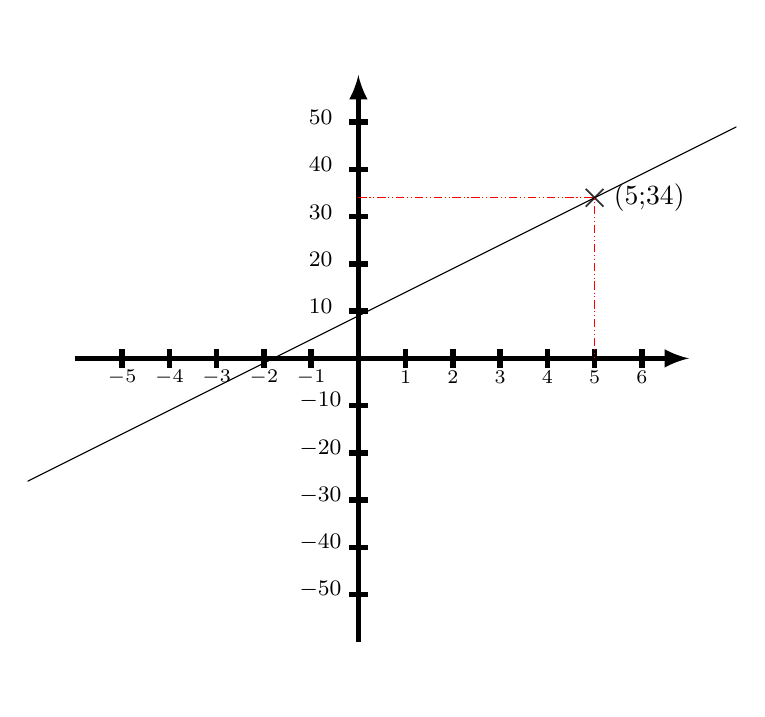
\begin{tikzpicture}[baseline,scale = 0.6]

    \tikzset{
      point/.style={
        thick,
        draw,
        cross out,
        inner sep=0pt,
        minimum width=5pt,
        minimum height=5pt,
      },
    }
    \clip (-7,-7) rectangle (8,7);
    	
	\draw[color ={black},line width = 2,>=latex,->] (-6,0)--(7,0);
	\draw[color ={black},line width = 2,>=latex,->] (0,-6)--(0,6);
	\draw[color ={black},line width = 2] (1,-0.2)--(1,0.2);
	\draw[color ={black},line width = 2] (2,-0.2)--(2,0.2);
	\draw[color ={black},line width = 2] (3,-0.2)--(3,0.2);
	\draw[color ={black},line width = 2] (4,-0.2)--(4,0.2);
	\draw[color ={black},line width = 2] (5,-0.2)--(5,0.2);
	\draw[color ={black},line width = 2] (6,-0.2)--(6,0.2);
	\draw[color ={black},line width = 2] (-1,-0.2)--(-1,0.2);
	\draw[color ={black},line width = 2] (-2,-0.2)--(-2,0.2);
	\draw[color ={black},line width = 2] (-3,-0.2)--(-3,0.2);
	\draw[color ={black},line width = 2] (-4,-0.2)--(-4,0.2);
	\draw[color ={black},line width = 2] (-5,-0.2)--(-5,0.2);
	\draw[color ={black},line width = 2] (-0.2,1)--(0.2,1);
	\draw[color ={black},line width = 2] (-0.2,2)--(0.2,2);
	\draw[color ={black},line width = 2] (-0.2,3)--(0.2,3);
	\draw[color ={black},line width = 2] (-0.2,4)--(0.2,4);
	\draw[color ={black},line width = 2] (-0.2,5)--(0.2,5);
	\draw[color ={black},line width = 2] (-0.2,-1)--(0.2,-1);
	\draw[color ={black},line width = 2] (-0.2,-2)--(0.2,-2);
	\draw[color ={black},line width = 2] (-0.2,-3)--(0.2,-3);
	\draw[color ={black},line width = 2] (-0.2,-4)--(0.2,-4);
	\draw[color ={black},line width = 2] (-0.2,-5)--(0.2,-5);
	\draw (1,-0.4) node[anchor = center] {\scriptsize \color{black}{$1$}};
	\draw (2,-0.4) node[anchor = center] {\scriptsize \color{black}{$2$}};
	\draw (3,-0.4) node[anchor = center] {\scriptsize \color{black}{$3$}};
	\draw (4,-0.4) node[anchor = center] {\scriptsize \color{black}{$4$}};
	\draw (5,-0.4) node[anchor = center] {\scriptsize \color{black}{$5$}};
	\draw (6,-0.4) node[anchor = center] {\scriptsize \color{black}{$6$}};
	\draw (-1,-0.4) node[anchor = center] {\scriptsize \color{black}{$-1$}};
	\draw (-2,-0.4) node[anchor = center] {\scriptsize \color{black}{$-2$}};
	\draw (-3,-0.4) node[anchor = center] {\scriptsize \color{black}{$-3$}};
	\draw (-4,-0.4) node[anchor = center] {\scriptsize \color{black}{$-4$}};
	\draw (-5,-0.4) node[anchor = center] {\scriptsize \color{black}{$-5$}};
	\draw (-0.8,1.1) node[anchor = center] {\footnotesize \color{black}{$10$}};
	\draw (-0.8,2.1) node[anchor = center] {\footnotesize \color{black}{$20$}};
	\draw (-0.8,3.1) node[anchor = center] {\footnotesize \color{black}{$30$}};
	\draw (-0.8,4.1) node[anchor = center] {\footnotesize \color{black}{$40$}};
	\draw (-0.8,5.1) node[anchor = center] {\footnotesize \color{black}{$50$}};
	\draw (-0.8,-0.9) node[anchor = center] {\footnotesize \color{black}{$-10$}};
	\draw (-0.8,-1.9) node[anchor = center] {\footnotesize \color{black}{$-20$}};
	\draw (-0.8,-2.9) node[anchor = center] {\footnotesize \color{black}{$-30$}};
	\draw (-0.8,-3.9) node[anchor = center] {\footnotesize \color{black}{$-40$}};
	\draw (-0.8,-4.9) node[anchor = center] {\footnotesize \color{black}{$-50$}};
	\draw[color={black}] (-44.721359099991595,-21.460679549995803)--(49.721359099991595,25.7606795499958);
	\draw[color ={{black}},line width = 0.625,opacity = 0.8] (4.8125,3.5875000000000004)--(5.1875,3.2125000000000004);\draw[color ={{black}},line width = 0.625,opacity = 0.8] (4.8125,3.2125000000000004)--(5.1875,3.5875000000000004);
	\draw [color={black}] (5.2,3.4) node[anchor = west,scale=1, rotate = 0] {(5;34)};
	\draw[color={red}, densely dash dot dot ] (0,3.4)--(5,3.4)--(5,0);

\end{tikzpicture}\\
	\item Soit $h$ la fonction affine telle que $h(7)=-32$ et $h(0)=-4$.\\Calculer l'image de $3$ par $h$.
	\item Soit $i$ la fonction affine telle que $i(9)=32$ et $i(0)=5$.\\Donner l'expression de  $i(x)$.
	\item La droite représentant la fonction affine $j$ passe par le point de coordonnées $(5;-45)$ et coupe l'axe des ordonnées en $(0;-5)$.\\Calculer l'antécédent de $-61$ par $j$.\\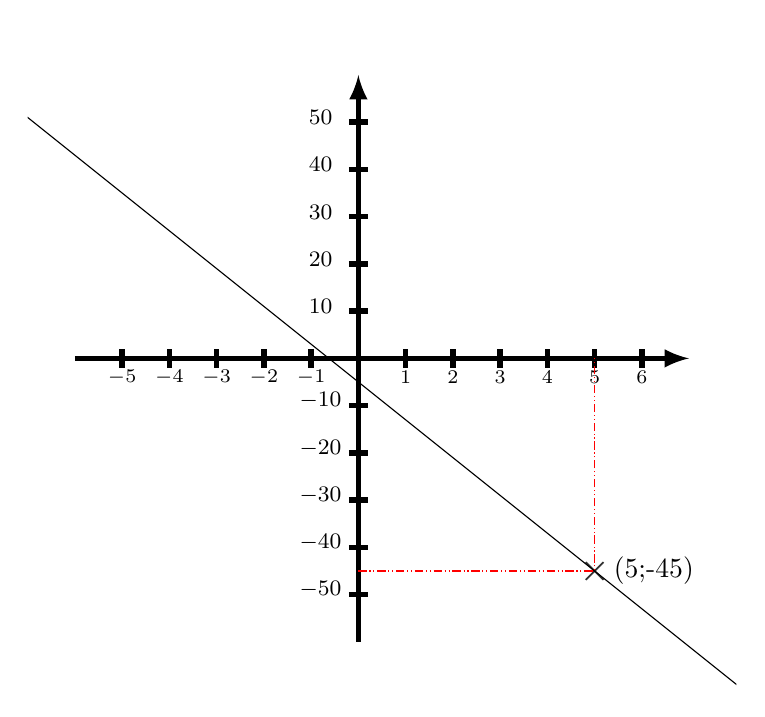
\begin{tikzpicture}[baseline,scale = 0.6]

    \tikzset{
      point/.style={
        thick,
        draw,
        cross out,
        inner sep=0pt,
        minimum width=5pt,
        minimum height=5pt,
      },
    }
    \clip (-7,-7) rectangle (8,7);
    	
	\draw[color ={black},line width = 2,>=latex,->] (-6,0)--(7,0);
	\draw[color ={black},line width = 2,>=latex,->] (0,-6)--(0,6);
	\draw[color ={black},line width = 2] (1,-0.2)--(1,0.2);
	\draw[color ={black},line width = 2] (2,-0.2)--(2,0.2);
	\draw[color ={black},line width = 2] (3,-0.2)--(3,0.2);
	\draw[color ={black},line width = 2] (4,-0.2)--(4,0.2);
	\draw[color ={black},line width = 2] (5,-0.2)--(5,0.2);
	\draw[color ={black},line width = 2] (6,-0.2)--(6,0.2);
	\draw[color ={black},line width = 2] (-1,-0.2)--(-1,0.2);
	\draw[color ={black},line width = 2] (-2,-0.2)--(-2,0.2);
	\draw[color ={black},line width = 2] (-3,-0.2)--(-3,0.2);
	\draw[color ={black},line width = 2] (-4,-0.2)--(-4,0.2);
	\draw[color ={black},line width = 2] (-5,-0.2)--(-5,0.2);
	\draw[color ={black},line width = 2] (-0.2,1)--(0.2,1);
	\draw[color ={black},line width = 2] (-0.2,2)--(0.2,2);
	\draw[color ={black},line width = 2] (-0.2,3)--(0.2,3);
	\draw[color ={black},line width = 2] (-0.2,4)--(0.2,4);
	\draw[color ={black},line width = 2] (-0.2,5)--(0.2,5);
	\draw[color ={black},line width = 2] (-0.2,-1)--(0.2,-1);
	\draw[color ={black},line width = 2] (-0.2,-2)--(0.2,-2);
	\draw[color ={black},line width = 2] (-0.2,-3)--(0.2,-3);
	\draw[color ={black},line width = 2] (-0.2,-4)--(0.2,-4);
	\draw[color ={black},line width = 2] (-0.2,-5)--(0.2,-5);
	\draw (1,-0.4) node[anchor = center] {\scriptsize \color{black}{$1$}};
	\draw (2,-0.4) node[anchor = center] {\scriptsize \color{black}{$2$}};
	\draw (3,-0.4) node[anchor = center] {\scriptsize \color{black}{$3$}};
	\draw (4,-0.4) node[anchor = center] {\scriptsize \color{black}{$4$}};
	\draw (5,-0.4) node[anchor = center] {\scriptsize \color{black}{$5$}};
	\draw (6,-0.4) node[anchor = center] {\scriptsize \color{black}{$6$}};
	\draw (-1,-0.4) node[anchor = center] {\scriptsize \color{black}{$-1$}};
	\draw (-2,-0.4) node[anchor = center] {\scriptsize \color{black}{$-2$}};
	\draw (-3,-0.4) node[anchor = center] {\scriptsize \color{black}{$-3$}};
	\draw (-4,-0.4) node[anchor = center] {\scriptsize \color{black}{$-4$}};
	\draw (-5,-0.4) node[anchor = center] {\scriptsize \color{black}{$-5$}};
	\draw (-0.8,1.1) node[anchor = center] {\footnotesize \color{black}{$10$}};
	\draw (-0.8,2.1) node[anchor = center] {\footnotesize \color{black}{$20$}};
	\draw (-0.8,3.1) node[anchor = center] {\footnotesize \color{black}{$30$}};
	\draw (-0.8,4.1) node[anchor = center] {\footnotesize \color{black}{$40$}};
	\draw (-0.8,5.1) node[anchor = center] {\footnotesize \color{black}{$50$}};
	\draw (-0.8,-0.9) node[anchor = center] {\footnotesize \color{black}{$-10$}};
	\draw (-0.8,-1.9) node[anchor = center] {\footnotesize \color{black}{$-20$}};
	\draw (-0.8,-2.9) node[anchor = center] {\footnotesize \color{black}{$-30$}};
	\draw (-0.8,-3.9) node[anchor = center] {\footnotesize \color{black}{$-40$}};
	\draw (-0.8,-4.9) node[anchor = center] {\footnotesize \color{black}{$-50$}};
	\draw[color={black}] (-39.043441919912844,30.734753535930274)--(44.043441919912844,-35.734753535930274);
	\draw[color ={{black}},line width = 0.625,opacity = 0.8] (4.8125,-4.3125)--(5.1875,-4.6875);\draw[color ={{black}},line width = 0.625,opacity = 0.8] (4.8125,-4.6875)--(5.1875,-4.3125);
	\draw [color={black}] (5.2,-4.5) node[anchor = west,scale=1, rotate = 0] {(5;-45)};
	\draw[color={red}, densely dash dot dot ] (0,-4.5)--(5,-4.5)--(5,0);

\end{tikzpicture}\\
	\item Soit $k$ la fonction affine telle que $k(7)=19$ et $k(0)=-9$.\\Calculer l'antécédent de $-17$.
	\item Soit $l(x)=-6x+2$.\\Calculer l'antécédent de $-10$ par $l$.
	\item La droite représentant la fonction affine $m$ passe par le point de coordonnées $(7;-33)$ et coupe l'axe des ordonnées en $(0;-5)$.\\Calculer l'image de $10$ par $m$.\\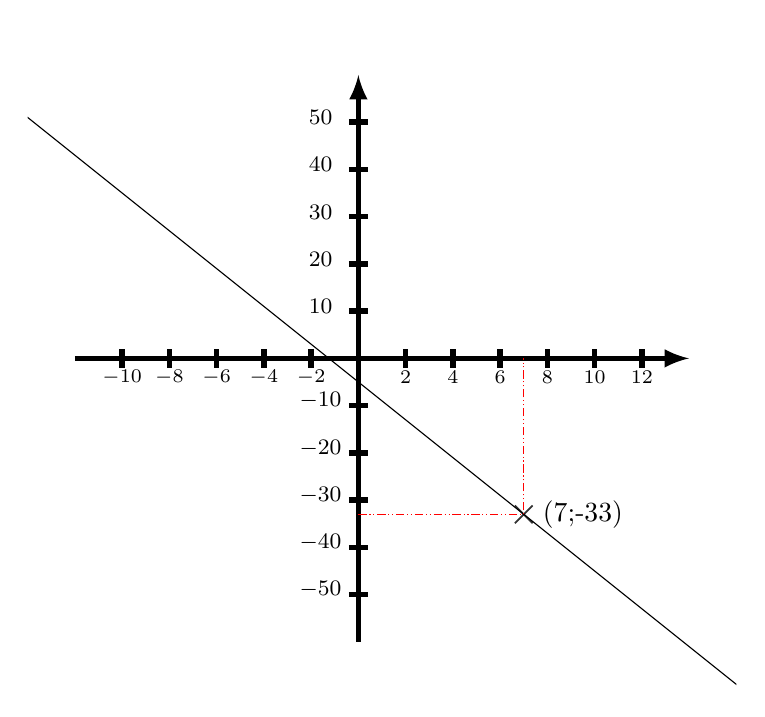
\begin{tikzpicture}[baseline,scale = 0.6]

    \tikzset{
      point/.style={
        thick,
        draw,
        cross out,
        inner sep=0pt,
        minimum width=5pt,
        minimum height=5pt,
      },
    }
    \clip (-7,-7) rectangle (8,7);
    	
	\draw[color ={black},line width = 2,>=latex,->] (-6,0)--(7,0);
	\draw[color ={black},line width = 2,>=latex,->] (0,-6)--(0,6);
	\draw[color ={black},line width = 2] (1,-0.2)--(1,0.2);
	\draw[color ={black},line width = 2] (2,-0.2)--(2,0.2);
	\draw[color ={black},line width = 2] (3,-0.2)--(3,0.2);
	\draw[color ={black},line width = 2] (4,-0.2)--(4,0.2);
	\draw[color ={black},line width = 2] (5,-0.2)--(5,0.2);
	\draw[color ={black},line width = 2] (6,-0.2)--(6,0.2);
	\draw[color ={black},line width = 2] (-1,-0.2)--(-1,0.2);
	\draw[color ={black},line width = 2] (-2,-0.2)--(-2,0.2);
	\draw[color ={black},line width = 2] (-3,-0.2)--(-3,0.2);
	\draw[color ={black},line width = 2] (-4,-0.2)--(-4,0.2);
	\draw[color ={black},line width = 2] (-5,-0.2)--(-5,0.2);
	\draw[color ={black},line width = 2] (-0.2,1)--(0.2,1);
	\draw[color ={black},line width = 2] (-0.2,2)--(0.2,2);
	\draw[color ={black},line width = 2] (-0.2,3)--(0.2,3);
	\draw[color ={black},line width = 2] (-0.2,4)--(0.2,4);
	\draw[color ={black},line width = 2] (-0.2,5)--(0.2,5);
	\draw[color ={black},line width = 2] (-0.2,-1)--(0.2,-1);
	\draw[color ={black},line width = 2] (-0.2,-2)--(0.2,-2);
	\draw[color ={black},line width = 2] (-0.2,-3)--(0.2,-3);
	\draw[color ={black},line width = 2] (-0.2,-4)--(0.2,-4);
	\draw[color ={black},line width = 2] (-0.2,-5)--(0.2,-5);
	\draw (1,-0.4) node[anchor = center] {\scriptsize \color{black}{$2$}};
	\draw (2,-0.4) node[anchor = center] {\scriptsize \color{black}{$4$}};
	\draw (3,-0.4) node[anchor = center] {\scriptsize \color{black}{$6$}};
	\draw (4,-0.4) node[anchor = center] {\scriptsize \color{black}{$8$}};
	\draw (5,-0.4) node[anchor = center] {\scriptsize \color{black}{$10$}};
	\draw (6,-0.4) node[anchor = center] {\scriptsize \color{black}{$12$}};
	\draw (-1,-0.4) node[anchor = center] {\scriptsize \color{black}{$-2$}};
	\draw (-2,-0.4) node[anchor = center] {\scriptsize \color{black}{$-4$}};
	\draw (-3,-0.4) node[anchor = center] {\scriptsize \color{black}{$-6$}};
	\draw (-4,-0.4) node[anchor = center] {\scriptsize \color{black}{$-8$}};
	\draw (-5,-0.4) node[anchor = center] {\scriptsize \color{black}{$-10$}};
	\draw (-0.8,1.1) node[anchor = center] {\footnotesize \color{black}{$10$}};
	\draw (-0.8,2.1) node[anchor = center] {\footnotesize \color{black}{$20$}};
	\draw (-0.8,3.1) node[anchor = center] {\footnotesize \color{black}{$30$}};
	\draw (-0.8,4.1) node[anchor = center] {\footnotesize \color{black}{$40$}};
	\draw (-0.8,5.1) node[anchor = center] {\footnotesize \color{black}{$50$}};
	\draw (-0.8,-0.9) node[anchor = center] {\footnotesize \color{black}{$-10$}};
	\draw (-0.8,-1.9) node[anchor = center] {\footnotesize \color{black}{$-20$}};
	\draw (-0.8,-2.9) node[anchor = center] {\footnotesize \color{black}{$-30$}};
	\draw (-0.8,-3.9) node[anchor = center] {\footnotesize \color{black}{$-40$}};
	\draw (-0.8,-4.9) node[anchor = center] {\footnotesize \color{black}{$-50$}};
	\draw[color={black}] (-39.043440177752515,30.734752142202016)--(42.543440177752515,-34.53475214220202);
	\draw[color ={{black}},line width = 0.625,opacity = 0.8] (3.3125,-3.1125000000000003)--(3.6875,-3.4875000000000003);\draw[color ={{black}},line width = 0.625,opacity = 0.8] (3.3125,-3.4875000000000003)--(3.6875,-3.1125000000000003);
	\draw [color={black}] (3.7,-3.3) node[anchor = west,scale=1, rotate = 0] {(7;-33)};
	\draw[color={red}, densely dash dot dot ] (0,-3.3)--(3.5,-3.3)--(3.5,0);

\end{tikzpicture}\\
\end{enumerate}
\end{EXO}

% @see : https://coopmaths.fr/alea?uuid=b4c0d&id=11FA8-9&n=1&d=10&s=1&s2=3&alea=ub6j&cd=1&cols=1
\begin{EXO}{}{11FA8-9}


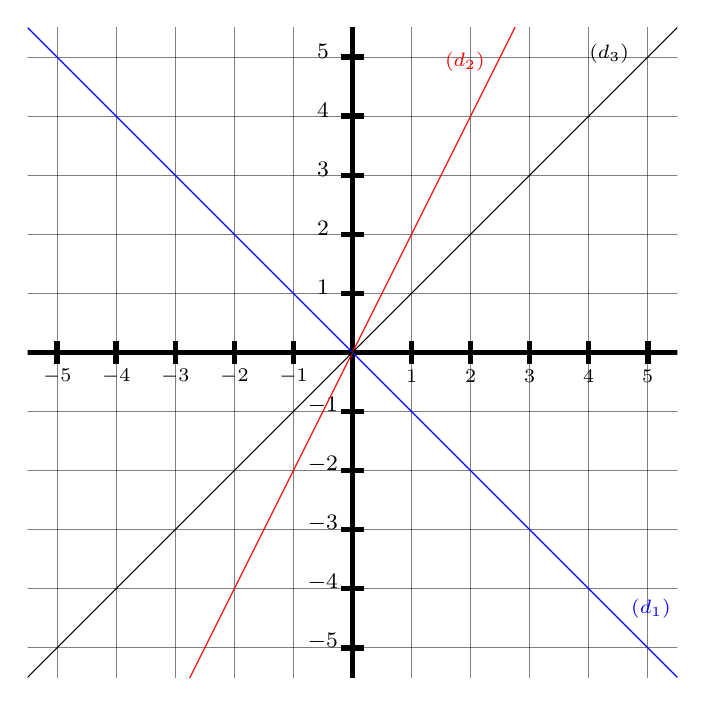
\begin{tikzpicture}[baseline,scale = 0.75]

    \tikzset{
      point/.style={
        thick,
        draw,
        cross out,
        inner sep=0pt,
        minimum width=5pt,
        minimum height=5pt,
      },
    }
    \clip (-5.5,-5.5) rectangle (5.5,5.5);
    	
	\draw[color ={black},line width = 2,>=latex,->] (-6,0)--(6,0);
	\draw[color ={black},line width = 2,>=latex,->] (0,-6)--(0,6);
	\draw[color ={black},opacity = 0.5] (-6,1)--(6,1);
	\draw[color ={black},opacity = 0.5] (-6,2)--(6,2);
	\draw[color ={black},opacity = 0.5] (-6,3)--(6,3);
	\draw[color ={black},opacity = 0.5] (-6,4)--(6,4);
	\draw[color ={black},opacity = 0.5] (-6,5)--(6,5);
	\draw[color ={black},opacity = 0.5] (-6,6)--(6,6);
	\draw[color ={black},opacity = 0.5] (-6,-1)--(6,-1);
	\draw[color ={black},opacity = 0.5] (-6,-2)--(6,-2);
	\draw[color ={black},opacity = 0.5] (-6,-3)--(6,-3);
	\draw[color ={black},opacity = 0.5] (-6,-4)--(6,-4);
	\draw[color ={black},opacity = 0.5] (-6,-5)--(6,-5);
	\draw[color ={black},opacity = 0.5] (-6,-6)--(6,-6);
	\draw[color ={black},opacity = 0.5] (1,-6)--(1,6);
	\draw[color ={black},opacity = 0.5] (2,-6)--(2,6);
	\draw[color ={black},opacity = 0.5] (3,-6)--(3,6);
	\draw[color ={black},opacity = 0.5] (4,-6)--(4,6);
	\draw[color ={black},opacity = 0.5] (5,-6)--(5,6);
	\draw[color ={black},opacity = 0.5] (6,-6)--(6,6);
	\draw[color ={black},opacity = 0.5] (-1,-6)--(-1,6);
	\draw[color ={black},opacity = 0.5] (-2,-6)--(-2,6);
	\draw[color ={black},opacity = 0.5] (-3,-6)--(-3,6);
	\draw[color ={black},opacity = 0.5] (-4,-6)--(-4,6);
	\draw[color ={black},opacity = 0.5] (-5,-6)--(-5,6);
	\draw[color ={black},opacity = 0.5] (-6,-6)--(-6,6);
	\draw[color ={black},line width = 2] (1,-0.2)--(1,0.2);
	\draw[color ={black},line width = 2] (2,-0.2)--(2,0.2);
	\draw[color ={black},line width = 2] (3,-0.2)--(3,0.2);
	\draw[color ={black},line width = 2] (4,-0.2)--(4,0.2);
	\draw[color ={black},line width = 2] (5,-0.2)--(5,0.2);
	\draw[color ={black},line width = 2] (-1,-0.2)--(-1,0.2);
	\draw[color ={black},line width = 2] (-2,-0.2)--(-2,0.2);
	\draw[color ={black},line width = 2] (-3,-0.2)--(-3,0.2);
	\draw[color ={black},line width = 2] (-4,-0.2)--(-4,0.2);
	\draw[color ={black},line width = 2] (-5,-0.2)--(-5,0.2);
	\draw[color ={black},line width = 2] (-0.2,1)--(0.2,1);
	\draw[color ={black},line width = 2] (-0.2,2)--(0.2,2);
	\draw[color ={black},line width = 2] (-0.2,3)--(0.2,3);
	\draw[color ={black},line width = 2] (-0.2,4)--(0.2,4);
	\draw[color ={black},line width = 2] (-0.2,5)--(0.2,5);
	\draw[color ={black},line width = 2] (-0.2,-1)--(0.2,-1);
	\draw[color ={black},line width = 2] (-0.2,-2)--(0.2,-2);
	\draw[color ={black},line width = 2] (-0.2,-3)--(0.2,-3);
	\draw[color ={black},line width = 2] (-0.2,-4)--(0.2,-4);
	\draw[color ={black},line width = 2] (-0.2,-5)--(0.2,-5);
	\draw (1,-0.4) node[anchor = center] {\scriptsize \color{black}{$1$}};
	\draw (2,-0.4) node[anchor = center] {\scriptsize \color{black}{$2$}};
	\draw (3,-0.4) node[anchor = center] {\scriptsize \color{black}{$3$}};
	\draw (4,-0.4) node[anchor = center] {\scriptsize \color{black}{$4$}};
	\draw (5,-0.4) node[anchor = center] {\scriptsize \color{black}{$5$}};
	\draw (-1,-0.4) node[anchor = center] {\scriptsize \color{black}{$-1$}};
	\draw (-2,-0.4) node[anchor = center] {\scriptsize \color{black}{$-2$}};
	\draw (-3,-0.4) node[anchor = center] {\scriptsize \color{black}{$-3$}};
	\draw (-4,-0.4) node[anchor = center] {\scriptsize \color{black}{$-4$}};
	\draw (-5,-0.4) node[anchor = center] {\scriptsize \color{black}{$-5$}};
	\draw (-0.5,1.1) node[anchor = center] {\footnotesize \color{black}{$1$}};
	\draw (-0.5,2.1) node[anchor = center] {\footnotesize \color{black}{$2$}};
	\draw (-0.5,3.1) node[anchor = center] {\footnotesize \color{black}{$3$}};
	\draw (-0.5,4.1) node[anchor = center] {\footnotesize \color{black}{$4$}};
	\draw (-0.5,5.1) node[anchor = center] {\footnotesize \color{black}{$5$}};
	\draw (-0.5,-0.9) node[anchor = center] {\footnotesize \color{black}{$-1$}};
	\draw (-0.5,-1.9) node[anchor = center] {\footnotesize \color{black}{$-2$}};
	\draw (-0.5,-2.9) node[anchor = center] {\footnotesize \color{black}{$-3$}};
	\draw (-0.5,-3.9) node[anchor = center] {\footnotesize \color{black}{$-4$}};
	\draw (-0.5,-4.9) node[anchor = center] {\footnotesize \color{black}{$-5$}};
	\draw[color={blue}] (-35.355328118658136,35.355328118658136)--(36.355328118658136,-36.355328118658136);
	\draw (5.053553390593274,-4.346446609406726) node[anchor = center] {\scriptsize \color{blue}{$(d_1)$}};
	\draw[color={red}] (-22.360679549995798,-44.721359099991595)--(23.360679549995798,46.721359099991595);
	\draw (1.9027864045000422,4.923606797749979) node[anchor = center] {\scriptsize \color{red}{$(d_2)$}};
	\draw[color={black}] (-35.355328118658136,-35.355328118658136)--(36.355328118658136,36.355328118658136);
	\draw (4.346446609406726,5.053553390593274) node[anchor = center] {\scriptsize \color{black}{$(d_3)$}};

\end{tikzpicture}\\
\begin{enumerate}[]
	\item Déterminer l'expression de la fonction $f_1$ représentée par la droite $(d_1)$.
	\item Déterminer l'expression de la fonction $f_2$ représentée par la droite $(d_2)$.
	\item Déterminer l'expression de la fonction $f_3$ représentée par la droite $(d_3)$.
\end{enumerate}
\end{EXO}

% @see : https://coopmaths.fr/alea?uuid=ef897&id=11FA8-11&n=3&d=10&s=1&alea=957J&cd=1&cols=1
\begin{EXO}{}{11FA8-11}


\begin{enumerate}[]
	\item  Déterminer l'expression algébrique de la fonction affine $f$ définie sur $\mathbb R$, sachant que
                        $f(5)=29$ et que $f(3)=17$.\\
	\item  Déterminer l'expression algébrique de la fonction affine $f$ définie sur $\mathbb R$, sachant que
                        $f(5)=17$ et que $f(6)=20$.\\
	\item  Déterminer l'expression algébrique de la fonction affine $f$ définie sur $\mathbb R$, sachant que
                        $f(2)=1$ et que $f(7)=-4$.\\
\end{enumerate}
\end{EXO}

% @see : https://coopmaths.fr/alea?uuid=056fa&id=11FA8-12&n=2&d=10&s=3&s2=3&s3=3&s4=2&alea=fwEB&cd=1&cols=1
\begin{EXO}{}{11FA8-12}


\begin{enumerate}[]
	\item On a représenté ci-dessous une fonction affine $g$.

\medskip
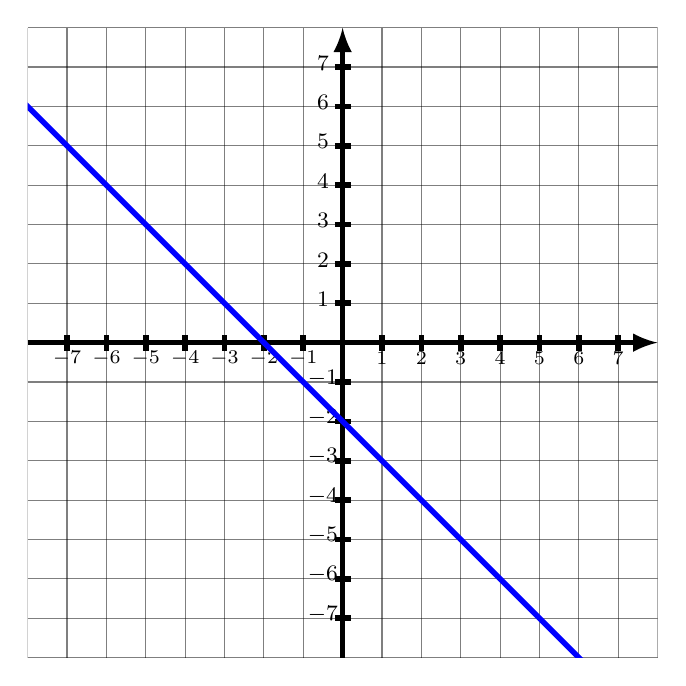
\begin{tikzpicture}[baseline,scale = 0.5]

    \tikzset{
      point/.style={
        thick,
        draw,
        cross out,
        inner sep=0pt,
        minimum width=5pt,
        minimum height=5pt,
      },
    }
    \clip (-8,-8) rectangle (8,8);
    	
	\draw[color ={black},line width = 2,>=latex,->] (-8,0)--(8,0);
	\draw[color ={black},line width = 2,>=latex,->] (0,-8)--(0,8);
	\draw[color ={black},opacity = 0.5] (-8,1)--(8,1);
	\draw[color ={black},opacity = 0.5] (-8,2)--(8,2);
	\draw[color ={black},opacity = 0.5] (-8,3)--(8,3);
	\draw[color ={black},opacity = 0.5] (-8,4)--(8,4);
	\draw[color ={black},opacity = 0.5] (-8,5)--(8,5);
	\draw[color ={black},opacity = 0.5] (-8,6)--(8,6);
	\draw[color ={black},opacity = 0.5] (-8,7)--(8,7);
	\draw[color ={black},opacity = 0.5] (-8,8)--(8,8);
	\draw[color ={black},opacity = 0.5] (-8,-1)--(8,-1);
	\draw[color ={black},opacity = 0.5] (-8,-2)--(8,-2);
	\draw[color ={black},opacity = 0.5] (-8,-3)--(8,-3);
	\draw[color ={black},opacity = 0.5] (-8,-4)--(8,-4);
	\draw[color ={black},opacity = 0.5] (-8,-5)--(8,-5);
	\draw[color ={black},opacity = 0.5] (-8,-6)--(8,-6);
	\draw[color ={black},opacity = 0.5] (-8,-7)--(8,-7);
	\draw[color ={black},opacity = 0.5] (-8,-8)--(8,-8);
	\draw[color ={black},opacity = 0.5] (1,-8)--(1,8);
	\draw[color ={black},opacity = 0.5] (2,-8)--(2,8);
	\draw[color ={black},opacity = 0.5] (3,-8)--(3,8);
	\draw[color ={black},opacity = 0.5] (4,-8)--(4,8);
	\draw[color ={black},opacity = 0.5] (5,-8)--(5,8);
	\draw[color ={black},opacity = 0.5] (6,-8)--(6,8);
	\draw[color ={black},opacity = 0.5] (7,-8)--(7,8);
	\draw[color ={black},opacity = 0.5] (8,-8)--(8,8);
	\draw[color ={black},opacity = 0.5] (-1,-8)--(-1,8);
	\draw[color ={black},opacity = 0.5] (-2,-8)--(-2,8);
	\draw[color ={black},opacity = 0.5] (-3,-8)--(-3,8);
	\draw[color ={black},opacity = 0.5] (-4,-8)--(-4,8);
	\draw[color ={black},opacity = 0.5] (-5,-8)--(-5,8);
	\draw[color ={black},opacity = 0.5] (-6,-8)--(-6,8);
	\draw[color ={black},opacity = 0.5] (-7,-8)--(-7,8);
	\draw[color ={black},opacity = 0.5] (-8,-8)--(-8,8);
	\draw[color ={black},line width = 2] (1,-0.2)--(1,0.2);
	\draw[color ={black},line width = 2] (2,-0.2)--(2,0.2);
	\draw[color ={black},line width = 2] (3,-0.2)--(3,0.2);
	\draw[color ={black},line width = 2] (4,-0.2)--(4,0.2);
	\draw[color ={black},line width = 2] (5,-0.2)--(5,0.2);
	\draw[color ={black},line width = 2] (6,-0.2)--(6,0.2);
	\draw[color ={black},line width = 2] (7,-0.2)--(7,0.2);
	\draw[color ={black},line width = 2] (-1,-0.2)--(-1,0.2);
	\draw[color ={black},line width = 2] (-2,-0.2)--(-2,0.2);
	\draw[color ={black},line width = 2] (-3,-0.2)--(-3,0.2);
	\draw[color ={black},line width = 2] (-4,-0.2)--(-4,0.2);
	\draw[color ={black},line width = 2] (-5,-0.2)--(-5,0.2);
	\draw[color ={black},line width = 2] (-6,-0.2)--(-6,0.2);
	\draw[color ={black},line width = 2] (-7,-0.2)--(-7,0.2);
	\draw[color ={black},line width = 2] (-0.2,1)--(0.2,1);
	\draw[color ={black},line width = 2] (-0.2,2)--(0.2,2);
	\draw[color ={black},line width = 2] (-0.2,3)--(0.2,3);
	\draw[color ={black},line width = 2] (-0.2,4)--(0.2,4);
	\draw[color ={black},line width = 2] (-0.2,5)--(0.2,5);
	\draw[color ={black},line width = 2] (-0.2,6)--(0.2,6);
	\draw[color ={black},line width = 2] (-0.2,7)--(0.2,7);
	\draw[color ={black},line width = 2] (-0.2,-1)--(0.2,-1);
	\draw[color ={black},line width = 2] (-0.2,-2)--(0.2,-2);
	\draw[color ={black},line width = 2] (-0.2,-3)--(0.2,-3);
	\draw[color ={black},line width = 2] (-0.2,-4)--(0.2,-4);
	\draw[color ={black},line width = 2] (-0.2,-5)--(0.2,-5);
	\draw[color ={black},line width = 2] (-0.2,-6)--(0.2,-6);
	\draw[color ={black},line width = 2] (-0.2,-7)--(0.2,-7);
	\draw (1,-0.4) node[anchor = center] {\scriptsize \color{black}{$1$}};
	\draw (2,-0.4) node[anchor = center] {\scriptsize \color{black}{$2$}};
	\draw (3,-0.4) node[anchor = center] {\scriptsize \color{black}{$3$}};
	\draw (4,-0.4) node[anchor = center] {\scriptsize \color{black}{$4$}};
	\draw (5,-0.4) node[anchor = center] {\scriptsize \color{black}{$5$}};
	\draw (6,-0.4) node[anchor = center] {\scriptsize \color{black}{$6$}};
	\draw (7,-0.4) node[anchor = center] {\scriptsize \color{black}{$7$}};
	\draw (-1,-0.4) node[anchor = center] {\scriptsize \color{black}{$-1$}};
	\draw (-2,-0.4) node[anchor = center] {\scriptsize \color{black}{$-2$}};
	\draw (-3,-0.4) node[anchor = center] {\scriptsize \color{black}{$-3$}};
	\draw (-4,-0.4) node[anchor = center] {\scriptsize \color{black}{$-4$}};
	\draw (-5,-0.4) node[anchor = center] {\scriptsize \color{black}{$-5$}};
	\draw (-6,-0.4) node[anchor = center] {\scriptsize \color{black}{$-6$}};
	\draw (-7,-0.4) node[anchor = center] {\scriptsize \color{black}{$-7$}};
	\draw (-0.5,1.1) node[anchor = center] {\footnotesize \color{black}{$1$}};
	\draw (-0.5,2.1) node[anchor = center] {\footnotesize \color{black}{$2$}};
	\draw (-0.5,3.1) node[anchor = center] {\footnotesize \color{black}{$3$}};
	\draw (-0.5,4.1) node[anchor = center] {\footnotesize \color{black}{$4$}};
	\draw (-0.5,5.1) node[anchor = center] {\footnotesize \color{black}{$5$}};
	\draw (-0.5,6.1) node[anchor = center] {\footnotesize \color{black}{$6$}};
	\draw (-0.5,7.1) node[anchor = center] {\footnotesize \color{black}{$7$}};
	\draw (-0.5,-0.9) node[anchor = center] {\footnotesize \color{black}{$-1$}};
	\draw (-0.5,-1.9) node[anchor = center] {\footnotesize \color{black}{$-2$}};
	\draw (-0.5,-2.9) node[anchor = center] {\footnotesize \color{black}{$-3$}};
	\draw (-0.5,-3.9) node[anchor = center] {\footnotesize \color{black}{$-4$}};
	\draw (-0.5,-4.9) node[anchor = center] {\footnotesize \color{black}{$-5$}};
	\draw (-0.5,-5.9) node[anchor = center] {\footnotesize \color{black}{$-6$}};
	\draw (-0.5,-6.9) node[anchor = center] {\footnotesize \color{black}{$-7$}};
	\draw[color={blue},line width = 2] (-35.355328118658136,33.355328118658136)--(36.355328118658136,-38.355328118658136);

\end{tikzpicture}\\\\\textbf {a.} Quelle est l'ordonnée à l'origine de la fonction $g$ ?\\\textbf {b.} Quel est le coefficient directeur de $g$ ?\\\textbf {c.} En déduire l'expression algébrique de $g$.
	\item On a représenté ci-dessous une fonction affine $f_3$.

\medskip
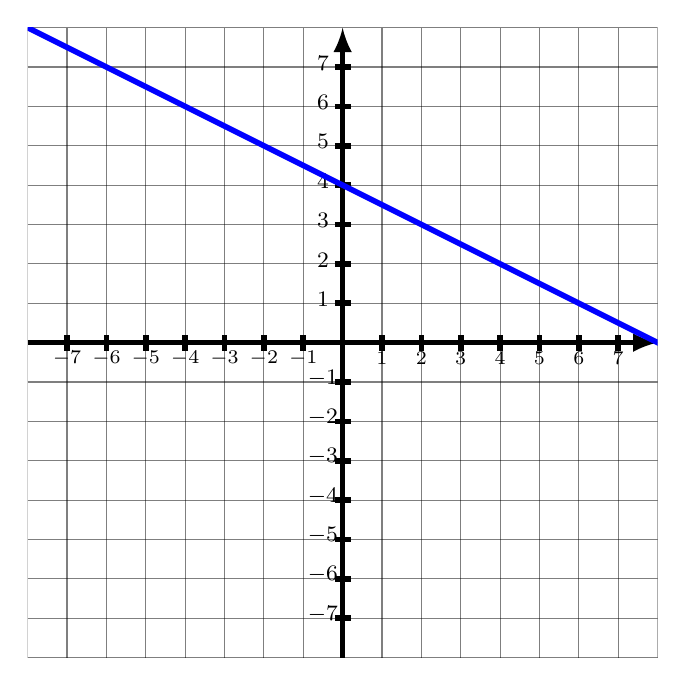
\begin{tikzpicture}[baseline,scale = 0.5]

    \tikzset{
      point/.style={
        thick,
        draw,
        cross out,
        inner sep=0pt,
        minimum width=5pt,
        minimum height=5pt,
      },
    }
    \clip (-8,-8) rectangle (8,8);
    	
	\draw[color ={black},line width = 2,>=latex,->] (-8,0)--(8,0);
	\draw[color ={black},line width = 2,>=latex,->] (0,-8)--(0,8);
	\draw[color ={black},opacity = 0.5] (-8,1)--(8,1);
	\draw[color ={black},opacity = 0.5] (-8,2)--(8,2);
	\draw[color ={black},opacity = 0.5] (-8,3)--(8,3);
	\draw[color ={black},opacity = 0.5] (-8,4)--(8,4);
	\draw[color ={black},opacity = 0.5] (-8,5)--(8,5);
	\draw[color ={black},opacity = 0.5] (-8,6)--(8,6);
	\draw[color ={black},opacity = 0.5] (-8,7)--(8,7);
	\draw[color ={black},opacity = 0.5] (-8,8)--(8,8);
	\draw[color ={black},opacity = 0.5] (-8,-1)--(8,-1);
	\draw[color ={black},opacity = 0.5] (-8,-2)--(8,-2);
	\draw[color ={black},opacity = 0.5] (-8,-3)--(8,-3);
	\draw[color ={black},opacity = 0.5] (-8,-4)--(8,-4);
	\draw[color ={black},opacity = 0.5] (-8,-5)--(8,-5);
	\draw[color ={black},opacity = 0.5] (-8,-6)--(8,-6);
	\draw[color ={black},opacity = 0.5] (-8,-7)--(8,-7);
	\draw[color ={black},opacity = 0.5] (-8,-8)--(8,-8);
	\draw[color ={black},opacity = 0.5] (1,-8)--(1,8);
	\draw[color ={black},opacity = 0.5] (2,-8)--(2,8);
	\draw[color ={black},opacity = 0.5] (3,-8)--(3,8);
	\draw[color ={black},opacity = 0.5] (4,-8)--(4,8);
	\draw[color ={black},opacity = 0.5] (5,-8)--(5,8);
	\draw[color ={black},opacity = 0.5] (6,-8)--(6,8);
	\draw[color ={black},opacity = 0.5] (7,-8)--(7,8);
	\draw[color ={black},opacity = 0.5] (8,-8)--(8,8);
	\draw[color ={black},opacity = 0.5] (-1,-8)--(-1,8);
	\draw[color ={black},opacity = 0.5] (-2,-8)--(-2,8);
	\draw[color ={black},opacity = 0.5] (-3,-8)--(-3,8);
	\draw[color ={black},opacity = 0.5] (-4,-8)--(-4,8);
	\draw[color ={black},opacity = 0.5] (-5,-8)--(-5,8);
	\draw[color ={black},opacity = 0.5] (-6,-8)--(-6,8);
	\draw[color ={black},opacity = 0.5] (-7,-8)--(-7,8);
	\draw[color ={black},opacity = 0.5] (-8,-8)--(-8,8);
	\draw[color ={black},line width = 2] (1,-0.2)--(1,0.2);
	\draw[color ={black},line width = 2] (2,-0.2)--(2,0.2);
	\draw[color ={black},line width = 2] (3,-0.2)--(3,0.2);
	\draw[color ={black},line width = 2] (4,-0.2)--(4,0.2);
	\draw[color ={black},line width = 2] (5,-0.2)--(5,0.2);
	\draw[color ={black},line width = 2] (6,-0.2)--(6,0.2);
	\draw[color ={black},line width = 2] (7,-0.2)--(7,0.2);
	\draw[color ={black},line width = 2] (-1,-0.2)--(-1,0.2);
	\draw[color ={black},line width = 2] (-2,-0.2)--(-2,0.2);
	\draw[color ={black},line width = 2] (-3,-0.2)--(-3,0.2);
	\draw[color ={black},line width = 2] (-4,-0.2)--(-4,0.2);
	\draw[color ={black},line width = 2] (-5,-0.2)--(-5,0.2);
	\draw[color ={black},line width = 2] (-6,-0.2)--(-6,0.2);
	\draw[color ={black},line width = 2] (-7,-0.2)--(-7,0.2);
	\draw[color ={black},line width = 2] (-0.2,1)--(0.2,1);
	\draw[color ={black},line width = 2] (-0.2,2)--(0.2,2);
	\draw[color ={black},line width = 2] (-0.2,3)--(0.2,3);
	\draw[color ={black},line width = 2] (-0.2,4)--(0.2,4);
	\draw[color ={black},line width = 2] (-0.2,5)--(0.2,5);
	\draw[color ={black},line width = 2] (-0.2,6)--(0.2,6);
	\draw[color ={black},line width = 2] (-0.2,7)--(0.2,7);
	\draw[color ={black},line width = 2] (-0.2,-1)--(0.2,-1);
	\draw[color ={black},line width = 2] (-0.2,-2)--(0.2,-2);
	\draw[color ={black},line width = 2] (-0.2,-3)--(0.2,-3);
	\draw[color ={black},line width = 2] (-0.2,-4)--(0.2,-4);
	\draw[color ={black},line width = 2] (-0.2,-5)--(0.2,-5);
	\draw[color ={black},line width = 2] (-0.2,-6)--(0.2,-6);
	\draw[color ={black},line width = 2] (-0.2,-7)--(0.2,-7);
	\draw (1,-0.4) node[anchor = center] {\scriptsize \color{black}{$1$}};
	\draw (2,-0.4) node[anchor = center] {\scriptsize \color{black}{$2$}};
	\draw (3,-0.4) node[anchor = center] {\scriptsize \color{black}{$3$}};
	\draw (4,-0.4) node[anchor = center] {\scriptsize \color{black}{$4$}};
	\draw (5,-0.4) node[anchor = center] {\scriptsize \color{black}{$5$}};
	\draw (6,-0.4) node[anchor = center] {\scriptsize \color{black}{$6$}};
	\draw (7,-0.4) node[anchor = center] {\scriptsize \color{black}{$7$}};
	\draw (-1,-0.4) node[anchor = center] {\scriptsize \color{black}{$-1$}};
	\draw (-2,-0.4) node[anchor = center] {\scriptsize \color{black}{$-2$}};
	\draw (-3,-0.4) node[anchor = center] {\scriptsize \color{black}{$-3$}};
	\draw (-4,-0.4) node[anchor = center] {\scriptsize \color{black}{$-4$}};
	\draw (-5,-0.4) node[anchor = center] {\scriptsize \color{black}{$-5$}};
	\draw (-6,-0.4) node[anchor = center] {\scriptsize \color{black}{$-6$}};
	\draw (-7,-0.4) node[anchor = center] {\scriptsize \color{black}{$-7$}};
	\draw (-0.5,1.1) node[anchor = center] {\footnotesize \color{black}{$1$}};
	\draw (-0.5,2.1) node[anchor = center] {\footnotesize \color{black}{$2$}};
	\draw (-0.5,3.1) node[anchor = center] {\footnotesize \color{black}{$3$}};
	\draw (-0.5,4.1) node[anchor = center] {\footnotesize \color{black}{$4$}};
	\draw (-0.5,5.1) node[anchor = center] {\footnotesize \color{black}{$5$}};
	\draw (-0.5,6.1) node[anchor = center] {\footnotesize \color{black}{$6$}};
	\draw (-0.5,7.1) node[anchor = center] {\footnotesize \color{black}{$7$}};
	\draw (-0.5,-0.9) node[anchor = center] {\footnotesize \color{black}{$-1$}};
	\draw (-0.5,-1.9) node[anchor = center] {\footnotesize \color{black}{$-2$}};
	\draw (-0.5,-2.9) node[anchor = center] {\footnotesize \color{black}{$-3$}};
	\draw (-0.5,-3.9) node[anchor = center] {\footnotesize \color{black}{$-4$}};
	\draw (-0.5,-4.9) node[anchor = center] {\footnotesize \color{black}{$-5$}};
	\draw (-0.5,-5.9) node[anchor = center] {\footnotesize \color{black}{$-6$}};
	\draw (-0.5,-6.9) node[anchor = center] {\footnotesize \color{black}{$-7$}};
	\draw[color={blue},line width = 2] (-44.721359099991595,26.360679549995798)--(45.721359099991595,-18.860679549995798);

\end{tikzpicture}\\\\\textbf {a.} Quelle est l'ordonnée à l'origine de la fonction $f_3$ ?\\\textbf {b.} Quel est le coefficient directeur de $f_3$ ?\\\textbf {c.} En déduire l'expression algébrique de $f_3$.
\end{enumerate}
\end{EXO}

% @see : https://coopmaths.fr/alea?uuid=ef897&id=11FA8-11&n=3&d=10&s=1&alea=Aoc4&cd=1&cols=1
\begin{EXO}{}{11FA8-11}


\begin{enumerate}[]
	\item  Déterminer l'expression algébrique de la fonction affine $f$ définie sur $\mathbb R$, sachant que
                        $f(4)=27$ et que $f(7)=42$.\\
	\item  Déterminer l'expression algébrique de la fonction affine $f$ définie sur $\mathbb R$, sachant que
                        $f(3)=-15$ et que $f(9)=-33$.\\
	\item  Déterminer l'expression algébrique de la fonction affine $f$ définie sur $\mathbb R$, sachant que
                        $f(6)=16$ et que $f(9)=25$.\\
\end{enumerate}
\end{EXO}

% @see : https://coopmaths.fr/alea?uuid=e5ddd&id=11FA8-10&n=1&d=10&s=1&s2=3&alea=LiFT&cd=1&cols=1
\begin{EXO}{}{11FA8-10}


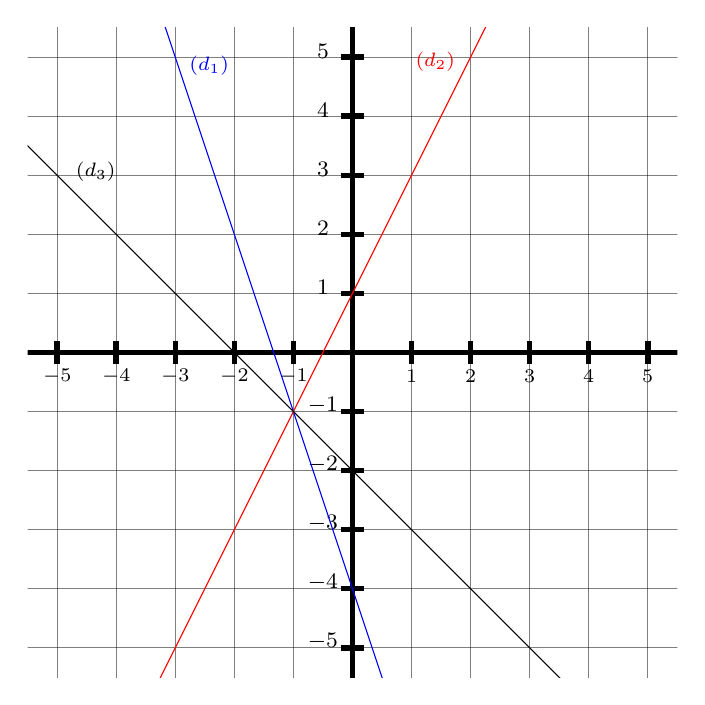
\begin{tikzpicture}[baseline,scale = 0.75]

    \tikzset{
      point/.style={
        thick,
        draw,
        cross out,
        inner sep=0pt,
        minimum width=5pt,
        minimum height=5pt,
      },
    }
    \clip (-5.5,-5.5) rectangle (5.5,5.5);
    	
	\draw[color ={black},line width = 2,>=latex,->] (-6,0)--(6,0);
	\draw[color ={black},line width = 2,>=latex,->] (0,-6)--(0,6);
	\draw[color ={black},opacity = 0.5] (-6,1)--(6,1);
	\draw[color ={black},opacity = 0.5] (-6,2)--(6,2);
	\draw[color ={black},opacity = 0.5] (-6,3)--(6,3);
	\draw[color ={black},opacity = 0.5] (-6,4)--(6,4);
	\draw[color ={black},opacity = 0.5] (-6,5)--(6,5);
	\draw[color ={black},opacity = 0.5] (-6,6)--(6,6);
	\draw[color ={black},opacity = 0.5] (-6,-1)--(6,-1);
	\draw[color ={black},opacity = 0.5] (-6,-2)--(6,-2);
	\draw[color ={black},opacity = 0.5] (-6,-3)--(6,-3);
	\draw[color ={black},opacity = 0.5] (-6,-4)--(6,-4);
	\draw[color ={black},opacity = 0.5] (-6,-5)--(6,-5);
	\draw[color ={black},opacity = 0.5] (-6,-6)--(6,-6);
	\draw[color ={black},opacity = 0.5] (1,-6)--(1,6);
	\draw[color ={black},opacity = 0.5] (2,-6)--(2,6);
	\draw[color ={black},opacity = 0.5] (3,-6)--(3,6);
	\draw[color ={black},opacity = 0.5] (4,-6)--(4,6);
	\draw[color ={black},opacity = 0.5] (5,-6)--(5,6);
	\draw[color ={black},opacity = 0.5] (6,-6)--(6,6);
	\draw[color ={black},opacity = 0.5] (-1,-6)--(-1,6);
	\draw[color ={black},opacity = 0.5] (-2,-6)--(-2,6);
	\draw[color ={black},opacity = 0.5] (-3,-6)--(-3,6);
	\draw[color ={black},opacity = 0.5] (-4,-6)--(-4,6);
	\draw[color ={black},opacity = 0.5] (-5,-6)--(-5,6);
	\draw[color ={black},opacity = 0.5] (-6,-6)--(-6,6);
	\draw[color ={black},line width = 2] (1,-0.2)--(1,0.2);
	\draw[color ={black},line width = 2] (2,-0.2)--(2,0.2);
	\draw[color ={black},line width = 2] (3,-0.2)--(3,0.2);
	\draw[color ={black},line width = 2] (4,-0.2)--(4,0.2);
	\draw[color ={black},line width = 2] (5,-0.2)--(5,0.2);
	\draw[color ={black},line width = 2] (-1,-0.2)--(-1,0.2);
	\draw[color ={black},line width = 2] (-2,-0.2)--(-2,0.2);
	\draw[color ={black},line width = 2] (-3,-0.2)--(-3,0.2);
	\draw[color ={black},line width = 2] (-4,-0.2)--(-4,0.2);
	\draw[color ={black},line width = 2] (-5,-0.2)--(-5,0.2);
	\draw[color ={black},line width = 2] (-0.2,1)--(0.2,1);
	\draw[color ={black},line width = 2] (-0.2,2)--(0.2,2);
	\draw[color ={black},line width = 2] (-0.2,3)--(0.2,3);
	\draw[color ={black},line width = 2] (-0.2,4)--(0.2,4);
	\draw[color ={black},line width = 2] (-0.2,5)--(0.2,5);
	\draw[color ={black},line width = 2] (-0.2,-1)--(0.2,-1);
	\draw[color ={black},line width = 2] (-0.2,-2)--(0.2,-2);
	\draw[color ={black},line width = 2] (-0.2,-3)--(0.2,-3);
	\draw[color ={black},line width = 2] (-0.2,-4)--(0.2,-4);
	\draw[color ={black},line width = 2] (-0.2,-5)--(0.2,-5);
	\draw (1,-0.4) node[anchor = center] {\scriptsize \color{black}{$1$}};
	\draw (2,-0.4) node[anchor = center] {\scriptsize \color{black}{$2$}};
	\draw (3,-0.4) node[anchor = center] {\scriptsize \color{black}{$3$}};
	\draw (4,-0.4) node[anchor = center] {\scriptsize \color{black}{$4$}};
	\draw (5,-0.4) node[anchor = center] {\scriptsize \color{black}{$5$}};
	\draw (-1,-0.4) node[anchor = center] {\scriptsize \color{black}{$-1$}};
	\draw (-2,-0.4) node[anchor = center] {\scriptsize \color{black}{$-2$}};
	\draw (-3,-0.4) node[anchor = center] {\scriptsize \color{black}{$-3$}};
	\draw (-4,-0.4) node[anchor = center] {\scriptsize \color{black}{$-4$}};
	\draw (-5,-0.4) node[anchor = center] {\scriptsize \color{black}{$-5$}};
	\draw (-0.5,1.1) node[anchor = center] {\footnotesize \color{black}{$1$}};
	\draw (-0.5,2.1) node[anchor = center] {\footnotesize \color{black}{$2$}};
	\draw (-0.5,3.1) node[anchor = center] {\footnotesize \color{black}{$3$}};
	\draw (-0.5,4.1) node[anchor = center] {\footnotesize \color{black}{$4$}};
	\draw (-0.5,5.1) node[anchor = center] {\footnotesize \color{black}{$5$}};
	\draw (-0.5,-0.9) node[anchor = center] {\footnotesize \color{black}{$-1$}};
	\draw (-0.5,-1.9) node[anchor = center] {\footnotesize \color{black}{$-2$}};
	\draw (-0.5,-2.9) node[anchor = center] {\footnotesize \color{black}{$-3$}};
	\draw (-0.5,-3.9) node[anchor = center] {\footnotesize \color{black}{$-4$}};
	\draw (-0.5,-4.9) node[anchor = center] {\footnotesize \color{black}{$-5$}};
	\draw[color={blue}] (-15.811386601683974,43.43415980505192)--(16.811386601683974,-54.43415980505192);
	\draw (-2.425658350974743,4.858113883008419) node[anchor = center] {\scriptsize \color{blue}{$(d_1)$}};
	\draw[color={red}] (-22.360679549995798,-43.721359099991595)--(23.360679549995798,47.721359099991595);
	\draw (1.4027864045000422,4.923606797749979) node[anchor = center] {\scriptsize \color{red}{$(d_2)$}};
	\draw[color={black}] (-35.355328118658136,33.355328118658136)--(36.355328118658136,-38.355328118658136);
	\draw (-4.346446609406726,3.053553390593274) node[anchor = center] {\scriptsize \color{black}{$(d_3)$}};

\end{tikzpicture}\\
\begin{enumerate}[]
	\item Déterminer l'expression de la fonction $f_1$ représentée par la droite $(d_1)$.
	\item Déterminer l'expression de la fonction $f_2$ représentée par la droite $(d_2)$.
	\item Déterminer l'expression de la fonction $f_3$ représentée par la droite $(d_3)$.
\end{enumerate}
\end{EXO}


\clearpage

\begin{Correction}
\begin{EXO}{}{}
\begin{multicols}{2}

\begin{enumerate}[]
\item \begin{minipage}[t]{\linewidth}Placer 3 points $K$, $L$ et $M$ non alignés puis tracer la droite $(KL)$, la demi-droite $[ML)$ et le segment $[KM]$.\end{minipage}
\item \begin{minipage}[t]{\linewidth}Placer 3 points $F$, $G$ et $H$ non alignés puis tracer la droite $(FG)$, le segment $[GH]$ et la demi-droite $[FH)$.\end{minipage}
\item \begin{minipage}[t]{\linewidth}Placer 3 points $T$, $U$ et $V$ non alignés puis tracer la demi-droite $[TU)$, la droite $(UV)$ et la droite $(TV)$.\end{minipage}
\end{enumerate}
\end{multicols}

\end{EXO}

\begin{EXO}{}{}
\begin{multicols}{2}

\begin{enumerate}[]
\item \begin{minipage}[t]{\linewidth}Placer 3 points $H$, $I$ et $J$ non alignés puis tracer la demi-droite $[HI)$, le segment $[IJ]$ et la demi-droite $[JH)$.\end{minipage}
\item \begin{minipage}[t]{\linewidth}Placer 3 points $V$, $W$ et $X$ non alignés puis tracer la droite $(VW)$, le segment $[WX]$ et la droite $(VX)$.\end{minipage}
\item \begin{minipage}[t]{\linewidth}Placer 3 points $A$, $B$ et $C$ non alignés puis tracer le segment $[AB]$, la droite $(BC)$ et la demi-droite $[CA)$.\end{minipage}
\end{enumerate}
\end{multicols}

\end{EXO}

\begin{EXO}{}{}

 - Deux segments de même mesure : [$VT$] et $[TX]$ ou $[VU]$ et $[UX]$ ou $[WY]$ et $[YX]$.\\- $T$ est le milieu du segment $[VX]$.\\- $VWX$ est un triangle rectangle en $V$, $VTU$ est un triangle rectangle en $T$ et $XTU$ est un triangle rectangle en $T$.\\- $VUX$ est un triangle isocèle en $U$ et $WYX$ est un triangle isocèle en $Y$.\\
\end{EXO}

\begin{EXO}{}{}

\begin{enumerate}[]
\item Pour le savoir, on trace la droite qui passe par les points $B$ et $W$ et on vérifie si elle passe aussi par le point $Y$.\\La droite ($BW$) passe aussi par le point $Y$ donc graphiquement on observe que les points $B$, $W$ et $Y$ sont alignés.\\\begin{tikzpicture}[baseline]

    \tikzset{
      point/.style={
        thick,
        draw,
        cross out,
        inner sep=0pt,
        minimum width=5pt,
        minimum height=5pt,
      },
    }
    \clip (-2,-2) rectangle (7.6,2.56);
    	\draw[color={black}, dashed ] (-49.75183783288955,-4.975183783288955)--(50.75183783288955,5.075183783288955);
	\draw[color ={{black}},line width = 0.625,opacity = 0.8] (-0.0625,0.0625)--(0.0625,-0.0625);\draw[color ={{black}},line width = 0.625,opacity = 0.8] (-0.0625,-0.0625)--(0.0625,0.0625);
	\draw[color ={{black}},line width = 0.625,opacity = 0.8] (2.7375,0.34249999999999997)--(2.8625,0.21749999999999997);\draw[color ={{black}},line width = 0.625,opacity = 0.8] (2.7375,0.21749999999999997)--(2.8625,0.34249999999999997);
	\draw [color={black}] (0,-0.5) node[anchor = center,scale=1, rotate = 0] {B};
	\draw [color={black}] (2.8,-0.22) node[anchor = center,scale=1, rotate = 0] {W};
	\draw[color ={{black}},line width = 0.625,opacity = 0.8] (5.5375,0.6224999999999999)--(5.6625,0.49749999999999994);\draw[color ={{black}},line width = 0.625,opacity = 0.8] (5.5375,0.49749999999999994)--(5.6625,0.6224999999999999);
	\draw [color={black}] (5.6,0.06) node[anchor = center,scale=1, rotate = 0] {Y};

\end{tikzpicture}\\
\item Pour le savoir, on trace la droite qui passe par les points $I$ et $D$ et on vérifie si elle passe aussi par le point $X$.\\La droite ($ID$) ne passe pas par le point $X$ donc graphiquement on observe que les points $I$, $D$ et $X$ ne sont pas alignés.\\\begin{tikzpicture}[baseline]

    \tikzset{
      point/.style={
        thick,
        draw,
        cross out,
        inner sep=0pt,
        minimum width=5pt,
        minimum height=5pt,
      },
    }
    \clip (-2,-3.16) rectangle (7.8,2);
    	\draw[color={black}, dashed ] (-49.029029107554,9.805805821510802)--(50.029029107554,-10.005805821510801);
	\draw[color ={{black}},line width = 0.625,opacity = 0.8] (-0.0625,0.0625)--(0.0625,-0.0625);\draw[color ={{black}},line width = 0.625,opacity = 0.8] (-0.0625,-0.0625)--(0.0625,0.0625);
	\draw[color ={{black}},line width = 0.625,opacity = 0.8] (2.1375,-0.37750000000000006)--(2.2625,-0.5025000000000001);\draw[color ={{black}},line width = 0.625,opacity = 0.8] (2.1375,-0.5025000000000001)--(2.2625,-0.37750000000000006);
	\draw [color={black}] (0,0.5) node[anchor = center,scale=1, rotate = 0] {I};
	\draw [color={black}] (2.2,0.06) node[anchor = center,scale=1, rotate = 0] {D};
	\draw[color ={{black}},line width = 0.625,opacity = 0.8] (5.7375,-0.5974999999999999)--(5.8625,-0.7224999999999999);\draw[color ={{black}},line width = 0.625,opacity = 0.8] (5.7375,-0.7224999999999999)--(5.8625,-0.5974999999999999);
	\draw [color={black}] (5.8,-0.16) node[anchor = center,scale=1, rotate = 0] {X};

\end{tikzpicture}\\
\end{enumerate}

\end{EXO}

\begin{EXO}{}{}
\begin{multicols}{4}

\begin{enumerate}[]
\item \begin{minipage}[t]{\linewidth}$C$ $\in$ [$CO$]\end{minipage}
\item \begin{minipage}[t]{\linewidth}$O$ $\in$ [$UR$]\end{minipage}
\item \begin{minipage}[t]{\linewidth}$B$ $\in$ ($RC$)\end{minipage}
\item \begin{minipage}[t]{\linewidth}$F$ $\notin$ [$BU$)\end{minipage}
\item \begin{minipage}[t]{\linewidth}$O$ $\notin$ ($BC$)\end{minipage}
\item \begin{minipage}[t]{\linewidth}$C$ $\notin$ [$BU$)\end{minipage}
\item \begin{minipage}[t]{\linewidth}$C$ $\in$ [$RB$]\end{minipage}
\item \begin{minipage}[t]{\linewidth}$U$ $\notin$ ($FO$)\end{minipage}
\end{enumerate}
\end{multicols}

\end{EXO}

\begin{EXO}{}{}

\begin{enumerate}[]
\item La demi-droite d'origine $N$ passant par $O$.\\\begin{tikzpicture}[baseline,scale = 0.4]

    \tikzset{
      point/.style={
        thick,
        draw,
        cross out,
        inner sep=0pt,
        minimum width=5pt,
        minimum height=5pt,
      },
    }
    \clip (-4,-2) rectangle (6,6);
    	\draw [color={black}] (0,0.5) node[anchor = center,scale=1, rotate = 0] {N};
	\draw [color={black}] (4,3.5) node[anchor = center,scale=1, rotate = 0] {O};
	\draw[color ={black},|-|] (0,0)--(4,3);
	\draw[color ={black}] (0,0)--(12,9);

\end{tikzpicture}
\item Le segment d'extrémités $Q$ et $R$.\\\begin{tikzpicture}[baseline,scale = 0.4]

    \tikzset{
      point/.style={
        thick,
        draw,
        cross out,
        inner sep=0pt,
        minimum width=5pt,
        minimum height=5pt,
      },
    }
    \clip (-4,-2) rectangle (6,6);
    	\draw [color={black}] (0,0.5) node[anchor = center,scale=1, rotate = 0] {Q};
	\draw [color={black}] (4,1.5) node[anchor = center,scale=1, rotate = 0] {R};
	\draw[color ={black},|-|] (0,0)--(4,1);
	

\end{tikzpicture}
\item La demi-droite d'origine $M$ passant par $L$.\\\begin{tikzpicture}[baseline,scale = 0.4]

    \tikzset{
      point/.style={
        thick,
        draw,
        cross out,
        inner sep=0pt,
        minimum width=5pt,
        minimum height=5pt,
      },
    }
    \clip (-4,-2) rectangle (6,6);
    	\draw [color={black}] (0,0.5) node[anchor = center,scale=1, rotate = 0] {L};
	\draw [color={black}] (4,-0.5) node[anchor = center,scale=1, rotate = 0] {M};
	\draw[color ={black},|-|] (0,0)--(4,-1);
	\draw[color ={black}] (4,-1)--(-9.701424120553776,2.425356030138444);

\end{tikzpicture}
\end{enumerate}

\end{EXO}

\begin{EXO}{}{}

 \begin{tikzpicture}[baseline]

    \tikzset{
      point/.style={
        thick,
        draw,
        cross out,
        inner sep=0pt,
        minimum width=5pt,
        minimum height=5pt,
      },
    }
    \clip (-4.194061104857512,-4.364032260820166) rectangle (4.988584094275237,4.364032260820166);
    	\draw[color={black},fill opacity = 1.1] (0,0) circle (3);
	\draw [color={black}] (0,0.5) node[anchor = center,scale=1, rotate = 0] {V};
	\draw[color ={{black}},line width = 0.625,opacity = 0.8] (-0.1875,0.1875)--(0.1875,-0.1875);\draw[color ={{black}},line width = 0.625,opacity = 0.8] (-0.1875,-0.1875)--(0.1875,0.1875);
	\draw[color ={black}] (0,0)--(2.1580194010159524,-2.0839751113769927);
	\draw[color ={black}] (-1.846984425976974,-2.3640322608201663)--(1.846984425976974,2.3640322608201663);
	\draw[color ={black}] (2.988584094275237,-0.26146722824297497)--(-2.1940611048575116,2.0459950801874958);
	
	\draw [color={black}] (2.46,-2.48) node[anchor = center,scale=1, rotate = 0] {R};
	\draw [color={black}] (-2.21,-2.71) node[anchor = center,scale=1, rotate = 0] {C};
	\draw [color={black}] (2.08,2.81) node[anchor = center,scale=1, rotate = 0] {N};
	\draw [color={black}] (3.49,-0.3) node[anchor = center,scale=1, rotate = 0] {T};
	\draw [color={black}] (-2.59,2.35) node[anchor = center,scale=1, rotate = 0] {E};
	\draw [color={blue}] (-0.92,-1.18) node[anchor = center,scale=1, rotate = -308] {//};
\draw [color={blue}] (0.92,1.18) node[anchor = center,scale=1, rotate = 52] {//};
\draw [color={blue}] (1.08,-1.04) node[anchor = center,scale=1, rotate = -44] {//};


\end{tikzpicture}\\\\\textbf {a.} Un rayon est {\bfseries \color[HTML]{f15929}[$VR$]}.\\{\bfseries \color{blue}Un} rayon est un {\bfseries \color{blue}segment}, il se note donc avec des crochets.

\medskip
\textbf {b.} Une corde est {\bfseries \color[HTML]{f15929}[$TE$]}.\\{\bfseries \color[HTML]{f15929}[$CN$]} étant un diamètre, c'est aussi une corde.

\medskip
\textbf {c.} [$CN$] est {\bfseries \color[HTML]{f15929}un diamètre} et aussi {\bfseries \color[HTML]{f15929}une corde}.\\{\bfseries \color{blue}Un} diamètre est un {\bfseries \color{blue}segment}, il se note donc avec des crochets.\\Un diamètre est une corde qui passe par le centre du cercle.

\medskip
\textbf {d.} $VR$ est {\bfseries \color[HTML]{f15929}le rayon}.\\{\bfseries \color{blue}Le} rayon est une {\bfseries \color{blue}longueur}, il se note donc sans crochet.

\medskip
\textbf {e.} $V$ est {\bfseries \color[HTML]{f15929}le centre du cercle, qui est aussi le milieu de [CN]}.\\On parle du {\bfseries \color{blue}centre d'un cercle} ; pour un {\bfseries \color{blue}segment}, on parle de son {\bfseries \color{blue}milieu}.

\medskip
\textbf {f.} Le diamètre est {\bfseries \color[HTML]{f15929}$CN$}.\\{\bfseries \color{blue}Le} diamètre est une {\bfseries \color{blue}longueur}, il se note donc sans crochet.

\medskip

\end{EXO}

\begin{EXO}{}{}

 $\mathcal{P}_{FGHI}=4\cdot 2~\text{cm}=8~\text{cm}$
 $\mathcal{P}_{JKLM}=2\cdot 2~\text{cm} + 2\cdot3~\text{cm}=10~\text{cm}$
 $\mathcal{P}_{NOP}=2~\text{cm} + 4~\text{cm} + 5~\text{cm} =11~\text{cm}$
\end{EXO}

\begin{EXO}{}{}

 $\mathcal{A}_{EFGH}=4~\text{cm}\cdot4~\text{cm}=16~\text{cm}^2$
 $\mathcal{A}_{IJKL}=3~\text{cm}\cdot2~\text{cm}=6~\text{cm}^2$
 $\mathcal{A}_{MNO}=3~\text{cm}\cdot4~\text{cm}\div2=6~\text{cm}^2$
\end{EXO}

\begin{EXO}{}{}

 \textbf {a.} $\mathcal{P}_{EFGH}=6\,\text{cm}+6\,\text{cm}+6\,\text{cm}+6\,\text{cm}=24\,\text{cm}$\\\textbf {b.} $\mathcal{A}_{EFGH}=6\,\text{cm}\cdot6\,\text{cm}=36\,\text{cm}^2$\\\textbf {c.} $\mathcal{P}_{IJKL}=3\,\text{cm}+4\,\text{cm}+3\,\text{cm}+4\,\text{cm}=14\,\text{cm}$\\\textbf {d.} $\mathcal{A}_{IJKL}=3\,\text{cm}\cdot4\,\text{cm}=12\,\text{cm}^2$\\\textbf {e.} $\mathcal{P}_{MNO}=5\,\text{cm}+4\,\text{cm}+6{,}4\,\text{cm}=15{,}4\,\text{cm}$\\\textbf {f.} $\mathcal{A}_{MNO}=5\,\text{cm}\cdot4\,\text{cm}\div2=10\,\text{cm}^2$\\
\end{EXO}

\begin{EXO}{}{}

 \textbf {a.} $\mathcal{P}_{MNO}=2\,\text{cm}+2\,\text{cm}+2{,}8\,\text{cm}=6{,}8\,\text{cm}$\\\textbf {b.} $\mathcal{A}_{MNO}=2\,\text{cm}\cdot2\,\text{cm}\div2=2\,\text{cm}^2$\\\textbf {c.} $\mathcal{P}_{IJKL}=2\,\text{cm}+4\,\text{cm}+2\,\text{cm}+4\,\text{cm}=12\,\text{cm}$\\\textbf {d.} $\mathcal{A}_{IJKL}=2\,\text{cm}\cdot4\,\text{cm}=8\,\text{cm}^2$\\\textbf {e.} $\mathcal{P}_{EFGH}=4\,\text{cm}+4\,\text{cm}+4\,\text{cm}+4\,\text{cm}=16\,\text{cm}$\\\textbf {f.} $\mathcal{A}_{EFGH}=4\,\text{cm}\cdot4\,\text{cm}=16\,\text{cm}^2$\\
\end{EXO}

\begin{EXO}{}{}

\begin{enumerate}[]
\item \;

\bigskip
    \begin{tikzpicture}[x=2.2mm]
    \draw[-{Latex[round]},thick] (0,0) -- (72,0);
    \foreach \x in {0,1,...,70} \draw[thick] ([yshift=-0.8mm]\x,0) -- ([yshift=0.8mm]\x,0);
    \foreach \x [count=\i from 0] in {0,10,...,70} \draw[ultra thick] ([yshift=-1.5mm]\x,0) coordinate (a\i) -- ([yshift=1.5mm]\x,0);
    \foreach \x [count=\i from 0] in {-3,-2,-1,0,1,2,3,4} {
      \node[below=2mm of a\i,inner sep=0pt,font=\small] {$\num{\x}$};
    }
\tkzText[above=2mm](21,0){A}
      
\tkzText[above=2mm](45,0){B}
      
\tkzText[above=2mm](61,0){C}
      
\tkzDrawPoint[shape=cross out, size=5pt, thick](21,0)
      
\tkzDrawPoint[shape=cross out, size=5pt, thick](45,0)
      
\tkzDrawPoint[shape=cross out, size=5pt, thick](61,0)
\end{tikzpicture}
\item \;

\bigskip
    \begin{tikzpicture}[x=2.2mm]
    \draw[-{Latex[round]},thick] (0,0) -- (72,0);
    \foreach \x in {0,1,...,70} \draw[thick] ([yshift=-0.8mm]\x,0) -- ([yshift=0.8mm]\x,0);
    \foreach \x [count=\i from 0] in {0,10,...,70} \draw[ultra thick] ([yshift=-1.5mm]\x,0) coordinate (a\i) -- ([yshift=1.5mm]\x,0);
    \foreach \x [count=\i from 0] in {-7,-6,-5,-4,-3,-2,-1,0} {
      \node[below=2mm of a\i,inner sep=0pt,font=\small] {$\num{\x}$};
    }
\tkzText[above=2mm](27,0){D}
      
\tkzText[above=2mm](47,0){E}
      
\tkzText[above=2mm](51,0){F}
      
\tkzDrawPoint[shape=cross out, size=5pt, thick](27,0)
      
\tkzDrawPoint[shape=cross out, size=5pt, thick](47,0)
      
\tkzDrawPoint[shape=cross out, size=5pt, thick](51,0)
\end{tikzpicture}
\end{enumerate}

\end{EXO}

\begin{EXO}{}{}

 $\renewcommand{\arraystretch}{1}
\begin{array}{|c|c|c|c|c|c|c|}
\hline
\cellcolor{lightgray} \text{Nombre} & -7{,}6 & {\color[HTML]{f15929}\boldsymbol{6{,}6}} & -0{,}2 & {\color[HTML]{f15929}\boldsymbol{+3{,}6}} & {\color[HTML]{f15929}\boldsymbol{-1{,}9}} & +0{,}4\\
\hline
\cellcolor{lightgray} \text{Distance à zéro du nombre} & {\color[HTML]{f15929}\boldsymbol{7{,}6}} & {\color[HTML]{f15929}\boldsymbol{6{,}6}} & {\color[HTML]{f15929}\boldsymbol{0{,}2}} & {\color[HTML]{f15929}\boldsymbol{3{,}6}} & 1{,}9 & 0{,}4\\
\hline
\cellcolor{lightgray} \text{Opposé du nombre} & {\color[HTML]{f15929}\boldsymbol{+7{,}6}} & -6{,}6 & {\color[HTML]{f15929}\boldsymbol{0{,}2}} & -3{,}6 & 1{,}9 & {\color[HTML]{f15929}\boldsymbol{-0{,}4}}\\
\hline
\end{array}
\renewcommand{\arraystretch}{1}$

\end{EXO}

\begin{EXO}{}{}

\begin{enumerate}[]
\item Je suis $-1{,}9$.
\item Je suis $-5{,}12$.
\item Je suis $1{,}6$.
\end{enumerate}

\end{EXO}

\begin{EXO}{}{}
\begin{multicols}{3}

\begin{enumerate}[]
\item \begin{minipage}[t]{\linewidth}$ {\color{blue}\boldsymbol{(+18)}} + {\color[HTML]{008002}\boldsymbol{(-12)}} = {\color[HTML]{F15929}\boldsymbol{(+6)}} $\end{minipage}
\item \begin{minipage}[t]{\linewidth}$ {\color[HTML]{008002}\boldsymbol{(-6)}} + {\color[HTML]{008002}\boldsymbol{(-7)}} = {\color[HTML]{F15929}\boldsymbol{(-13)}} $\end{minipage}
\item \begin{minipage}[t]{\linewidth}$ {\color{blue}\boldsymbol{(+17)}} + {\color[HTML]{008002}\boldsymbol{(-1)}} = {\color[HTML]{F15929}\boldsymbol{(+16)}} $\end{minipage}
\item \begin{minipage}[t]{\linewidth}$ {\color{blue}\boldsymbol{(+11)}} + {\color[HTML]{008002}\boldsymbol{(-19)}} = {\color[HTML]{F15929}\boldsymbol{(-8)}} $\end{minipage}
\item \begin{minipage}[t]{\linewidth}$ {\color[HTML]{008002}\boldsymbol{(-4)}} + {\color[HTML]{008002}\boldsymbol{(-7)}} = {\color[HTML]{F15929}\boldsymbol{(-11)}} $\end{minipage}
\item \begin{minipage}[t]{\linewidth}$ {\color{blue}\boldsymbol{(+14)}} + {\color[HTML]{008002}\boldsymbol{(-20)}} = {\color[HTML]{F15929}\boldsymbol{(-6)}} $\end{minipage}
\item \begin{minipage}[t]{\linewidth}$ {\color[HTML]{008002}\boldsymbol{(-5)}} + {\color{blue}\boldsymbol{(+20)}} = {\color[HTML]{F15929}\boldsymbol{(+15)}} $\end{minipage}
\item \begin{minipage}[t]{\linewidth}$ {\color[HTML]{008002}\boldsymbol{(-13)}} + {\color{blue}\boldsymbol{(+17)}} = {\color[HTML]{F15929}\boldsymbol{(+4)}} $\end{minipage}
\item \begin{minipage}[t]{\linewidth}$ {\color[HTML]{008002}\boldsymbol{(-10)}} + {\color{blue}\boldsymbol{(+6)}} = {\color[HTML]{F15929}\boldsymbol{(-4)}} $\end{minipage}
\item \begin{minipage}[t]{\linewidth}$ {\color[HTML]{008002}\boldsymbol{(-17)}} + {\color[HTML]{008002}\boldsymbol{(-8)}} = {\color[HTML]{F15929}\boldsymbol{(-25)}} $\end{minipage}
\end{enumerate}
\end{multicols}

\end{EXO}

\begin{EXO}{}{}
\begin{multicols}{2}

\begin{enumerate}[]
\item \begin{minipage}[t]{\linewidth}$ (+2) - (-8) = {\color{blue}\boldsymbol{(+2)}} + {\color{blue}\boldsymbol{(+8)}} = {\color[HTML]{F15929}\boldsymbol{(+10)}} $\end{minipage}
\item \begin{minipage}[t]{\linewidth}$ (-10) - (-8) = {\color[HTML]{008002}\boldsymbol{(-10)}} + {\color{blue}\boldsymbol{(+8)}} = {\color[HTML]{F15929}\boldsymbol{(-2)}} $\end{minipage}
\item \begin{minipage}[t]{\linewidth}$ (-12) - (+15) = {\color[HTML]{008002}\boldsymbol{(-12)}} + {\color[HTML]{008002}\boldsymbol{(-15)}} = {\color[HTML]{F15929}\boldsymbol{(-27)}} $\end{minipage}
\item \begin{minipage}[t]{\linewidth}$ (-2) - (+4) = {\color[HTML]{008002}\boldsymbol{(-2)}} + {\color[HTML]{008002}\boldsymbol{(-4)}} = {\color[HTML]{F15929}\boldsymbol{(-6)}} $\end{minipage}
\item \begin{minipage}[t]{\linewidth}$ (-7) - (-13) = {\color[HTML]{008002}\boldsymbol{(-7)}} + {\color{blue}\boldsymbol{(+13)}} = {\color[HTML]{F15929}\boldsymbol{(+6)}} $\end{minipage}
\item \begin{minipage}[t]{\linewidth}$ (+7) - (-9) = {\color{blue}\boldsymbol{(+7)}} + {\color{blue}\boldsymbol{(+9)}} = {\color[HTML]{F15929}\boldsymbol{(+16)}} $\end{minipage}
\item \begin{minipage}[t]{\linewidth}$ (+11) - (-5) = {\color{blue}\boldsymbol{(+11)}} + {\color{blue}\boldsymbol{(+5)}} = {\color[HTML]{F15929}\boldsymbol{(+16)}} $\end{minipage}
\item \begin{minipage}[t]{\linewidth}$ (-6) - (-3) = {\color[HTML]{008002}\boldsymbol{(-6)}} + {\color{blue}\boldsymbol{(+3)}} = {\color[HTML]{F15929}\boldsymbol{(-3)}} $\end{minipage}
\item \begin{minipage}[t]{\linewidth}$ (-14) - (+19) = {\color[HTML]{008002}\boldsymbol{(-14)}} + {\color[HTML]{008002}\boldsymbol{(-19)}} = {\color[HTML]{F15929}\boldsymbol{(-33)}} $\end{minipage}
\item \begin{minipage}[t]{\linewidth}$ (-11) - (-6) = {\color[HTML]{008002}\boldsymbol{(-11)}} + {\color{blue}\boldsymbol{(+6)}} = {\color[HTML]{F15929}\boldsymbol{(-5)}} $\end{minipage}
\end{enumerate}
\end{multicols}

\end{EXO}

\begin{EXO}{}{}

 \begin{tikzpicture}[baseline,scale = 0.6]

    \tikzset{
      point/.style={
        thick,
        draw,
        cross out,
        inner sep=0pt,
        minimum width=5pt,
        minimum height=5pt,
      },
    }
    \clip (-6.5,-6.5) rectangle (6.5,6.5);
    	
	\draw[color ={black}] (0,0)--(2.4,0);
	\draw[color ={black}] (2.4,0)--(2.121320343559643,-2.1213203435596424);
	\draw[color ={black}] (2.121320343559643,-2.1213203435596424)--(5.329070518200751e-16,-2.4);
	\draw[color ={black}, densely dash dot dot ,>=latex,->] (2.121320343559643,-2.1213203435596424)--(4.194969254571454,-0.5932331142327438);
	\draw[color ={black}, densely dash dot dot ,>=latex,->] (2.1213203435596424,2.121320343559643)--(4.194969254571454,0.593233114232744);
	\draw [color={black}] (1.41,-1.41) node[anchor = center,scale=1, rotate = 0] {3};
	\draw [color={black}] (5,0) node[anchor = center,scale=1, rotate = 0] {-6};
	\draw[color={black}] (6,0)--(5,-1)--(4,0)--(5,1)--cycle;
	
	\draw[color ={black}] (0,0)--(0,2.4);
	\draw[color ={black}] (0,2.4)--(2.1213203435596424,2.121320343559643);
	\draw[color ={black}] (2.1213203435596424,2.121320343559643)--(2.4,5.329070518200751e-16);
	\draw[color ={black}, densely dash dot dot ,>=latex,->] (2.1213203435596424,2.121320343559643)--(0.5932331142327438,4.194969254571454);
	\draw[color ={black}, densely dash dot dot ,>=latex,->] (-2.121320343559643,2.1213203435596424)--(-0.593233114232744,4.194969254571454);
	\draw [color={black}] (1.41,1.41) node[anchor = center,scale=1, rotate = 0] {-9};
	\draw [color={black}] (0,5) node[anchor = center,scale=1, rotate = 0] {-7};
	\draw[color={black}] (1,5)--(0,4)--(-1,5)--(0,6)--cycle;
	
	\draw[color ={black}] (0,0)--(-2.4,5.329070518200751e-16);
	\draw[color ={black}] (-2.4,5.329070518200751e-16)--(-2.1213203435596424,2.121320343559643);
	\draw[color ={black}] (-2.1213203435596424,2.121320343559643)--(0,2.4);
	\draw[color ={black}, densely dash dot dot ,>=latex,->] (-2.1213203435596424,2.121320343559643)--(-4.194969254571454,0.5932331142327447);
	\draw[color ={black}, densely dash dot dot ,>=latex,->] (-2.121320343559643,-2.1213203435596424)--(-4.194969254571454,-0.5932331142327429);
	\draw [color={black}] (-1.41,1.41) node[anchor = center,scale=1, rotate = 0] {2};
	\draw [color={black}] (-5,0) node[anchor = center,scale=1, rotate = 0] {8};
	\draw[color={black}] (-4,0)--(-5,-1)--(-6,0)--(-5,1)--cycle;
	
	\draw[color ={black}] (0,0)--(-5.329070518200751e-16,-2.4);
	\draw[color ={black}] (-5.329070518200751e-16,-2.4)--(-2.121320343559643,-2.1213203435596424);
	\draw[color ={black}] (-2.121320343559643,-2.1213203435596424)--(-2.4,0);
	\draw[color ={black}, densely dash dot dot ,>=latex,->] (-2.121320343559643,-2.1213203435596424)--(-0.5932331142327447,-4.194969254571454);
	\draw[color ={black}, densely dash dot dot ,>=latex,->] (2.1213203435596424,-2.121320343559643)--(0.5932331142327429,-4.194969254571454);
	\draw [color={black}] (-1.41,-1.41) node[anchor = center,scale=1, rotate = 0] {6};
	\draw [color={black}] (0,-5) node[anchor = center,scale=1, rotate = 0] {9};
	\draw[color={black}] (1,-5)--(0,-6)--(-1,-5)--(0,-4)--cycle;

\end{tikzpicture}\\
\end{EXO}

\begin{EXO}{}{}

 $\def\arraystretch{1.5}\begin{array}{|c|c|c|c|c|}
    \hline
    + & +5 & -9 & +7 & -8 \\
    \hline
    +8 & +13 & -1 & +15 & +0 \\
    \hline
    -7 & -2 & -16 & +0 & -15 \\
    \hline
    +2 & +7 & -7 & +9 & -6 \\
    \hline
    -3 & +2 & -12 & +4 & -11 \\
    \hline
\end{array}$
\end{EXO}

\begin{EXO}{}{}

 
Yazid a lancé $5$ fois la balle.\\
Sur les $5$ lancers, on sait combien de fois il a perdu de l'argent et combien de fois il a gagné $2~$\,\euro{}.\\
Les autres lancers correspondent donc au nombre de fois où il a touché plusieurs quilles et gagné $2{,}50~$\,\euro{}.\\
$5-2-2 = 1$,
il a donc touché plusieurs quilles $1$ fois.\\
\textbf{Gains lorsqu'il a touché plusieurs quilles :}\\
$(+2{,}50~$\,\euro{}$) = 1\cdot (+2{,}50~$\,\euro{}$) = (+2{,}50~$\,\euro{})\\
\textbf{Gains lorsqu'il n'a touché qu'une seule quille :}\\
$(+2~$\,\euro{}$)+(+2~$\,\euro{}$) = 2\cdot (+2~$\,\euro{}$) = (+4~$\,\euro{})\\
\textbf{Pertes :}\\
$(-2~$\,\euro{}$)+(-2~$\,\euro{}$) = 2\cdot (-2~$\,\euro{}$) = (-4~$\,\euro{})\\
\textbf {a.}  Globalement, le montant des gains est supérieur au montant des pertes.\\ 
{\color[HTML]{f15929}Le bilan est donc positif.}\\
\textbf {b.} 
$(+2{,}50~$\,\euro{}$)+(+4~$\,\euro{}$)+(-4~$\,\euro{}$) = (2{,}50~$\,\euro{}$)$\\
{\color[HTML]{f15929}Globalement, Yazid a gagné $2{,}50~$\,\euro{}.}

\end{EXO}

\begin{EXO}{}{}

 
Julie a lancé $9$ fois la balle.\\
Sur les $9$ lancers, on sait combien de fois elle a perdu de l'argent et combien de fois elle a gagné $2~$\,\euro{}.\\
Les autres lancers correspondent donc au nombre de fois où elle a touché plusieurs quilles et gagné $3~$\,\euro{}.\\
$9-3-3 = 3$,
elle a donc touché plusieurs quilles $3$ fois.\\
\textbf{Gains lorsqu'elle a touché plusieurs quilles :}\\
$(+3~$\,\euro{}$)+(+3~$\,\euro{}$)+(+3~$\,\euro{}$) = 3\cdot (+3~$\,\euro{}$) = (+9~$\,\euro{})\\
\textbf{Gains lorsqu'elle n'a touché qu'une seule quille :}\\
$(+2~$\,\euro{}$)+(+2~$\,\euro{}$)+(+2~$\,\euro{}$) = 3\cdot (+2~$\,\euro{}$) = (+6~$\,\euro{})\\
\textbf{Pertes :}\\
$(-2~$\,\euro{}$)+(-2~$\,\euro{}$)+(-2~$\,\euro{}$) = 3\cdot (-2~$\,\euro{}$) = (-6~$\,\euro{})\\
\textbf {a.}  Globalement, le montant des gains est supérieur au montant des pertes.\\ 
{\color[HTML]{f15929}Le bilan est donc positif.}\\
\textbf {b.} 
$(+9~$\,\euro{}$)+(+6~$\,\euro{}$)+(-6~$\,\euro{}$) = (9~$\,\euro{}$)$\\
{\color[HTML]{f15929}Globalement, Julie a gagné $9~$\,\euro{}.}

\end{EXO}

\begin{EXO}{}{}
\begin{multicols}{2}

\begin{enumerate}[]
\item \begin{minipage}[t]{\linewidth}$\sqrt{169}=13$  est un entier naturel. On a donc $\sqrt{169}\in \mathbb{N}$.\end{minipage}
\item \begin{minipage}[t]{\linewidth}$-2{,}93$ est un nombre décimal. On a donc $-2{,}93\in \mathbb{D}$.\end{minipage}
\item \begin{minipage}[t]{\linewidth}$8\pi$ est un nombre irrationnel. On a donc $8\pi \in \mathbb{R}$.\end{minipage}
\item \begin{minipage}[t]{\linewidth}$\dfrac{52}{10}=5{,}2$  est un nombre décimal. On a donc $\dfrac{52}{10}\in \mathbb{D}$.\end{minipage}
\item \begin{minipage}[t]{\linewidth}$-22$ est un entier relatif. On a donc $-22\in \mathbb{Z}$.\end{minipage}
\end{enumerate}
\end{multicols}

\end{EXO}

\begin{EXO}{}{}

\begin{enumerate}[itemsep=1.5em]
\item $4^2={\color[HTML]{f15929}\boldsymbol{16}}$
\item $(9)^2={\color[HTML]{f15929}\boldsymbol{81}}$
\item $(3)^2={\color[HTML]{f15929}\boldsymbol{9}}$
\item $6^2={\color[HTML]{f15929}\boldsymbol{36}}$
\item $13^2={\color[HTML]{f15929}\boldsymbol{169}}$
\item $(11)^2={\color[HTML]{f15929}\boldsymbol{121}}$
\end{enumerate}

\end{EXO}

\begin{EXO}{}{}

\begin{enumerate}[itemsep=2em]
\item $A=\dfrac{10^{6}}{10^{8}}$\\$A=\dfrac{\mathbf{\color{blue}{10}} \cdot \mathbf{\color{blue}{10}}\cdot \mathbf{\color{blue}{10}}\cdot \mathbf{\color{blue}{10}}\cdot \mathbf{\color{blue}{10}}\cdot \mathbf{\color{blue}{10}}}{\mathbf{\color{red}{10}} \cdot \mathbf{\color{red}{10}}\cdot \mathbf{\color{red}{10}}\cdot \mathbf{\color{red}{10}}\cdot \mathbf{\color{red}{10}}\cdot \mathbf{\color{red}{10}}\cdot \mathbf{\color{red}{10}}\cdot \mathbf{\color{red}{10}}}$\\Il y a donc $\mathbf{\color{blue}{6}}$ simplifications par $10$ possibles.\\$A=\dfrac{\mathbf{\color{blue}{\cancel{10}}} \cdot \mathbf{\color{blue}{\cancel{10}}}\cdot \mathbf{\color{blue}{\cancel{10}}}\cdot \mathbf{\color{blue}{\cancel{10}}}\cdot \mathbf{\color{blue}{\cancel{10}}}\cdot \mathbf{\color{blue}{\cancel{10}}}}{\mathbf{\color{red}{\cancel{10}}} \cdot \mathbf{\color{red}{\cancel{10}}}\cdot \mathbf{\color{red}{\cancel{10}}}\cdot \mathbf{\color{red}{\cancel{10}}}\cdot \mathbf{\color{red}{\cancel{10}}}\cdot \mathbf{\color{red}{\cancel{10}}}\cdot\mathbf{\color{red}{10}} \cdot \mathbf{\color{red}{10}}}$\\$A=\dfrac{1}{10^{8-6}}=\dfrac{1}{10^{2}}={\color[HTML]{f15929}\boldsymbol{10^{-2}}}$
\item $B=10^{5}\cdot 10^{2}$\\$B=\mathbf{\color{red}{10}} \cdot \mathbf{\color{red}{10}}\cdot \mathbf{\color{red}{10}}\cdot \mathbf{\color{red}{10}}\cdot \mathbf{\color{red}{10}} \cdot \mathbf{\color{blue}{10}} \cdot \mathbf{\color{blue}{10}}$\\Il y a donc $\mathbf{\color{red}{5}~\color{black}{+}~\color{blue}{2}}$ facteurs tous égaux à $10$.\\$B=10^{5 +  2} = {\color[HTML]{f15929}\boldsymbol{10^{7}}}$
\item $C=(10^{2})^{4}$\\$C=\color{red}{\underbrace{\mathbf{\color{red}{(10^2)}} \cdot \mathbf{\color{red}{(10^2)}}\cdot \mathbf{\color{red}{(10^2)}}\cdot \mathbf{\color{red}{(10^2)}}}_{4\thickspace\text{facteurs}}}$\\$C=\color{red}{\underbrace{\mathbf{\color{red}{(\color{blue}{\underbrace{\mathbf{\color{blue}{10}} \cdot \mathbf{\color{blue}{10}}}_{2\thickspace\text{facteurs}}}\color{red})}} \cdot \mathbf{\color{red}{(\color{blue}{\underbrace{\mathbf{\color{blue}{10}} \cdot \mathbf{\color{blue}{10}}}_{2\thickspace\text{facteurs}}}\color{red})}}\cdot \mathbf{\color{red}{(\color{blue}{\underbrace{\mathbf{\color{blue}{10}} \cdot \mathbf{\color{blue}{10}}}_{2\thickspace\text{facteurs}}}\color{red})}}\cdot \mathbf{\color{red}{(\color{blue}{\underbrace{\mathbf{\color{blue}{10}} \cdot \mathbf{\color{blue}{10}}}_{2\thickspace\text{facteurs}}}\color{red})}}}_{4\cdot\color{blue}{2}\thickspace\color{black}{\text{facteurs}}}}$\\Il y a donc $\mathbf{\color{red}{4}~\color{black}{\cdot}~\color{blue}{2}}$ facteurs tous égaux à $10$.\\$C=10^{2\cdot4} = {\color[HTML]{f15929}\boldsymbol{10^{8}}}$
\item $D=(10^{4})^{2}$\\$D=\color{red}{\underbrace{\mathbf{\color{red}{(10^4)}} \cdot \mathbf{\color{red}{(10^4)}}}_{2\thickspace\text{facteurs}}}$\\$D=\color{red}{\underbrace{\mathbf{\color{red}{(\color{blue}{\underbrace{\mathbf{\color{blue}{10}} \cdot \mathbf{\color{blue}{10}}\cdot \mathbf{\color{blue}{10}}\cdot \mathbf{\color{blue}{10}}}_{4\thickspace\text{facteurs}}}\color{red})}} \cdot \mathbf{\color{red}{(\color{blue}{\underbrace{\mathbf{\color{blue}{10}} \cdot \mathbf{\color{blue}{10}}\cdot \mathbf{\color{blue}{10}}\cdot \mathbf{\color{blue}{10}}}_{4\thickspace\text{facteurs}}}\color{red})}}}_{2\cdot\color{blue}{4}\thickspace\color{black}{\text{facteurs}}}}$\\Il y a donc $\mathbf{\color{red}{2}~\color{black}{\cdot}~\color{blue}{4}}$ facteurs tous égaux à $10$.\\$D=10^{4\cdot2} = {\color[HTML]{f15929}\boldsymbol{10^{8}}}$
\item $E=\dfrac{10^{9}}{10^{2}}$\\$E=\dfrac{\mathbf{\color{red}{10}} \cdot \mathbf{\color{red}{10}}\cdot \mathbf{\color{red}{10}}\cdot \mathbf{\color{red}{10}}\cdot \mathbf{\color{red}{10}}\cdot \mathbf{\color{red}{10}}\cdot \mathbf{\color{red}{10}}\cdot \mathbf{\color{red}{10}}\cdot \mathbf{\color{red}{10}}}{\mathbf{\color{blue}{10}} \cdot \mathbf{\color{blue}{10}}}$\\Il y a donc $\mathbf{\color{blue}{2}}$ simplifications par $10$ possibles.\\$E=\dfrac{\mathbf{\color{red}{\cancel{10}}} \cdot \mathbf{\color{red}{\cancel{10}}}\cdot\mathbf{\color{red}{10}} \cdot \mathbf{\color{red}{10}}\cdot \mathbf{\color{red}{10}}\cdot \mathbf{\color{red}{10}}\cdot \mathbf{\color{red}{10}}\cdot \mathbf{\color{red}{10}}\cdot \mathbf{\color{red}{10}}}{\mathbf{\color{blue}{\cancel{10}}} \cdot \mathbf{\color{blue}{\cancel{10}}}}$\\$E=10^{9-2}={\color[HTML]{f15929}\boldsymbol{10^{7}}}$
\end{enumerate}

\end{EXO}

\begin{EXO}{}{}

\begin{enumerate}[]
\item $10^{-9}=\dfrac{1}{10^{9}}=\dfrac{1}{1\,000\,000\,000}={\color[HTML]{f15929}\boldsymbol{0{,}000\,000\,001}}$
\item $10^{2}={\color[HTML]{f15929}\boldsymbol{100}}$
\item $10^{4}={\color[HTML]{f15929}\boldsymbol{10\,000}}$
\item $10^{-4}=\dfrac{1}{10^{4}}=\dfrac{1}{10\,000}={\color[HTML]{f15929}\boldsymbol{0{,}000\,1}}$
\item $10^{10}={\color[HTML]{f15929}\boldsymbol{10\,000\,000\,000}}$
\item $10^{-8}=\dfrac{1}{10^{8}}=\dfrac{1}{100\,000\,000}={\color[HTML]{f15929}\boldsymbol{0{,}000\,000\,01}}$
\item $10^{-2}=\dfrac{1}{10^{2}}=\dfrac{1}{100}={\color[HTML]{f15929}\boldsymbol{0{,}01}}$
\item $10^{9}={\color[HTML]{f15929}\boldsymbol{1\,000\,000\,000}}$
\end{enumerate}

\end{EXO}

\begin{EXO}{}{}

\begin{enumerate}[]
\item $A=8^{2}\cdot 5^{2}$\\$A=\mathbf{\color{red}{8}} \cdot \mathbf{\color{red}{8}} \cdot \mathbf{\color{blue}{5}} \cdot \mathbf{\color{blue}{5}}$\\$A=\mathbf{(\color{red}{8}} \cdot \mathbf{\color{blue}{5}}) \cdot (\mathbf{\color{red}{8}} \cdot \mathbf{\color{blue}{5}})$\\$A= (\color{red}{\mathbf{8}} \color{black}{\cdot} \color{blue}{\mathbf{5}}\color{black}{)^{2}}={\color[HTML]{f15929}\boldsymbol{40^{2}}}$
\item $B=\color{red}{\underbrace{\mathbf{\color{red}{(9^{4})}} \cdot \mathbf{\color{red}{(9^{4})}}}_{2\thickspace\text{facteurs}}}$\\$B=\color{red}{\underbrace{\mathbf{\color{red}{(\color{blue}{\underbrace{\mathbf{\color{blue}{9}} \cdot \mathbf{\color{blue}{9}}\cdot \mathbf{\color{blue}{9}}\cdot \mathbf{\color{blue}{9}}}_{4\thickspace\text{facteurs}}}\color{red})}} \cdot \mathbf{\color{red}{(\color{blue}{\underbrace{\mathbf{\color{blue}{9}} \cdot \mathbf{\color{blue}{9}}\cdot \mathbf{\color{blue}{9}}\cdot \mathbf{\color{blue}{9}}}_{4\thickspace\text{facteurs}}}\color{red})}}}_{2\cdot\color{blue}{4}\thickspace\color{black}{\text{facteurs}}}}$\\Il y a donc $\mathbf{\color{red}{2}~\color{black}{\cdot}~\color{blue}{4}}$ facteurs tous égaux à $9$.\\$B=9^{4\cdot2} = {\color[HTML]{f15929}\boldsymbol{9^{8}}}$
\item $C=\dfrac{\mathbf{\color{red}{6}} \cdot \mathbf{\color{red}{6}}\cdot \mathbf{\color{red}{6}}\cdot \mathbf{\color{red}{6}}}{\mathbf{\color{blue}{6}} \cdot \mathbf{\color{blue}{6}}\cdot \mathbf{\color{blue}{6}}}$\\Il y a donc $\mathbf{\color{blue}{3}}$ simplifications par $6$ possibles.\\$C=\dfrac{\mathbf{\color{red}{\cancel{6}}} \cdot \mathbf{\color{red}{\cancel{6}}}\cdot \mathbf{\color{red}{\cancel{6}}}\cdot\mathbf{\color{red}{6}}}{\mathbf{\color{blue}{\cancel{6}}} \cdot \mathbf{\color{blue}{\cancel{6}}}\cdot \mathbf{\color{blue}{\cancel{6}}}}$\\$C=6^{4-3}={\color[HTML]{f15929}\boldsymbol{6^{1}}}$
\item $D=\mathbf{\color{red}{7}} \cdot \mathbf{\color{red}{7}}\cdot \mathbf{\color{red}{7}}\cdot \mathbf{\color{red}{7}}\cdot \mathbf{\color{red}{7}} \cdot \mathbf{\color{blue}{7}} \cdot \mathbf{\color{blue}{7}}$\\Il y a donc $\mathbf{\color{red}{5}~\color{black}{+}~\color{blue}{2}}$ facteurs tous égaux à $7$.\\$D=7^{5+2} = {\color[HTML]{f15929}\boldsymbol{7^{7}}}$
\item $E=\color{red}{\underbrace{\mathbf{\color{red}{(3^{2})}} \cdot \mathbf{\color{red}{(3^{2})}}\cdot \mathbf{\color{red}{(3^{2})}}\cdot \mathbf{\color{red}{(3^{2})}}}_{4\thickspace\text{facteurs}}}$\\$E=\color{red}{\underbrace{\mathbf{\color{red}{(\color{blue}{\underbrace{\mathbf{\color{blue}{3}} \cdot \mathbf{\color{blue}{3}}}_{2\thickspace\text{facteurs}}}\color{red})}} \cdot \mathbf{\color{red}{(\color{blue}{\underbrace{\mathbf{\color{blue}{3}} \cdot \mathbf{\color{blue}{3}}}_{2\thickspace\text{facteurs}}}\color{red})}}\cdot \mathbf{\color{red}{(\color{blue}{\underbrace{\mathbf{\color{blue}{3}} \cdot \mathbf{\color{blue}{3}}}_{2\thickspace\text{facteurs}}}\color{red})}}\cdot \mathbf{\color{red}{(\color{blue}{\underbrace{\mathbf{\color{blue}{3}} \cdot \mathbf{\color{blue}{3}}}_{2\thickspace\text{facteurs}}}\color{red})}}}_{4\cdot\color{blue}{2}\thickspace\color{black}{\text{facteurs}}}}$\\Il y a donc $\mathbf{\color{red}{4}~\color{black}{\cdot}~\color{blue}{2}}$ facteurs tous égaux à $3$.\\$E=3^{2\cdot4} = {\color[HTML]{f15929}\boldsymbol{3^{8}}}$
\end{enumerate}

\end{EXO}

\begin{EXO}{}{}

\begin{enumerate}[]
\item Il a obtenu un résultat de l'ordre de $10^{1}$ mm³. Ce qui est trop peu !\\Le volume d'une bouteille d'eau serait plutôt de l'ordre de grandeur de $10^{3}$ mm³.
\item Il a obtenu un résultat de l'ordre de $10^{8}$ m/s. Ce qui correspond bien à l'ordre de grandeur qu'on pouvait attendre
\item Elle a obtenu un résultat de l'ordre de $10^{1}$ kg. Ce qui est beaucoup trop !\\La masse d'une pomme serait plutôt de l'ordre de grandeur de $10^{-1}$ kg.
\item Elle a obtenu un résultat de l'ordre de $10^{7}$ kg. Ce qui est trop peu !
\item Elle a obtenu un résultat de l'ordre de $10^{9}$ kg. Ce qui correspond bien à l'ordre de grandeur qu'on pouvait attendre
\end{enumerate}

\end{EXO}

\begin{EXO}{}{}

\begin{enumerate}[itemsep=2.5em]
\item $\dfrac{4^3}{2}=\dfrac{(2^2)^3}{2}=\dfrac{2^{2\cdot 3}}{2}=\dfrac{2^{6}}{2}=2^{6-1}=2^{5}$
\item $\dfrac{5\cdot 5^4}{25^2}=\dfrac{5^{1+4}}{(5^2)^2}=\dfrac{5^{1+4}}{5^{2 \cdot 2}}=\dfrac{5^{5}}{5^{4}}=5^{5-4}=5^{1}= 5$
\item $\dfrac{2^5\cdot 8}{2^4} = \dfrac{2^5\cdot 2^3}{2^4} = \dfrac{2^{5+3}}{2^4} = \dfrac{2^{8}}{2^4} = 2^{8-4} = 2^{4}$
\item $\dfrac{3^6\cdot 3^7}{9^3}\cdot 3=\dfrac{3^{6+7}}{(3^2)^3}\cdot 3=\dfrac{3^{13}}{3^{2\cdot 3}}\cdot 3=\dfrac{3^{13}}{3^{6}}\cdot 3=\dfrac{3^{13}\cdot 3}{3^{6}}=\dfrac{3^{13+1}}{3^{6}}=\dfrac{3^{14}}{3^{6}}=3^{14-6}=3^{8}$
\item $\dfrac{8\cdot 2}{4^2}=\dfrac{2^3\cdot 2}{(2^2)^2}=\dfrac{2^{3+1}}{2^{2\cdot2}}=\dfrac{2^{4}}{2^{4}}=2^{4-4}=2^{0}= 1$
\item $\dfrac{27^3}{3}=\dfrac{(3^3)^3}{3}=\dfrac{3^{3\cdot 3}}{3}=\dfrac{3^{9}}{3}=3^{9-1}=3^{8}$
\item $\dfrac{3^5\cdot 9}{3^4 \cdot 3^5} = \dfrac{3^5\cdot 3^{2}}{3^4 \cdot 3^5} = \dfrac{3^{5+2}}{3^{4+5}} = \dfrac{3^{7}}{3^{9}} = 3^{7-9} = 3^{-2}$
\item $\dfrac{2\cdot 2^4}{4\cdot 4}=\dfrac{2^{1+4}}{2^2\cdot 2^2}=\dfrac{2^{5}}{2^{2+2}}=\dfrac{2^{5}}{2^{4}}=2^{5-4}=2^{1}= 2$
\end{enumerate}

\end{EXO}

\begin{EXO}{}{}

\begin{enumerate}[]
\item $ {\color[HTML]{008002}\boldsymbol{(-7)}} \cdot  {\color[HTML]{008002}\boldsymbol{(-4)}} = {\color{blue}\boldsymbol{(+28)}} $
\item $ {\color[HTML]{008002}\boldsymbol{(-8)}} \cdot  {\color[HTML]{008002}\boldsymbol{(-6)}} = {\color{blue}\boldsymbol{(+48)}} $
\item $ {\color[HTML]{008002}\boldsymbol{(-10)}} \cdot  {\color[HTML]{008002}\boldsymbol{(-5)}} = {\color{blue}\boldsymbol{(+50)}} $
\item $ {\color[HTML]{008002}\boldsymbol{(-2)}} \cdot  {\color[HTML]{008002}\boldsymbol{(-5)}} = {\color{blue}\boldsymbol{(+10)}} $
\item $ {\color[HTML]{008002}\boldsymbol{(-4)}} \cdot  {\color[HTML]{008002}\boldsymbol{(-1)}} = {\color{blue}\boldsymbol{(+4)}} $
\item $ {\color[HTML]{008002}\boldsymbol{(-3)}} \cdot  {\color{blue}\boldsymbol{(+2)}} = {\color[HTML]{008002}\boldsymbol{(-6)}} $
\item $ {\color[HTML]{008002}\boldsymbol{(-10)}} \cdot  {\color{blue}\boldsymbol{(+6)}} = {\color[HTML]{008002}\boldsymbol{(-60)}} $
\item $ {\color{blue}\boldsymbol{(+7)}} \cdot  {\color[HTML]{008002}\boldsymbol{(-7)}} = {\color[HTML]{008002}\boldsymbol{(-49)}} $
\item $ {\color[HTML]{008002}\boldsymbol{(-1)}} \cdot  {\color[HTML]{008002}\boldsymbol{(-3)}} = {\color{blue}\boldsymbol{(+3)}} $
\item $ {\color[HTML]{008002}\boldsymbol{(-10)}} \cdot  {\color{blue}\boldsymbol{(+8)}} = {\color[HTML]{008002}\boldsymbol{(-80)}} $
\end{enumerate}

\end{EXO}

\begin{EXO}{}{}

\begin{enumerate}[]
\item $ {\color{blue}\boldsymbol{(+5)}} \cdot {\color[HTML]{008002}\boldsymbol{(-4)}} = {\color[HTML]{008002}\boldsymbol{(-20)}} $
\item $ {\color[HTML]{008002}\boldsymbol{(-4)}} \cdot {\color[HTML]{008002}\boldsymbol{(-9)}} = {\color{blue}\boldsymbol{(+36)}} $
\item $ {\color{blue}\boldsymbol{(+5)}} \cdot {\color[HTML]{008002}\boldsymbol{(-6)}} = {\color[HTML]{008002}\boldsymbol{(-30)}} $
\item $ {\color{blue}\boldsymbol{(+4)}} \cdot {\color[HTML]{008002}\boldsymbol{(-10)}} = {\color[HTML]{008002}\boldsymbol{(-40)}} $
\item $ {\color[HTML]{008002}\boldsymbol{(-8)}} \cdot {\color{blue}\boldsymbol{(+6)}} = {\color[HTML]{008002}\boldsymbol{(-48)}} $
\item $ {\color[HTML]{008002}\boldsymbol{(-2)}} \cdot {\color[HTML]{008002}\boldsymbol{(-3)}} = {\color{blue}\boldsymbol{(+6)}} $
\item $ {\color{blue}\boldsymbol{(+5)}} \cdot {\color[HTML]{008002}\boldsymbol{(-6)}} = {\color[HTML]{008002}\boldsymbol{(-30)}} $
\item $ {\color{blue}\boldsymbol{(+9)}} \cdot {\color[HTML]{008002}\boldsymbol{(-8)}} = {\color[HTML]{008002}\boldsymbol{(-72)}} $
\item $ {\color[HTML]{008002}\boldsymbol{(-6)}} \cdot {\color{blue}\boldsymbol{(+6)}} = {\color[HTML]{008002}\boldsymbol{(-36)}} $
\item $ {\color[HTML]{008002}\boldsymbol{(-5)}} \cdot {\color{blue}\boldsymbol{(+1)}} = {\color[HTML]{008002}\boldsymbol{(-5)}} $
\end{enumerate}

\end{EXO}

\begin{EXO}{}{}

 $\begin{array}{|l|c|c|c|}
\hline
x & -3 & 6 & 9 \\
\hline
f(x) &{\color[HTML]{f15929}\boldsymbol{ -\dfrac{1}{15} }}&{\color[HTML]{f15929}\boldsymbol{ \dfrac{1}{21} }}&{\color[HTML]{f15929}\boldsymbol{ \dfrac{1}{33} }}\\
\hline
\end{array}
$

\medskip
$f(-3)=\dfrac{-2}{-8\cdot(-3)+6}=\dfrac{-2}{24+6}=-\dfrac{2}{30}={\color[HTML]{f15929}\boldsymbol{-\dfrac{1}{15}}}$\\$f(6)=\dfrac{-2}{-8\cdot6+6}=\dfrac{-2}{-48+6}=\dfrac{2}{42}={\color[HTML]{f15929}\boldsymbol{\dfrac{1}{21}}}$\\$f(9)=\dfrac{-2}{-8\cdot9+6}=\dfrac{-2}{-72+6}=\dfrac{2}{66}={\color[HTML]{f15929}\boldsymbol{\dfrac{1}{33}}}$\\
\end{EXO}

\begin{EXO}{}{}

\begin{enumerate}[itemsep=3em]
\item $f(-3)=-2 \cdot (-3)-7$\\$\phantom{f(-3)}=6-7$\\$\phantom{f(-3)}=$ ${\color[HTML]{f15929}\boldsymbol{-1}}$
\item Comme $g(0)=9$, la fonction $g(x)=ax+b$ vérifie $a\cdot 0 + b = b = 9$ et par suite $g(x)=ax+9$.\\Comme $g(5)=34$, le coefficient $a$ tel que de $g(x)=ax+9$ vérifie $a\cdot 5+9 = 34$ soit $5a=25$.\\On en déduit $a=\dfrac{25}{5}=5$ et ainsi que $g(x)=$ ${\color[HTML]{f15929}\boldsymbol{5x+9}}$.
\item Comme $h(0)=-4$, la fonction $h(x)=ax+b$ vérifie $a\cdot 0 + b = b = -4$ et par suite $h(x)=ax-4$.\\Comme $h(7)=-32$, le coefficient $a$ tel que de $h(x)=ax-4$ vérifie $a\cdot 7-4 = -32$ soit $7a=-28$.\\On en déduit $a=\dfrac{-28}{7}=-4$ et par suite $h(x)=-4x-4$.\\$h(3)=-4 \cdot 3-4$\\$\phantom{f(3)}=-12-4$\\$\phantom{f(3)}=$ ${\color[HTML]{f15929}\boldsymbol{-16}}$
\item Comme $i(0)=5$, la fonction $i(x)=ax+b$ vérifie $a\cdot 0 + b = b = 5$ et par suite $i(x)=ax+5$.\\Comme $i(9)=32$, le coefficient $a$ tel que de $i(x)=ax+5$ vérifie $a\cdot 9+5 = 32$ soit $9a=27$.\\On en déduit $a=\dfrac{27}{9}=3$ et ainsi que $i(x)=$ ${\color[HTML]{f15929}\boldsymbol{3x+5}}$.
\item Comme $j(0)=-5$, la fonction $j(x)=ax+b$ vérifie $a\cdot 0 + b = b = -5$ et par suite $j(x)=ax-5$.\\Comme $j(5)=-45$, le coefficient $a$ tel que de $j(x)=ax-5$ vérifie $a\cdot 5-5 = -45$ soit $5a=-40$.\\On en déduit $a=\dfrac{-40}{5}=-8$ et ainsi que $j(x)=-8x-5$.\\Posons $b$ l'antécédent de $-61$, alors $j(b)=-8\cdot b-5=-61$.\\On en déduit $-8b=-61+5=-56$.\\Donc $b=\dfrac{-56}{-8}=$ ${\color[HTML]{f15929}\boldsymbol{7}}$.
\item Comme $k(0)=-9$, la fonction $k(x)=ax+b$ vérifie $a\cdot 0 + b = b = -9$ et par suite $k(x)=ax-9$.\\Comme $k(7)=19$, le coefficient $a$ tel que de $k(x)=ax-9$ vérifie $a\cdot 7-9 = 19$ soit $7a=28$.\\On en déduit $a=\dfrac{28}{7}=4$ et ainsi que $k(x)=4x-9$.\\Posons $b$ l'antécédent de $-17$, alors $k(b)=4\cdot b-9=-17$.\\On en déduit $4b=-17+9=-8$.\\Donc $b=\dfrac{-8}{4}=$ ${\color[HTML]{f15929}\boldsymbol{-2}}$.
\item Posons $b$ l'antécédent de $-10$, alors $l(b)=-6\cdot b+2=-10$.\\On en déduit $-6b=-10-2=-12$.\\Donc $b=\dfrac{-12}{-6}=$ ${\color[HTML]{f15929}\boldsymbol{2}}$.
\item Comme $m(0)=-5$, la fonction $m(x)=ax+b$ vérifie $a\cdot 0 + b = b = -5$ et par suite $m(x)=ax-5$.\\Comme $m(7)=-33$, le coefficient $a$ tel que de $m(x)=ax-5$ vérifie $a\cdot 7-5 = -33$ soit $7a=-28$.\\On en déduit $a=\dfrac{-28}{7}=-4$ et par suite $m(x)=-4x-5$.\\$m(10)=-4 \cdot 10-5$\\$\phantom{f(10)}=-40-5$\\$\phantom{f(10)}=$ ${\color[HTML]{f15929}\boldsymbol{-45}}$
\end{enumerate}

\end{EXO}

\begin{EXO}{}{}

 La droite $(d_1)$ passe par l'origine. Elle représente donc la fonction linéaire $f_1(x)=ax$ dont il faut déterminer le coefficient a.\\$(d_1)$ passe par le point de coordonnées $(1;-1)$ donc $f_1(1)=-1$ c'est-à-dire $a\cdot 1=-1$ donc $a=-1\div 1$ d'où $a=-1$. Ainsi $f_1(x)={\color[HTML]{f15929}\boldsymbol{-x}}$.
 La droite $(d_2)$ passe par l'origine. Elle représente donc la fonction linéaire $f_2(x)=ax$ dont il faut déterminer le coefficient a.\\$(d_2)$ passe par le point de coordonnées $(1;2)$ donc $f_2(1)=2$ c'est-à-dire $a\cdot 1=2$ donc $a=2\div 1$ d'où $a=2$. Ainsi $f_2(x)={\color[HTML]{f15929}\boldsymbol{2x}}$.
 La droite $(d_3)$ passe par l'origine. Elle représente donc la fonction linéaire $f_3(x)=ax$ dont il faut déterminer le coefficient a.\\$(d_3)$ passe par le point de coordonnées $(1;1)$ donc $f_3(1)=1$ c'est-à-dire $a\cdot 1=1$ donc $a=1\div 1$ d'où $a=1$. Ainsi $f_3(x)={\color[HTML]{f15929}\boldsymbol{x}}$.
\end{EXO}

\begin{EXO}{}{}

\begin{enumerate}[]
\item $f$ est une fonction affine, elle a donc une expression de la forme  $f(x)=ax+b$ avec $a$ et $b$ des nombres réels.
                        \\D'après le cours, on sait que pour $u\neq v$, $a=\dfrac{f(u)-f(v)}{u-v}$ \\Avec $u=5$ et  $v=3$, on obtient  :  $a=\dfrac{f(5)-f(3)}{5-3}=\dfrac{29-17}{5-3}=\dfrac{12}{2}=6$.\\On en déduit que la fonction $f$ s'écrit sous la forme :    $f(x)=6 x +b.$\\\textbf{Remarque : }On obtient $b$ en utilisant (au choix) une des deux données de l'énoncé, par exemple $f(5)=29$.\\Comme $f(x)=6x +b$, alors $f(5)=
              6\cdot5+b=30+b$ . On en déduit :\\$\begin{aligned}f(5)=29&\iff 30+b=29\\&\iff b=-1\\\end{aligned}$\\On en déduit $f(x)=6x-1$.
\item $f$ est une fonction affine, elle a donc une expression de la forme  $f(x)=ax+b$ avec $a$ et $b$ des nombres réels.
                        \\D'après le cours, on sait que pour $u\neq v$, $a=\dfrac{f(u)-f(v)}{u-v}$ \\Avec $u=5$ et  $v=6$, on obtient  :  $a=\dfrac{f(5)-f(6)}{5-6}=\dfrac{17-20}{5-6}=\dfrac{-3}{-1}=3$.\\On en déduit que la fonction $f$ s'écrit sous la forme :    $f(x)=3 x +b.$\\\textbf{Remarque : }On obtient $b$ en utilisant (au choix) une des deux données de l'énoncé, par exemple $f(5)=17$.\\Comme $f(x)=3x +b$, alors $f(5)=
              3\cdot5+b=15+b$ . On en déduit :\\$\begin{aligned}f(5)=17&\iff 15+b=17\\&\iff b=2\\\end{aligned}$\\On en déduit $f(x)=3x+2$.
\item $f$ est une fonction affine, elle a donc une expression de la forme  $f(x)=ax+b$ avec $a$ et $b$ des nombres réels.
                        \\D'après le cours, on sait que pour $u\neq v$, $a=\dfrac{f(u)-f(v)}{u-v}$ \\Avec $u=2$ et  $v=7$, on obtient  :  $a=\dfrac{f(2)-f(7)}{2-7}=\dfrac{1-(-4)}{2-7}=\dfrac{5}{-5}=-1$.\\On en déduit que la fonction $f$ s'écrit sous la forme :    $f(x)=- x +b.$\\\textbf{Remarque : }On obtient $b$ en utilisant (au choix) une des deux données de l'énoncé, par exemple $f(2)=1$.\\Comme $f(x)=-x +b$, alors $f(2)=
              -2+b$ . On en déduit :\\$\begin{aligned}f(2)=1&\iff -2+b=1\\&\iff b=3\\\end{aligned}$\\On en déduit $f(x)=-x+3$.
\end{enumerate}

\end{EXO}

\begin{EXO}{}{}

\begin{enumerate}[]
\item 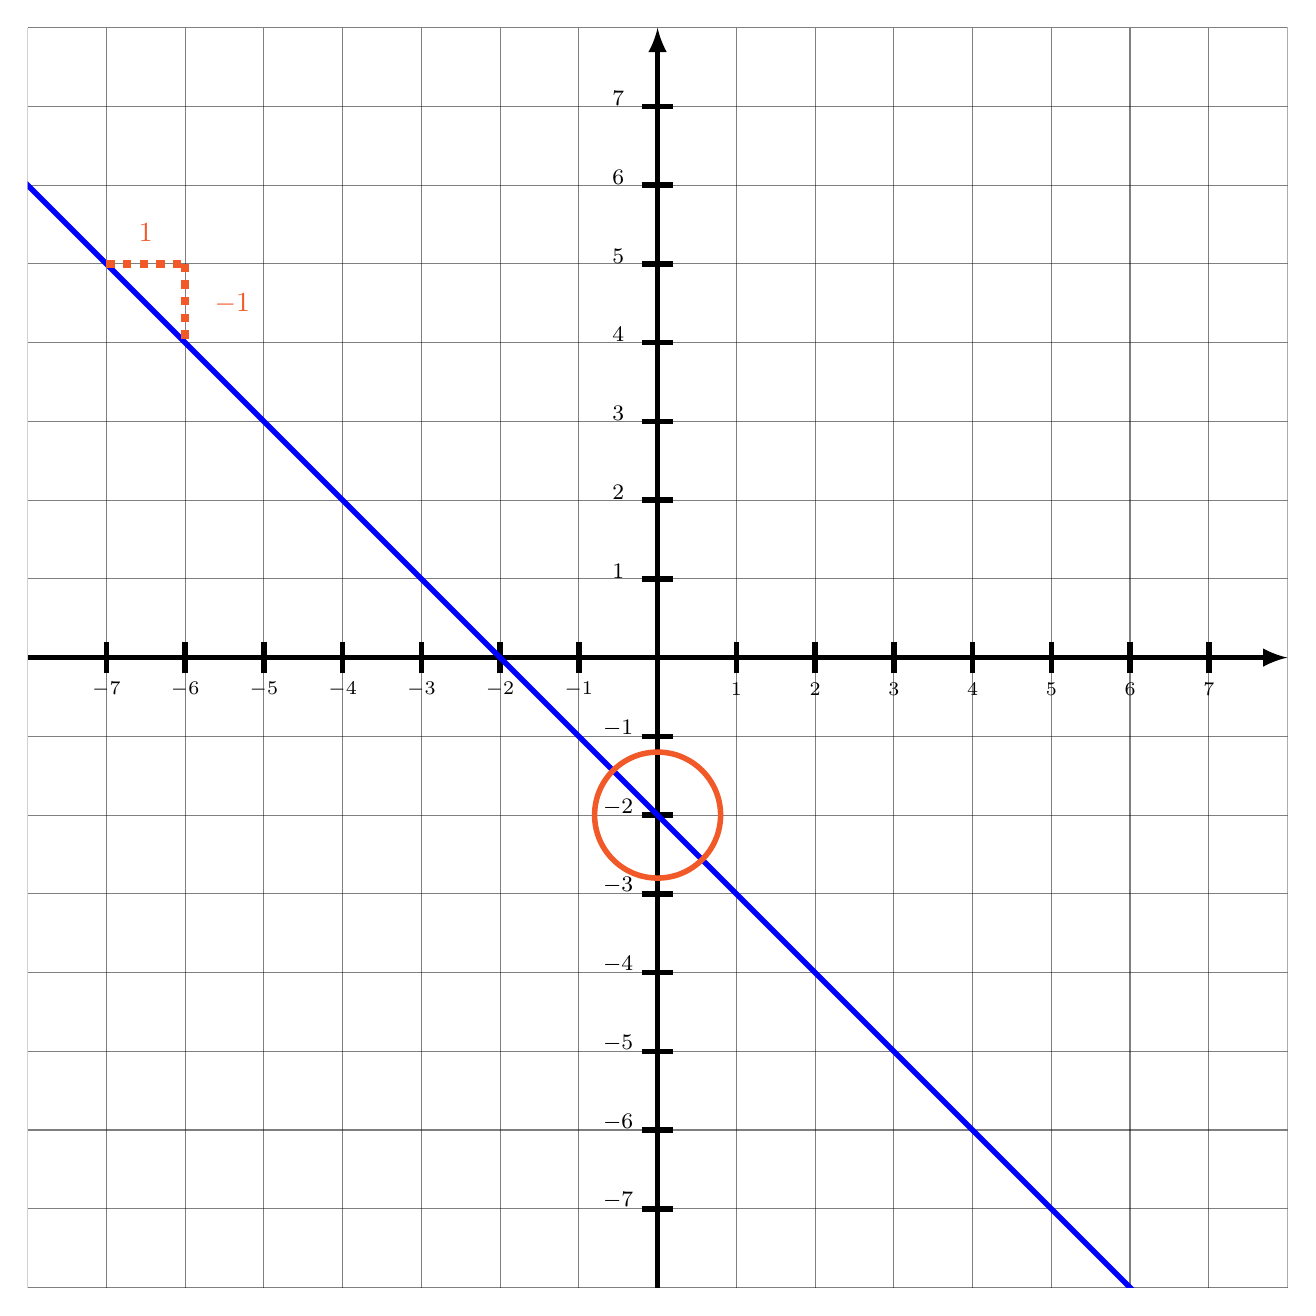
\begin{tikzpicture}[baseline]

    \tikzset{
      point/.style={
        thick,
        draw,
        cross out,
        inner sep=0pt,
        minimum width=5pt,
        minimum height=5pt,
      },
    }
    \clip (-8,-8) rectangle (8,8);
    	
	\draw[color ={black},line width = 2,>=latex,->] (-8,0)--(8,0);
	\draw[color ={black},line width = 2,>=latex,->] (0,-8)--(0,8);
	\draw[color ={black},opacity = 0.5] (-8,1)--(8,1);
	\draw[color ={black},opacity = 0.5] (-8,2)--(8,2);
	\draw[color ={black},opacity = 0.5] (-8,3)--(8,3);
	\draw[color ={black},opacity = 0.5] (-8,4)--(8,4);
	\draw[color ={black},opacity = 0.5] (-8,5)--(8,5);
	\draw[color ={black},opacity = 0.5] (-8,6)--(8,6);
	\draw[color ={black},opacity = 0.5] (-8,7)--(8,7);
	\draw[color ={black},opacity = 0.5] (-8,8)--(8,8);
	\draw[color ={black},opacity = 0.5] (-8,-1)--(8,-1);
	\draw[color ={black},opacity = 0.5] (-8,-2)--(8,-2);
	\draw[color ={black},opacity = 0.5] (-8,-3)--(8,-3);
	\draw[color ={black},opacity = 0.5] (-8,-4)--(8,-4);
	\draw[color ={black},opacity = 0.5] (-8,-5)--(8,-5);
	\draw[color ={black},opacity = 0.5] (-8,-6)--(8,-6);
	\draw[color ={black},opacity = 0.5] (-8,-7)--(8,-7);
	\draw[color ={black},opacity = 0.5] (-8,-8)--(8,-8);
	\draw[color ={black},opacity = 0.5] (1,-8)--(1,8);
	\draw[color ={black},opacity = 0.5] (2,-8)--(2,8);
	\draw[color ={black},opacity = 0.5] (3,-8)--(3,8);
	\draw[color ={black},opacity = 0.5] (4,-8)--(4,8);
	\draw[color ={black},opacity = 0.5] (5,-8)--(5,8);
	\draw[color ={black},opacity = 0.5] (6,-8)--(6,8);
	\draw[color ={black},opacity = 0.5] (7,-8)--(7,8);
	\draw[color ={black},opacity = 0.5] (8,-8)--(8,8);
	\draw[color ={black},opacity = 0.5] (-1,-8)--(-1,8);
	\draw[color ={black},opacity = 0.5] (-2,-8)--(-2,8);
	\draw[color ={black},opacity = 0.5] (-3,-8)--(-3,8);
	\draw[color ={black},opacity = 0.5] (-4,-8)--(-4,8);
	\draw[color ={black},opacity = 0.5] (-5,-8)--(-5,8);
	\draw[color ={black},opacity = 0.5] (-6,-8)--(-6,8);
	\draw[color ={black},opacity = 0.5] (-7,-8)--(-7,8);
	\draw[color ={black},opacity = 0.5] (-8,-8)--(-8,8);
	\draw[color ={black},line width = 2] (1,-0.2)--(1,0.2);
	\draw[color ={black},line width = 2] (2,-0.2)--(2,0.2);
	\draw[color ={black},line width = 2] (3,-0.2)--(3,0.2);
	\draw[color ={black},line width = 2] (4,-0.2)--(4,0.2);
	\draw[color ={black},line width = 2] (5,-0.2)--(5,0.2);
	\draw[color ={black},line width = 2] (6,-0.2)--(6,0.2);
	\draw[color ={black},line width = 2] (7,-0.2)--(7,0.2);
	\draw[color ={black},line width = 2] (-1,-0.2)--(-1,0.2);
	\draw[color ={black},line width = 2] (-2,-0.2)--(-2,0.2);
	\draw[color ={black},line width = 2] (-3,-0.2)--(-3,0.2);
	\draw[color ={black},line width = 2] (-4,-0.2)--(-4,0.2);
	\draw[color ={black},line width = 2] (-5,-0.2)--(-5,0.2);
	\draw[color ={black},line width = 2] (-6,-0.2)--(-6,0.2);
	\draw[color ={black},line width = 2] (-7,-0.2)--(-7,0.2);
	\draw[color ={black},line width = 2] (-0.2,1)--(0.2,1);
	\draw[color ={black},line width = 2] (-0.2,2)--(0.2,2);
	\draw[color ={black},line width = 2] (-0.2,3)--(0.2,3);
	\draw[color ={black},line width = 2] (-0.2,4)--(0.2,4);
	\draw[color ={black},line width = 2] (-0.2,5)--(0.2,5);
	\draw[color ={black},line width = 2] (-0.2,6)--(0.2,6);
	\draw[color ={black},line width = 2] (-0.2,7)--(0.2,7);
	\draw[color ={black},line width = 2] (-0.2,-1)--(0.2,-1);
	\draw[color ={black},line width = 2] (-0.2,-2)--(0.2,-2);
	\draw[color ={black},line width = 2] (-0.2,-3)--(0.2,-3);
	\draw[color ={black},line width = 2] (-0.2,-4)--(0.2,-4);
	\draw[color ={black},line width = 2] (-0.2,-5)--(0.2,-5);
	\draw[color ={black},line width = 2] (-0.2,-6)--(0.2,-6);
	\draw[color ={black},line width = 2] (-0.2,-7)--(0.2,-7);
	\draw (1,-0.4) node[anchor = center] {\scriptsize \color{black}{$1$}};
	\draw (2,-0.4) node[anchor = center] {\scriptsize \color{black}{$2$}};
	\draw (3,-0.4) node[anchor = center] {\scriptsize \color{black}{$3$}};
	\draw (4,-0.4) node[anchor = center] {\scriptsize \color{black}{$4$}};
	\draw (5,-0.4) node[anchor = center] {\scriptsize \color{black}{$5$}};
	\draw (6,-0.4) node[anchor = center] {\scriptsize \color{black}{$6$}};
	\draw (7,-0.4) node[anchor = center] {\scriptsize \color{black}{$7$}};
	\draw (-1,-0.4) node[anchor = center] {\scriptsize \color{black}{$-1$}};
	\draw (-2,-0.4) node[anchor = center] {\scriptsize \color{black}{$-2$}};
	\draw (-3,-0.4) node[anchor = center] {\scriptsize \color{black}{$-3$}};
	\draw (-4,-0.4) node[anchor = center] {\scriptsize \color{black}{$-4$}};
	\draw (-5,-0.4) node[anchor = center] {\scriptsize \color{black}{$-5$}};
	\draw (-6,-0.4) node[anchor = center] {\scriptsize \color{black}{$-6$}};
	\draw (-7,-0.4) node[anchor = center] {\scriptsize \color{black}{$-7$}};
	\draw (-0.5,1.1) node[anchor = center] {\footnotesize \color{black}{$1$}};
	\draw (-0.5,2.1) node[anchor = center] {\footnotesize \color{black}{$2$}};
	\draw (-0.5,3.1) node[anchor = center] {\footnotesize \color{black}{$3$}};
	\draw (-0.5,4.1) node[anchor = center] {\footnotesize \color{black}{$4$}};
	\draw (-0.5,5.1) node[anchor = center] {\footnotesize \color{black}{$5$}};
	\draw (-0.5,6.1) node[anchor = center] {\footnotesize \color{black}{$6$}};
	\draw (-0.5,7.1) node[anchor = center] {\footnotesize \color{black}{$7$}};
	\draw (-0.5,-0.9) node[anchor = center] {\footnotesize \color{black}{$-1$}};
	\draw (-0.5,-1.9) node[anchor = center] {\footnotesize \color{black}{$-2$}};
	\draw (-0.5,-2.9) node[anchor = center] {\footnotesize \color{black}{$-3$}};
	\draw (-0.5,-3.9) node[anchor = center] {\footnotesize \color{black}{$-4$}};
	\draw (-0.5,-4.9) node[anchor = center] {\footnotesize \color{black}{$-5$}};
	\draw (-0.5,-5.9) node[anchor = center] {\footnotesize \color{black}{$-6$}};
	\draw (-0.5,-6.9) node[anchor = center] {\footnotesize \color{black}{$-7$}};
	\draw[color={blue},line width = 2] (-35.355328118658136,33.355328118658136)--(36.355328118658136,-38.355328118658136);
	\draw[color={rgb,255:red,241;green,89;blue,41},line width = 2,fill opacity = 1.1] (0,-2) circle (0.8);
	\draw[color ={rgb,255:red,241;green,89;blue,41},line width = 3, dashed ] (-7,5)--(-6,5);
	\draw[color ={rgb,255:red,241;green,89;blue,41},line width = 3, dashed ] (-6,5)--(-6,4);
	\draw [color={rgb,255:red,241;green,89;blue,41}] (-6.5,5.4) node[anchor = center,scale=1, rotate = 0] {$1$};
	\draw [color={rgb,255:red,241;green,89;blue,41}] (-5.4,4.5) node[anchor = center,scale=1, rotate = 0] {$-1$};

\end{tikzpicture}\\\\\textbf {a.} La droite coupe l'axe des ordonnées au point de coordonnées $(0;-2)$. L'ordonnée de $g$ à l'origine est donc $-2$.\\\textbf {b.} À chaque fois que l'on avance de 1 unité d'abscisses, on descend de $1$ unité d'ordonnées. Le coefficient directeur de $g$ est donc $-1$.\\\textbf {c.} $g$ étant une fonction affine, on a $g : x \mapsto $$ax + b$ avec $a$ son coefficient directeur (ou pente) et $b$ son ordonnée à l'origine.\\Finalement, $g : x \mapsto -x$$-2$.
\item 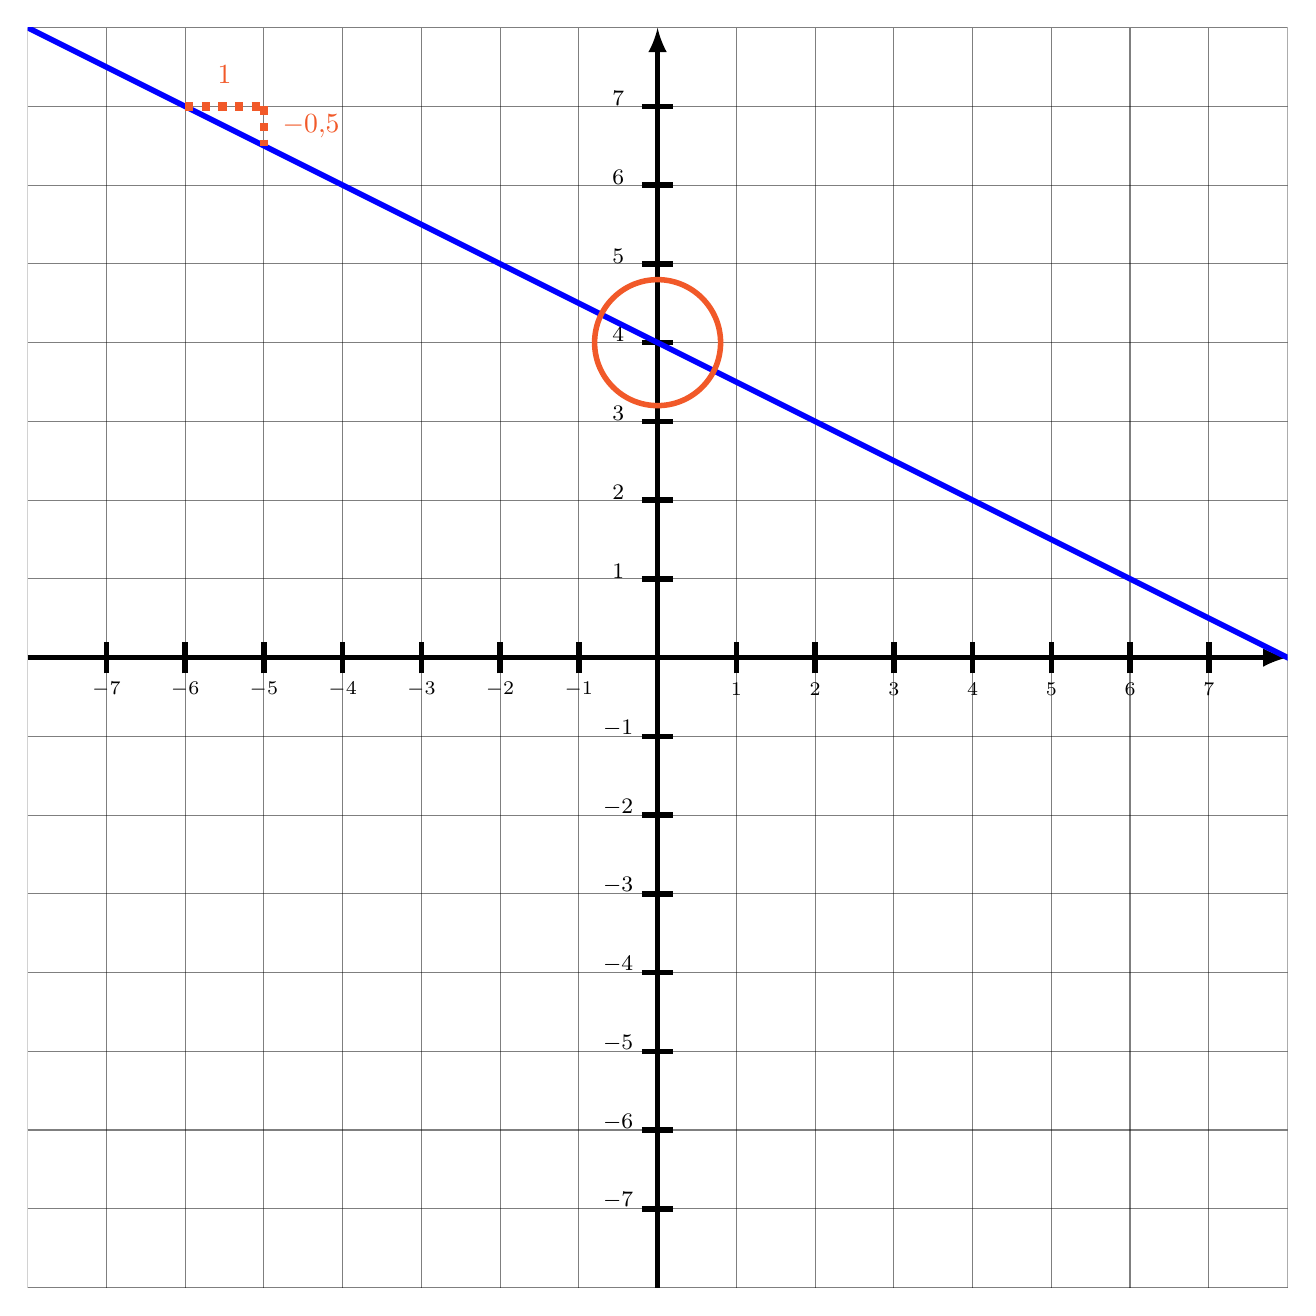
\begin{tikzpicture}[baseline]

    \tikzset{
      point/.style={
        thick,
        draw,
        cross out,
        inner sep=0pt,
        minimum width=5pt,
        minimum height=5pt,
      },
    }
    \clip (-8,-8) rectangle (8,8);
    	
	\draw[color ={black},line width = 2,>=latex,->] (-8,0)--(8,0);
	\draw[color ={black},line width = 2,>=latex,->] (0,-8)--(0,8);
	\draw[color ={black},opacity = 0.5] (-8,1)--(8,1);
	\draw[color ={black},opacity = 0.5] (-8,2)--(8,2);
	\draw[color ={black},opacity = 0.5] (-8,3)--(8,3);
	\draw[color ={black},opacity = 0.5] (-8,4)--(8,4);
	\draw[color ={black},opacity = 0.5] (-8,5)--(8,5);
	\draw[color ={black},opacity = 0.5] (-8,6)--(8,6);
	\draw[color ={black},opacity = 0.5] (-8,7)--(8,7);
	\draw[color ={black},opacity = 0.5] (-8,8)--(8,8);
	\draw[color ={black},opacity = 0.5] (-8,-1)--(8,-1);
	\draw[color ={black},opacity = 0.5] (-8,-2)--(8,-2);
	\draw[color ={black},opacity = 0.5] (-8,-3)--(8,-3);
	\draw[color ={black},opacity = 0.5] (-8,-4)--(8,-4);
	\draw[color ={black},opacity = 0.5] (-8,-5)--(8,-5);
	\draw[color ={black},opacity = 0.5] (-8,-6)--(8,-6);
	\draw[color ={black},opacity = 0.5] (-8,-7)--(8,-7);
	\draw[color ={black},opacity = 0.5] (-8,-8)--(8,-8);
	\draw[color ={black},opacity = 0.5] (1,-8)--(1,8);
	\draw[color ={black},opacity = 0.5] (2,-8)--(2,8);
	\draw[color ={black},opacity = 0.5] (3,-8)--(3,8);
	\draw[color ={black},opacity = 0.5] (4,-8)--(4,8);
	\draw[color ={black},opacity = 0.5] (5,-8)--(5,8);
	\draw[color ={black},opacity = 0.5] (6,-8)--(6,8);
	\draw[color ={black},opacity = 0.5] (7,-8)--(7,8);
	\draw[color ={black},opacity = 0.5] (8,-8)--(8,8);
	\draw[color ={black},opacity = 0.5] (-1,-8)--(-1,8);
	\draw[color ={black},opacity = 0.5] (-2,-8)--(-2,8);
	\draw[color ={black},opacity = 0.5] (-3,-8)--(-3,8);
	\draw[color ={black},opacity = 0.5] (-4,-8)--(-4,8);
	\draw[color ={black},opacity = 0.5] (-5,-8)--(-5,8);
	\draw[color ={black},opacity = 0.5] (-6,-8)--(-6,8);
	\draw[color ={black},opacity = 0.5] (-7,-8)--(-7,8);
	\draw[color ={black},opacity = 0.5] (-8,-8)--(-8,8);
	\draw[color ={black},line width = 2] (1,-0.2)--(1,0.2);
	\draw[color ={black},line width = 2] (2,-0.2)--(2,0.2);
	\draw[color ={black},line width = 2] (3,-0.2)--(3,0.2);
	\draw[color ={black},line width = 2] (4,-0.2)--(4,0.2);
	\draw[color ={black},line width = 2] (5,-0.2)--(5,0.2);
	\draw[color ={black},line width = 2] (6,-0.2)--(6,0.2);
	\draw[color ={black},line width = 2] (7,-0.2)--(7,0.2);
	\draw[color ={black},line width = 2] (-1,-0.2)--(-1,0.2);
	\draw[color ={black},line width = 2] (-2,-0.2)--(-2,0.2);
	\draw[color ={black},line width = 2] (-3,-0.2)--(-3,0.2);
	\draw[color ={black},line width = 2] (-4,-0.2)--(-4,0.2);
	\draw[color ={black},line width = 2] (-5,-0.2)--(-5,0.2);
	\draw[color ={black},line width = 2] (-6,-0.2)--(-6,0.2);
	\draw[color ={black},line width = 2] (-7,-0.2)--(-7,0.2);
	\draw[color ={black},line width = 2] (-0.2,1)--(0.2,1);
	\draw[color ={black},line width = 2] (-0.2,2)--(0.2,2);
	\draw[color ={black},line width = 2] (-0.2,3)--(0.2,3);
	\draw[color ={black},line width = 2] (-0.2,4)--(0.2,4);
	\draw[color ={black},line width = 2] (-0.2,5)--(0.2,5);
	\draw[color ={black},line width = 2] (-0.2,6)--(0.2,6);
	\draw[color ={black},line width = 2] (-0.2,7)--(0.2,7);
	\draw[color ={black},line width = 2] (-0.2,-1)--(0.2,-1);
	\draw[color ={black},line width = 2] (-0.2,-2)--(0.2,-2);
	\draw[color ={black},line width = 2] (-0.2,-3)--(0.2,-3);
	\draw[color ={black},line width = 2] (-0.2,-4)--(0.2,-4);
	\draw[color ={black},line width = 2] (-0.2,-5)--(0.2,-5);
	\draw[color ={black},line width = 2] (-0.2,-6)--(0.2,-6);
	\draw[color ={black},line width = 2] (-0.2,-7)--(0.2,-7);
	\draw (1,-0.4) node[anchor = center] {\scriptsize \color{black}{$1$}};
	\draw (2,-0.4) node[anchor = center] {\scriptsize \color{black}{$2$}};
	\draw (3,-0.4) node[anchor = center] {\scriptsize \color{black}{$3$}};
	\draw (4,-0.4) node[anchor = center] {\scriptsize \color{black}{$4$}};
	\draw (5,-0.4) node[anchor = center] {\scriptsize \color{black}{$5$}};
	\draw (6,-0.4) node[anchor = center] {\scriptsize \color{black}{$6$}};
	\draw (7,-0.4) node[anchor = center] {\scriptsize \color{black}{$7$}};
	\draw (-1,-0.4) node[anchor = center] {\scriptsize \color{black}{$-1$}};
	\draw (-2,-0.4) node[anchor = center] {\scriptsize \color{black}{$-2$}};
	\draw (-3,-0.4) node[anchor = center] {\scriptsize \color{black}{$-3$}};
	\draw (-4,-0.4) node[anchor = center] {\scriptsize \color{black}{$-4$}};
	\draw (-5,-0.4) node[anchor = center] {\scriptsize \color{black}{$-5$}};
	\draw (-6,-0.4) node[anchor = center] {\scriptsize \color{black}{$-6$}};
	\draw (-7,-0.4) node[anchor = center] {\scriptsize \color{black}{$-7$}};
	\draw (-0.5,1.1) node[anchor = center] {\footnotesize \color{black}{$1$}};
	\draw (-0.5,2.1) node[anchor = center] {\footnotesize \color{black}{$2$}};
	\draw (-0.5,3.1) node[anchor = center] {\footnotesize \color{black}{$3$}};
	\draw (-0.5,4.1) node[anchor = center] {\footnotesize \color{black}{$4$}};
	\draw (-0.5,5.1) node[anchor = center] {\footnotesize \color{black}{$5$}};
	\draw (-0.5,6.1) node[anchor = center] {\footnotesize \color{black}{$6$}};
	\draw (-0.5,7.1) node[anchor = center] {\footnotesize \color{black}{$7$}};
	\draw (-0.5,-0.9) node[anchor = center] {\footnotesize \color{black}{$-1$}};
	\draw (-0.5,-1.9) node[anchor = center] {\footnotesize \color{black}{$-2$}};
	\draw (-0.5,-2.9) node[anchor = center] {\footnotesize \color{black}{$-3$}};
	\draw (-0.5,-3.9) node[anchor = center] {\footnotesize \color{black}{$-4$}};
	\draw (-0.5,-4.9) node[anchor = center] {\footnotesize \color{black}{$-5$}};
	\draw (-0.5,-5.9) node[anchor = center] {\footnotesize \color{black}{$-6$}};
	\draw (-0.5,-6.9) node[anchor = center] {\footnotesize \color{black}{$-7$}};
	\draw[color={blue},line width = 2] (-44.721359099991595,26.360679549995798)--(45.721359099991595,-18.860679549995798);
	\draw[color={rgb,255:red,241;green,89;blue,41},line width = 2,fill opacity = 1.1] (0,4) circle (0.8);
	\draw[color ={rgb,255:red,241;green,89;blue,41},line width = 3, dashed ] (-6,7)--(-5,7);
	\draw[color ={rgb,255:red,241;green,89;blue,41},line width = 3, dashed ] (-5,7)--(-5,6.5);
	\draw [color={rgb,255:red,241;green,89;blue,41}] (-5.5,7.4) node[anchor = center,scale=1, rotate = 0] {$1$};
	\draw [color={rgb,255:red,241;green,89;blue,41}] (-4.4,6.75) node[anchor = center,scale=1, rotate = 0] {$-0{,}5$};

\end{tikzpicture}\\\\\textbf {a.} La droite coupe l'axe des ordonnées au point de coordonnées $(0;4)$. L'ordonnée de $f_3$ à l'origine est donc $4$.\\\textbf {b.} À chaque fois que l'on avance de 1 unité d'abscisses, on descend de $0{,}5$ unité d'ordonnées. Le coefficient directeur de $f_3$ est donc $-0{,}5$.\\\textbf {c.} $f_3$ étant une fonction affine, on a $f_3 : x \mapsto $$ax + b$ avec $a$ son coefficient directeur (ou pente) et $b$ son ordonnée à l'origine.\\Finalement, $f_3 : x \mapsto -0,5x$$+4$.
\end{enumerate}

\end{EXO}

\begin{EXO}{}{}

\begin{enumerate}[]
\item $f$ est une fonction affine, elle a donc une expression de la forme  $f(x)=ax+b$ avec $a$ et $b$ des nombres réels.
                        \\D'après le cours, on sait que pour $u\neq v$, $a=\dfrac{f(u)-f(v)}{u-v}$ \\Avec $u=4$ et  $v=7$, on obtient  :  $a=\dfrac{f(4)-f(7)}{4-7}=\dfrac{27-42}{4-7}=\dfrac{-15}{-3}=5$.\\On en déduit que la fonction $f$ s'écrit sous la forme :    $f(x)=5 x +b.$\\\textbf{Remarque : }On obtient $b$ en utilisant (au choix) une des deux données de l'énoncé, par exemple $f(4)=27$.\\Comme $f(x)=5x +b$, alors $f(4)=
              5\cdot4+b=20+b$ . On en déduit :\\$\begin{aligned}f(4)=27&\iff 20+b=27\\&\iff b=7\\\end{aligned}$\\On en déduit $f(x)=5x+7$.
\item $f$ est une fonction affine, elle a donc une expression de la forme  $f(x)=ax+b$ avec $a$ et $b$ des nombres réels.
                        \\D'après le cours, on sait que pour $u\neq v$, $a=\dfrac{f(u)-f(v)}{u-v}$ \\Avec $u=3$ et  $v=9$, on obtient  :  $a=\dfrac{f(3)-f(9)}{3-9}=\dfrac{-15-(-33)}{3-9}=\dfrac{18}{-6}=-3$.\\On en déduit que la fonction $f$ s'écrit sous la forme :    $f(x)=-3 x +b.$\\\textbf{Remarque : }On obtient $b$ en utilisant (au choix) une des deux données de l'énoncé, par exemple $f(3)=-15$.\\Comme $f(x)=-3x +b$, alors $f(3)=
              -3\cdot3+b=-9+b$ . On en déduit :\\$\begin{aligned}f(3)=-15&\iff -9+b=-15\\&\iff b=-6\\\end{aligned}$\\On en déduit $f(x)=-3x-6$.
\item $f$ est une fonction affine, elle a donc une expression de la forme  $f(x)=ax+b$ avec $a$ et $b$ des nombres réels.
                        \\D'après le cours, on sait que pour $u\neq v$, $a=\dfrac{f(u)-f(v)}{u-v}$ \\Avec $u=6$ et  $v=9$, on obtient  :  $a=\dfrac{f(6)-f(9)}{6-9}=\dfrac{16-25}{6-9}=\dfrac{-9}{-3}=3$.\\On en déduit que la fonction $f$ s'écrit sous la forme :    $f(x)=3 x +b.$\\\textbf{Remarque : }On obtient $b$ en utilisant (au choix) une des deux données de l'énoncé, par exemple $f(6)=16$.\\Comme $f(x)=3x +b$, alors $f(6)=
              3\cdot6+b=18+b$ . On en déduit :\\$\begin{aligned}f(6)=16&\iff 18+b=16\\&\iff b=-2\\\end{aligned}$\\On en déduit $f(x)=3x-2$.
\end{enumerate}

\end{EXO}

\begin{EXO}{}{}

 La droite $d_1$ passe par le point de coordonnées $(0;-4)$. Elle représente donc la fonction affine $f_1(x)=ax+b$ dont la constante $b$ est égale à $f_1(0)=a\cdot 0+b$, c'est-à-dire  $-4=0+b$ donc $b=-4$.\\ De plus $(d_1)$ passe par le point de coordonnées $(1;-7)$ donc $f_1(1)=-7=a\cdot 1-4=a-4$ donc $a=-7+4=-3$. Ainsi $f_1(x)={\color[HTML]{f15929}\boldsymbol{-3x-4}}$.
 La droite $d_2$ passe par le point de coordonnées $(0;1)$. Elle représente donc la fonction affine $f_2(x)=ax+b$ dont la constante $b$ est égale à $f_2(0)=a\cdot 0+b$, c'est-à-dire  $1=0+b$ donc $b=1$.\\ De plus $(d_2)$ passe par le point de coordonnées $(1;3)$ donc $f_2(1)=3=a\cdot 1+1=a+1$ donc $a=3-1=2$. Ainsi $f_2(x)={\color[HTML]{f15929}\boldsymbol{2x+1}}$.
 La droite $d_3$ passe par le point de coordonnées $(0;-2)$. Elle représente donc la fonction affine $f_3(x)=ax+b$ dont la constante $b$ est égale à $f_3(0)=a\cdot 0+b$, c'est-à-dire  $-2=0+b$ donc $b=-2$.\\ De plus $(d_3)$ passe par le point de coordonnées $(1;-3)$ donc $f_3(1)=-3=a\cdot 1-2=a-2$ donc $a=-3+2=-1$. Ainsi $f_3(x)={\color[HTML]{f15929}\boldsymbol{-x-2}}$.
\end{EXO}

\clearpage
\end{Correction}
\end{document}

% Local Variables:
% TeX-engine: luatex
% End:
% Local Variables:
% TeX-engine: luatex
% End:
